\documentclass{article}

\usepackage{amsmath}

\usepackage{mathrsfs}

\usepackage{graphicx}

\usepackage{hyperref}

\usepackage[utf8]{inputenc}

\usepackage{subcaption}

\usepackage{geometry}

\usepackage{multirow}

\usepackage{siunitx}

\usepackage[square,numbers]{natbib}

\usepackage[english]{babel}
%Includes "References" in the table of contents
\usepackage[nottoc]{tocbibind}

\usepackage[parfill]{parskip}

\usepackage[toc,page]{appendix}

\usepackage{tabularx}

\usepackage{booktabs}

\usepackage{pgfplots}

\usepackage{adjustbox}

\usepackage{lmodern}

\usepackage{subcaption}

\makeatletter\@ifpackageloaded{underscore}{}{\usepackage[strings]{underscore}}\makeatother

\newcommand{\pvec}[1]{\vec{#1}\mkern2mu\vphantom{#1}}

\pgfplotsset{width=10cm,compat=1.9}

\DeclareSIUnit{\angstrom}{\textup{\AA}}

\geometry{legalpaper, portrait, margin=1in}

\title{Lab Report}

\author{Jamal Ghaith}
\author{Anas Roumieh}

\date{01.04.2024}

\begin{document}


\begin{titlepage}
	\centering
	{\scshape\LARGE University of Leipzig \par}
	\vspace{1cm}
	{\scshape\ Advanced Labs\par}
	\vspace{1.5cm}
	{\huge\bfseries Lab report\par}
	\vspace{2cm}
	{\huge\bfseries Doppler-free Rb saturation spectroscopy with an external cavity diode laser\par}
	\vspace{2cm}
	{\Large Jamal Ghaith 3792970\par}
    {\Large Anas Roumieh 3766647\par}
	\vfill

    {\Large Conducted on:  14.05.2024\par}
	\vfill
\end{titlepage}

\tableofcontents
\pagenumbering{gobble}
\pagebreak{}
\pagenumbering{arabic}

\section{Introduction}

\begin{equation}
	\mathscr{F} = \frac{\nu_{\text{FSR}}}{\delta \nu}
	\label{eq:finesse}
\end{equation}

\pagebreak{}

\section{Analysis}

\subsection{Task 1}

We were instructed to scale our measurement data using the FPI peaks in addition to determining the finesse.

\subsubsection{Scaling the data}

From \cite{jung_2018_dopplerfree}, we know that our FSR is $1$ GHz. Therefore, if the average spacing between peaks is calculated, we can determine the conversion factor and scale our data accordingly.

\begin{figure}[h]
	\centering
	\begin{subfigure}[t]{0.45\textwidth}
		\centering
		\scalebox{0.5}{%% Creator: Matplotlib, PGF backend
%%
%% To include the figure in your LaTeX document, write
%%   \input{<filename>.pgf}
%%
%% Make sure the required packages are loaded in your preamble
%%   \usepackage{pgf}
%%
%% Also ensure that all the required font packages are loaded; for instance,
%% the lmodern package is sometimes necessary when using math font.
%%   \usepackage{lmodern}
%%
%% Figures using additional raster images can only be included by \input if
%% they are in the same directory as the main LaTeX file. For loading figures
%% from other directories you can use the `import` package
%%   \usepackage{import}
%%
%% and then include the figures with
%%   \import{<path to file>}{<filename>.pgf}
%%
%% Matplotlib used the following preamble
%%   
%%   \usepackage{fontspec}
%%   \makeatletter\@ifpackageloaded{underscore}{}{\usepackage[strings]{underscore}}\makeatother
%%
\begingroup%
\makeatletter%
\begin{pgfpicture}%
\pgfpathrectangle{\pgfpointorigin}{\pgfqpoint{6.489553in}{4.010764in}}%
\pgfusepath{use as bounding box, clip}%
\begin{pgfscope}%
\pgfsetbuttcap%
\pgfsetmiterjoin%
\definecolor{currentfill}{rgb}{1.000000,1.000000,1.000000}%
\pgfsetfillcolor{currentfill}%
\pgfsetlinewidth{0.000000pt}%
\definecolor{currentstroke}{rgb}{1.000000,1.000000,1.000000}%
\pgfsetstrokecolor{currentstroke}%
\pgfsetdash{}{0pt}%
\pgfpathmoveto{\pgfqpoint{0.000000in}{0.000000in}}%
\pgfpathlineto{\pgfqpoint{6.489553in}{0.000000in}}%
\pgfpathlineto{\pgfqpoint{6.489553in}{4.010764in}}%
\pgfpathlineto{\pgfqpoint{0.000000in}{4.010764in}}%
\pgfpathlineto{\pgfqpoint{0.000000in}{0.000000in}}%
\pgfpathclose%
\pgfusepath{fill}%
\end{pgfscope}%
\begin{pgfscope}%
\pgfsetbuttcap%
\pgfsetmiterjoin%
\definecolor{currentfill}{rgb}{1.000000,1.000000,1.000000}%
\pgfsetfillcolor{currentfill}%
\pgfsetlinewidth{0.000000pt}%
\definecolor{currentstroke}{rgb}{0.000000,0.000000,0.000000}%
\pgfsetstrokecolor{currentstroke}%
\pgfsetstrokeopacity{0.000000}%
\pgfsetdash{}{0pt}%
\pgfpathmoveto{\pgfqpoint{0.811194in}{0.441184in}}%
\pgfpathlineto{\pgfqpoint{5.840598in}{0.441184in}}%
\pgfpathlineto{\pgfqpoint{5.840598in}{3.529473in}}%
\pgfpathlineto{\pgfqpoint{0.811194in}{3.529473in}}%
\pgfpathlineto{\pgfqpoint{0.811194in}{0.441184in}}%
\pgfpathclose%
\pgfusepath{fill}%
\end{pgfscope}%
\begin{pgfscope}%
\pgfsetbuttcap%
\pgfsetroundjoin%
\definecolor{currentfill}{rgb}{0.000000,0.000000,0.000000}%
\pgfsetfillcolor{currentfill}%
\pgfsetlinewidth{0.803000pt}%
\definecolor{currentstroke}{rgb}{0.000000,0.000000,0.000000}%
\pgfsetstrokecolor{currentstroke}%
\pgfsetdash{}{0pt}%
\pgfsys@defobject{currentmarker}{\pgfqpoint{0.000000in}{-0.048611in}}{\pgfqpoint{0.000000in}{0.000000in}}{%
\pgfpathmoveto{\pgfqpoint{0.000000in}{0.000000in}}%
\pgfpathlineto{\pgfqpoint{0.000000in}{-0.048611in}}%
\pgfusepath{stroke,fill}%
}%
\begin{pgfscope}%
\pgfsys@transformshift{0.893643in}{0.441184in}%
\pgfsys@useobject{currentmarker}{}%
\end{pgfscope}%
\end{pgfscope}%
\begin{pgfscope}%
\definecolor{textcolor}{rgb}{0.000000,0.000000,0.000000}%
\pgfsetstrokecolor{textcolor}%
\pgfsetfillcolor{textcolor}%
\pgftext[x=0.893643in,y=0.343962in,,top]{\color{textcolor}\rmfamily\fontsize{10.000000}{12.000000}\selectfont \(\displaystyle {0}\)}%
\end{pgfscope}%
\begin{pgfscope}%
\pgfsetbuttcap%
\pgfsetroundjoin%
\definecolor{currentfill}{rgb}{0.000000,0.000000,0.000000}%
\pgfsetfillcolor{currentfill}%
\pgfsetlinewidth{0.803000pt}%
\definecolor{currentstroke}{rgb}{0.000000,0.000000,0.000000}%
\pgfsetstrokecolor{currentstroke}%
\pgfsetdash{}{0pt}%
\pgfsys@defobject{currentmarker}{\pgfqpoint{0.000000in}{-0.048611in}}{\pgfqpoint{0.000000in}{0.000000in}}{%
\pgfpathmoveto{\pgfqpoint{0.000000in}{0.000000in}}%
\pgfpathlineto{\pgfqpoint{0.000000in}{-0.048611in}}%
\pgfusepath{stroke,fill}%
}%
\begin{pgfscope}%
\pgfsys@transformshift{1.718136in}{0.441184in}%
\pgfsys@useobject{currentmarker}{}%
\end{pgfscope}%
\end{pgfscope}%
\begin{pgfscope}%
\definecolor{textcolor}{rgb}{0.000000,0.000000,0.000000}%
\pgfsetstrokecolor{textcolor}%
\pgfsetfillcolor{textcolor}%
\pgftext[x=1.718136in,y=0.343962in,,top]{\color{textcolor}\rmfamily\fontsize{10.000000}{12.000000}\selectfont \(\displaystyle {100}\)}%
\end{pgfscope}%
\begin{pgfscope}%
\pgfsetbuttcap%
\pgfsetroundjoin%
\definecolor{currentfill}{rgb}{0.000000,0.000000,0.000000}%
\pgfsetfillcolor{currentfill}%
\pgfsetlinewidth{0.803000pt}%
\definecolor{currentstroke}{rgb}{0.000000,0.000000,0.000000}%
\pgfsetstrokecolor{currentstroke}%
\pgfsetdash{}{0pt}%
\pgfsys@defobject{currentmarker}{\pgfqpoint{0.000000in}{-0.048611in}}{\pgfqpoint{0.000000in}{0.000000in}}{%
\pgfpathmoveto{\pgfqpoint{0.000000in}{0.000000in}}%
\pgfpathlineto{\pgfqpoint{0.000000in}{-0.048611in}}%
\pgfusepath{stroke,fill}%
}%
\begin{pgfscope}%
\pgfsys@transformshift{2.542628in}{0.441184in}%
\pgfsys@useobject{currentmarker}{}%
\end{pgfscope}%
\end{pgfscope}%
\begin{pgfscope}%
\definecolor{textcolor}{rgb}{0.000000,0.000000,0.000000}%
\pgfsetstrokecolor{textcolor}%
\pgfsetfillcolor{textcolor}%
\pgftext[x=2.542628in,y=0.343962in,,top]{\color{textcolor}\rmfamily\fontsize{10.000000}{12.000000}\selectfont \(\displaystyle {200}\)}%
\end{pgfscope}%
\begin{pgfscope}%
\pgfsetbuttcap%
\pgfsetroundjoin%
\definecolor{currentfill}{rgb}{0.000000,0.000000,0.000000}%
\pgfsetfillcolor{currentfill}%
\pgfsetlinewidth{0.803000pt}%
\definecolor{currentstroke}{rgb}{0.000000,0.000000,0.000000}%
\pgfsetstrokecolor{currentstroke}%
\pgfsetdash{}{0pt}%
\pgfsys@defobject{currentmarker}{\pgfqpoint{0.000000in}{-0.048611in}}{\pgfqpoint{0.000000in}{0.000000in}}{%
\pgfpathmoveto{\pgfqpoint{0.000000in}{0.000000in}}%
\pgfpathlineto{\pgfqpoint{0.000000in}{-0.048611in}}%
\pgfusepath{stroke,fill}%
}%
\begin{pgfscope}%
\pgfsys@transformshift{3.367121in}{0.441184in}%
\pgfsys@useobject{currentmarker}{}%
\end{pgfscope}%
\end{pgfscope}%
\begin{pgfscope}%
\definecolor{textcolor}{rgb}{0.000000,0.000000,0.000000}%
\pgfsetstrokecolor{textcolor}%
\pgfsetfillcolor{textcolor}%
\pgftext[x=3.367121in,y=0.343962in,,top]{\color{textcolor}\rmfamily\fontsize{10.000000}{12.000000}\selectfont \(\displaystyle {300}\)}%
\end{pgfscope}%
\begin{pgfscope}%
\pgfsetbuttcap%
\pgfsetroundjoin%
\definecolor{currentfill}{rgb}{0.000000,0.000000,0.000000}%
\pgfsetfillcolor{currentfill}%
\pgfsetlinewidth{0.803000pt}%
\definecolor{currentstroke}{rgb}{0.000000,0.000000,0.000000}%
\pgfsetstrokecolor{currentstroke}%
\pgfsetdash{}{0pt}%
\pgfsys@defobject{currentmarker}{\pgfqpoint{0.000000in}{-0.048611in}}{\pgfqpoint{0.000000in}{0.000000in}}{%
\pgfpathmoveto{\pgfqpoint{0.000000in}{0.000000in}}%
\pgfpathlineto{\pgfqpoint{0.000000in}{-0.048611in}}%
\pgfusepath{stroke,fill}%
}%
\begin{pgfscope}%
\pgfsys@transformshift{4.191613in}{0.441184in}%
\pgfsys@useobject{currentmarker}{}%
\end{pgfscope}%
\end{pgfscope}%
\begin{pgfscope}%
\definecolor{textcolor}{rgb}{0.000000,0.000000,0.000000}%
\pgfsetstrokecolor{textcolor}%
\pgfsetfillcolor{textcolor}%
\pgftext[x=4.191613in,y=0.343962in,,top]{\color{textcolor}\rmfamily\fontsize{10.000000}{12.000000}\selectfont \(\displaystyle {400}\)}%
\end{pgfscope}%
\begin{pgfscope}%
\pgfsetbuttcap%
\pgfsetroundjoin%
\definecolor{currentfill}{rgb}{0.000000,0.000000,0.000000}%
\pgfsetfillcolor{currentfill}%
\pgfsetlinewidth{0.803000pt}%
\definecolor{currentstroke}{rgb}{0.000000,0.000000,0.000000}%
\pgfsetstrokecolor{currentstroke}%
\pgfsetdash{}{0pt}%
\pgfsys@defobject{currentmarker}{\pgfqpoint{0.000000in}{-0.048611in}}{\pgfqpoint{0.000000in}{0.000000in}}{%
\pgfpathmoveto{\pgfqpoint{0.000000in}{0.000000in}}%
\pgfpathlineto{\pgfqpoint{0.000000in}{-0.048611in}}%
\pgfusepath{stroke,fill}%
}%
\begin{pgfscope}%
\pgfsys@transformshift{5.016105in}{0.441184in}%
\pgfsys@useobject{currentmarker}{}%
\end{pgfscope}%
\end{pgfscope}%
\begin{pgfscope}%
\definecolor{textcolor}{rgb}{0.000000,0.000000,0.000000}%
\pgfsetstrokecolor{textcolor}%
\pgfsetfillcolor{textcolor}%
\pgftext[x=5.016105in,y=0.343962in,,top]{\color{textcolor}\rmfamily\fontsize{10.000000}{12.000000}\selectfont \(\displaystyle {500}\)}%
\end{pgfscope}%
\begin{pgfscope}%
\pgfsetbuttcap%
\pgfsetroundjoin%
\definecolor{currentfill}{rgb}{0.000000,0.000000,0.000000}%
\pgfsetfillcolor{currentfill}%
\pgfsetlinewidth{0.803000pt}%
\definecolor{currentstroke}{rgb}{0.000000,0.000000,0.000000}%
\pgfsetstrokecolor{currentstroke}%
\pgfsetdash{}{0pt}%
\pgfsys@defobject{currentmarker}{\pgfqpoint{0.000000in}{-0.048611in}}{\pgfqpoint{0.000000in}{0.000000in}}{%
\pgfpathmoveto{\pgfqpoint{0.000000in}{0.000000in}}%
\pgfpathlineto{\pgfqpoint{0.000000in}{-0.048611in}}%
\pgfusepath{stroke,fill}%
}%
\begin{pgfscope}%
\pgfsys@transformshift{5.840598in}{0.441184in}%
\pgfsys@useobject{currentmarker}{}%
\end{pgfscope}%
\end{pgfscope}%
\begin{pgfscope}%
\definecolor{textcolor}{rgb}{0.000000,0.000000,0.000000}%
\pgfsetstrokecolor{textcolor}%
\pgfsetfillcolor{textcolor}%
\pgftext[x=5.840598in,y=0.343962in,,top]{\color{textcolor}\rmfamily\fontsize{10.000000}{12.000000}\selectfont \(\displaystyle {600}\)}%
\end{pgfscope}%
\begin{pgfscope}%
\definecolor{textcolor}{rgb}{0.000000,0.000000,0.000000}%
\pgfsetstrokecolor{textcolor}%
\pgfsetfillcolor{textcolor}%
\pgftext[x=3.325896in,y=0.165073in,,top]{\color{textcolor}\rmfamily\fontsize{10.000000}{12.000000}\selectfont Counts [a.u.]}%
\end{pgfscope}%
\begin{pgfscope}%
\pgfsetbuttcap%
\pgfsetroundjoin%
\definecolor{currentfill}{rgb}{0.000000,0.000000,0.000000}%
\pgfsetfillcolor{currentfill}%
\pgfsetlinewidth{0.803000pt}%
\definecolor{currentstroke}{rgb}{0.000000,0.000000,0.000000}%
\pgfsetstrokecolor{currentstroke}%
\pgfsetdash{}{0pt}%
\pgfsys@defobject{currentmarker}{\pgfqpoint{-0.048611in}{0.000000in}}{\pgfqpoint{-0.000000in}{0.000000in}}{%
\pgfpathmoveto{\pgfqpoint{-0.000000in}{0.000000in}}%
\pgfpathlineto{\pgfqpoint{-0.048611in}{0.000000in}}%
\pgfusepath{stroke,fill}%
}%
\begin{pgfscope}%
\pgfsys@transformshift{0.811194in}{0.493274in}%
\pgfsys@useobject{currentmarker}{}%
\end{pgfscope}%
\end{pgfscope}%
\begin{pgfscope}%
\definecolor{textcolor}{rgb}{0.000000,0.000000,0.000000}%
\pgfsetstrokecolor{textcolor}%
\pgfsetfillcolor{textcolor}%
\pgftext[x=0.428477in, y=0.445079in, left, base]{\color{textcolor}\rmfamily\fontsize{10.000000}{12.000000}\selectfont \(\displaystyle {\ensuremath{-}1.6}\)}%
\end{pgfscope}%
\begin{pgfscope}%
\pgfsetbuttcap%
\pgfsetroundjoin%
\definecolor{currentfill}{rgb}{0.000000,0.000000,0.000000}%
\pgfsetfillcolor{currentfill}%
\pgfsetlinewidth{0.803000pt}%
\definecolor{currentstroke}{rgb}{0.000000,0.000000,0.000000}%
\pgfsetstrokecolor{currentstroke}%
\pgfsetdash{}{0pt}%
\pgfsys@defobject{currentmarker}{\pgfqpoint{-0.048611in}{0.000000in}}{\pgfqpoint{-0.000000in}{0.000000in}}{%
\pgfpathmoveto{\pgfqpoint{-0.000000in}{0.000000in}}%
\pgfpathlineto{\pgfqpoint{-0.048611in}{0.000000in}}%
\pgfusepath{stroke,fill}%
}%
\begin{pgfscope}%
\pgfsys@transformshift{0.811194in}{0.846423in}%
\pgfsys@useobject{currentmarker}{}%
\end{pgfscope}%
\end{pgfscope}%
\begin{pgfscope}%
\definecolor{textcolor}{rgb}{0.000000,0.000000,0.000000}%
\pgfsetstrokecolor{textcolor}%
\pgfsetfillcolor{textcolor}%
\pgftext[x=0.428477in, y=0.798228in, left, base]{\color{textcolor}\rmfamily\fontsize{10.000000}{12.000000}\selectfont \(\displaystyle {\ensuremath{-}1.4}\)}%
\end{pgfscope}%
\begin{pgfscope}%
\pgfsetbuttcap%
\pgfsetroundjoin%
\definecolor{currentfill}{rgb}{0.000000,0.000000,0.000000}%
\pgfsetfillcolor{currentfill}%
\pgfsetlinewidth{0.803000pt}%
\definecolor{currentstroke}{rgb}{0.000000,0.000000,0.000000}%
\pgfsetstrokecolor{currentstroke}%
\pgfsetdash{}{0pt}%
\pgfsys@defobject{currentmarker}{\pgfqpoint{-0.048611in}{0.000000in}}{\pgfqpoint{-0.000000in}{0.000000in}}{%
\pgfpathmoveto{\pgfqpoint{-0.000000in}{0.000000in}}%
\pgfpathlineto{\pgfqpoint{-0.048611in}{0.000000in}}%
\pgfusepath{stroke,fill}%
}%
\begin{pgfscope}%
\pgfsys@transformshift{0.811194in}{1.199572in}%
\pgfsys@useobject{currentmarker}{}%
\end{pgfscope}%
\end{pgfscope}%
\begin{pgfscope}%
\definecolor{textcolor}{rgb}{0.000000,0.000000,0.000000}%
\pgfsetstrokecolor{textcolor}%
\pgfsetfillcolor{textcolor}%
\pgftext[x=0.428477in, y=1.151377in, left, base]{\color{textcolor}\rmfamily\fontsize{10.000000}{12.000000}\selectfont \(\displaystyle {\ensuremath{-}1.2}\)}%
\end{pgfscope}%
\begin{pgfscope}%
\pgfsetbuttcap%
\pgfsetroundjoin%
\definecolor{currentfill}{rgb}{0.000000,0.000000,0.000000}%
\pgfsetfillcolor{currentfill}%
\pgfsetlinewidth{0.803000pt}%
\definecolor{currentstroke}{rgb}{0.000000,0.000000,0.000000}%
\pgfsetstrokecolor{currentstroke}%
\pgfsetdash{}{0pt}%
\pgfsys@defobject{currentmarker}{\pgfqpoint{-0.048611in}{0.000000in}}{\pgfqpoint{-0.000000in}{0.000000in}}{%
\pgfpathmoveto{\pgfqpoint{-0.000000in}{0.000000in}}%
\pgfpathlineto{\pgfqpoint{-0.048611in}{0.000000in}}%
\pgfusepath{stroke,fill}%
}%
\begin{pgfscope}%
\pgfsys@transformshift{0.811194in}{1.552721in}%
\pgfsys@useobject{currentmarker}{}%
\end{pgfscope}%
\end{pgfscope}%
\begin{pgfscope}%
\definecolor{textcolor}{rgb}{0.000000,0.000000,0.000000}%
\pgfsetstrokecolor{textcolor}%
\pgfsetfillcolor{textcolor}%
\pgftext[x=0.428477in, y=1.504526in, left, base]{\color{textcolor}\rmfamily\fontsize{10.000000}{12.000000}\selectfont \(\displaystyle {\ensuremath{-}1.0}\)}%
\end{pgfscope}%
\begin{pgfscope}%
\pgfsetbuttcap%
\pgfsetroundjoin%
\definecolor{currentfill}{rgb}{0.000000,0.000000,0.000000}%
\pgfsetfillcolor{currentfill}%
\pgfsetlinewidth{0.803000pt}%
\definecolor{currentstroke}{rgb}{0.000000,0.000000,0.000000}%
\pgfsetstrokecolor{currentstroke}%
\pgfsetdash{}{0pt}%
\pgfsys@defobject{currentmarker}{\pgfqpoint{-0.048611in}{0.000000in}}{\pgfqpoint{-0.000000in}{0.000000in}}{%
\pgfpathmoveto{\pgfqpoint{-0.000000in}{0.000000in}}%
\pgfpathlineto{\pgfqpoint{-0.048611in}{0.000000in}}%
\pgfusepath{stroke,fill}%
}%
\begin{pgfscope}%
\pgfsys@transformshift{0.811194in}{1.905870in}%
\pgfsys@useobject{currentmarker}{}%
\end{pgfscope}%
\end{pgfscope}%
\begin{pgfscope}%
\definecolor{textcolor}{rgb}{0.000000,0.000000,0.000000}%
\pgfsetstrokecolor{textcolor}%
\pgfsetfillcolor{textcolor}%
\pgftext[x=0.428477in, y=1.857675in, left, base]{\color{textcolor}\rmfamily\fontsize{10.000000}{12.000000}\selectfont \(\displaystyle {\ensuremath{-}0.8}\)}%
\end{pgfscope}%
\begin{pgfscope}%
\pgfsetbuttcap%
\pgfsetroundjoin%
\definecolor{currentfill}{rgb}{0.000000,0.000000,0.000000}%
\pgfsetfillcolor{currentfill}%
\pgfsetlinewidth{0.803000pt}%
\definecolor{currentstroke}{rgb}{0.000000,0.000000,0.000000}%
\pgfsetstrokecolor{currentstroke}%
\pgfsetdash{}{0pt}%
\pgfsys@defobject{currentmarker}{\pgfqpoint{-0.048611in}{0.000000in}}{\pgfqpoint{-0.000000in}{0.000000in}}{%
\pgfpathmoveto{\pgfqpoint{-0.000000in}{0.000000in}}%
\pgfpathlineto{\pgfqpoint{-0.048611in}{0.000000in}}%
\pgfusepath{stroke,fill}%
}%
\begin{pgfscope}%
\pgfsys@transformshift{0.811194in}{2.259019in}%
\pgfsys@useobject{currentmarker}{}%
\end{pgfscope}%
\end{pgfscope}%
\begin{pgfscope}%
\definecolor{textcolor}{rgb}{0.000000,0.000000,0.000000}%
\pgfsetstrokecolor{textcolor}%
\pgfsetfillcolor{textcolor}%
\pgftext[x=0.428477in, y=2.210824in, left, base]{\color{textcolor}\rmfamily\fontsize{10.000000}{12.000000}\selectfont \(\displaystyle {\ensuremath{-}0.6}\)}%
\end{pgfscope}%
\begin{pgfscope}%
\pgfsetbuttcap%
\pgfsetroundjoin%
\definecolor{currentfill}{rgb}{0.000000,0.000000,0.000000}%
\pgfsetfillcolor{currentfill}%
\pgfsetlinewidth{0.803000pt}%
\definecolor{currentstroke}{rgb}{0.000000,0.000000,0.000000}%
\pgfsetstrokecolor{currentstroke}%
\pgfsetdash{}{0pt}%
\pgfsys@defobject{currentmarker}{\pgfqpoint{-0.048611in}{0.000000in}}{\pgfqpoint{-0.000000in}{0.000000in}}{%
\pgfpathmoveto{\pgfqpoint{-0.000000in}{0.000000in}}%
\pgfpathlineto{\pgfqpoint{-0.048611in}{0.000000in}}%
\pgfusepath{stroke,fill}%
}%
\begin{pgfscope}%
\pgfsys@transformshift{0.811194in}{2.612168in}%
\pgfsys@useobject{currentmarker}{}%
\end{pgfscope}%
\end{pgfscope}%
\begin{pgfscope}%
\definecolor{textcolor}{rgb}{0.000000,0.000000,0.000000}%
\pgfsetstrokecolor{textcolor}%
\pgfsetfillcolor{textcolor}%
\pgftext[x=0.428477in, y=2.563974in, left, base]{\color{textcolor}\rmfamily\fontsize{10.000000}{12.000000}\selectfont \(\displaystyle {\ensuremath{-}0.4}\)}%
\end{pgfscope}%
\begin{pgfscope}%
\pgfsetbuttcap%
\pgfsetroundjoin%
\definecolor{currentfill}{rgb}{0.000000,0.000000,0.000000}%
\pgfsetfillcolor{currentfill}%
\pgfsetlinewidth{0.803000pt}%
\definecolor{currentstroke}{rgb}{0.000000,0.000000,0.000000}%
\pgfsetstrokecolor{currentstroke}%
\pgfsetdash{}{0pt}%
\pgfsys@defobject{currentmarker}{\pgfqpoint{-0.048611in}{0.000000in}}{\pgfqpoint{-0.000000in}{0.000000in}}{%
\pgfpathmoveto{\pgfqpoint{-0.000000in}{0.000000in}}%
\pgfpathlineto{\pgfqpoint{-0.048611in}{0.000000in}}%
\pgfusepath{stroke,fill}%
}%
\begin{pgfscope}%
\pgfsys@transformshift{0.811194in}{2.965317in}%
\pgfsys@useobject{currentmarker}{}%
\end{pgfscope}%
\end{pgfscope}%
\begin{pgfscope}%
\definecolor{textcolor}{rgb}{0.000000,0.000000,0.000000}%
\pgfsetstrokecolor{textcolor}%
\pgfsetfillcolor{textcolor}%
\pgftext[x=0.428477in, y=2.917123in, left, base]{\color{textcolor}\rmfamily\fontsize{10.000000}{12.000000}\selectfont \(\displaystyle {\ensuremath{-}0.2}\)}%
\end{pgfscope}%
\begin{pgfscope}%
\pgfsetbuttcap%
\pgfsetroundjoin%
\definecolor{currentfill}{rgb}{0.000000,0.000000,0.000000}%
\pgfsetfillcolor{currentfill}%
\pgfsetlinewidth{0.803000pt}%
\definecolor{currentstroke}{rgb}{0.000000,0.000000,0.000000}%
\pgfsetstrokecolor{currentstroke}%
\pgfsetdash{}{0pt}%
\pgfsys@defobject{currentmarker}{\pgfqpoint{-0.048611in}{0.000000in}}{\pgfqpoint{-0.000000in}{0.000000in}}{%
\pgfpathmoveto{\pgfqpoint{-0.000000in}{0.000000in}}%
\pgfpathlineto{\pgfqpoint{-0.048611in}{0.000000in}}%
\pgfusepath{stroke,fill}%
}%
\begin{pgfscope}%
\pgfsys@transformshift{0.811194in}{3.318466in}%
\pgfsys@useobject{currentmarker}{}%
\end{pgfscope}%
\end{pgfscope}%
\begin{pgfscope}%
\definecolor{textcolor}{rgb}{0.000000,0.000000,0.000000}%
\pgfsetstrokecolor{textcolor}%
\pgfsetfillcolor{textcolor}%
\pgftext[x=0.536502in, y=3.270272in, left, base]{\color{textcolor}\rmfamily\fontsize{10.000000}{12.000000}\selectfont \(\displaystyle {0.0}\)}%
\end{pgfscope}%
\begin{pgfscope}%
\definecolor{textcolor}{rgb}{0.000000,0.000000,0.000000}%
\pgfsetstrokecolor{textcolor}%
\pgfsetfillcolor{textcolor}%
\pgftext[x=0.372922in,y=1.985328in,,bottom,rotate=90.000000]{\color{textcolor}\rmfamily\fontsize{10.000000}{12.000000}\selectfont Values [a.u.]}%
\end{pgfscope}%
\begin{pgfscope}%
\definecolor{textcolor}{rgb}{0.000000,0.000000,0.000000}%
\pgfsetstrokecolor{textcolor}%
\pgfsetfillcolor{textcolor}%
\pgftext[x=0.811194in,y=3.571139in,left,base]{\color{textcolor}\rmfamily\fontsize{10.000000}{12.000000}\selectfont \(\displaystyle \times{10^{6}}{}\)}%
\end{pgfscope}%
\begin{pgfscope}%
\pgfpathrectangle{\pgfqpoint{0.811194in}{0.441184in}}{\pgfqpoint{5.029404in}{3.088289in}}%
\pgfusepath{clip}%
\pgfsetrectcap%
\pgfsetroundjoin%
\pgfsetlinewidth{1.505625pt}%
\definecolor{currentstroke}{rgb}{0.121569,0.466667,0.705882}%
\pgfsetstrokecolor{currentstroke}%
\pgfsetdash{}{0pt}%
\pgfpathmoveto{\pgfqpoint{0.893643in}{3.318466in}}%
\pgfpathlineto{\pgfqpoint{0.910133in}{3.353781in}}%
\pgfpathlineto{\pgfqpoint{0.918378in}{1.164257in}}%
\pgfpathlineto{\pgfqpoint{0.926623in}{3.318466in}}%
\pgfpathlineto{\pgfqpoint{0.934868in}{3.353781in}}%
\pgfpathlineto{\pgfqpoint{0.943113in}{3.336124in}}%
\pgfpathlineto{\pgfqpoint{0.951358in}{3.336124in}}%
\pgfpathlineto{\pgfqpoint{0.959603in}{3.318466in}}%
\pgfpathlineto{\pgfqpoint{0.967848in}{3.353781in}}%
\pgfpathlineto{\pgfqpoint{0.976093in}{3.318466in}}%
\pgfpathlineto{\pgfqpoint{0.992582in}{3.353781in}}%
\pgfpathlineto{\pgfqpoint{1.000827in}{3.336124in}}%
\pgfpathlineto{\pgfqpoint{1.009072in}{3.265494in}}%
\pgfpathlineto{\pgfqpoint{1.017317in}{3.336124in}}%
\pgfpathlineto{\pgfqpoint{1.025562in}{3.318466in}}%
\pgfpathlineto{\pgfqpoint{1.033807in}{3.336124in}}%
\pgfpathlineto{\pgfqpoint{1.042052in}{3.194864in}}%
\pgfpathlineto{\pgfqpoint{1.050297in}{3.336124in}}%
\pgfpathlineto{\pgfqpoint{1.066787in}{3.336124in}}%
\pgfpathlineto{\pgfqpoint{1.075032in}{3.318466in}}%
\pgfpathlineto{\pgfqpoint{1.083277in}{3.336124in}}%
\pgfpathlineto{\pgfqpoint{1.091522in}{3.318466in}}%
\pgfpathlineto{\pgfqpoint{1.099766in}{3.353781in}}%
\pgfpathlineto{\pgfqpoint{1.108011in}{3.336124in}}%
\pgfpathlineto{\pgfqpoint{1.116256in}{3.336124in}}%
\pgfpathlineto{\pgfqpoint{1.124501in}{3.353781in}}%
\pgfpathlineto{\pgfqpoint{1.132746in}{3.353781in}}%
\pgfpathlineto{\pgfqpoint{1.140991in}{3.212521in}}%
\pgfpathlineto{\pgfqpoint{1.149236in}{3.318466in}}%
\pgfpathlineto{\pgfqpoint{1.157481in}{3.353781in}}%
\pgfpathlineto{\pgfqpoint{1.165726in}{3.318466in}}%
\pgfpathlineto{\pgfqpoint{1.173971in}{3.230179in}}%
\pgfpathlineto{\pgfqpoint{1.182216in}{3.353781in}}%
\pgfpathlineto{\pgfqpoint{1.190461in}{3.371438in}}%
\pgfpathlineto{\pgfqpoint{1.198706in}{3.318466in}}%
\pgfpathlineto{\pgfqpoint{1.223440in}{3.318466in}}%
\pgfpathlineto{\pgfqpoint{1.231685in}{3.353781in}}%
\pgfpathlineto{\pgfqpoint{1.248175in}{3.318466in}}%
\pgfpathlineto{\pgfqpoint{1.256420in}{3.353781in}}%
\pgfpathlineto{\pgfqpoint{1.264665in}{3.283151in}}%
\pgfpathlineto{\pgfqpoint{1.272910in}{3.353781in}}%
\pgfpathlineto{\pgfqpoint{1.281155in}{3.318466in}}%
\pgfpathlineto{\pgfqpoint{1.289400in}{3.336124in}}%
\pgfpathlineto{\pgfqpoint{1.305890in}{3.336124in}}%
\pgfpathlineto{\pgfqpoint{1.314134in}{3.353781in}}%
\pgfpathlineto{\pgfqpoint{1.322379in}{3.353781in}}%
\pgfpathlineto{\pgfqpoint{1.347114in}{3.300809in}}%
\pgfpathlineto{\pgfqpoint{1.355359in}{3.353781in}}%
\pgfpathlineto{\pgfqpoint{1.363604in}{3.318466in}}%
\pgfpathlineto{\pgfqpoint{1.371849in}{3.336124in}}%
\pgfpathlineto{\pgfqpoint{1.380094in}{3.336124in}}%
\pgfpathlineto{\pgfqpoint{1.388339in}{3.353781in}}%
\pgfpathlineto{\pgfqpoint{1.396584in}{3.318466in}}%
\pgfpathlineto{\pgfqpoint{1.413074in}{3.318466in}}%
\pgfpathlineto{\pgfqpoint{1.421319in}{3.336124in}}%
\pgfpathlineto{\pgfqpoint{1.429563in}{3.336124in}}%
\pgfpathlineto{\pgfqpoint{1.437808in}{3.318466in}}%
\pgfpathlineto{\pgfqpoint{1.446053in}{3.318466in}}%
\pgfpathlineto{\pgfqpoint{1.454298in}{2.135417in}}%
\pgfpathlineto{\pgfqpoint{1.462543in}{3.318466in}}%
\pgfpathlineto{\pgfqpoint{1.470788in}{3.318466in}}%
\pgfpathlineto{\pgfqpoint{1.487278in}{3.353781in}}%
\pgfpathlineto{\pgfqpoint{1.495523in}{3.336124in}}%
\pgfpathlineto{\pgfqpoint{1.503768in}{3.353781in}}%
\pgfpathlineto{\pgfqpoint{1.512013in}{3.336124in}}%
\pgfpathlineto{\pgfqpoint{1.520258in}{3.336124in}}%
\pgfpathlineto{\pgfqpoint{1.528503in}{3.318466in}}%
\pgfpathlineto{\pgfqpoint{1.536747in}{3.371438in}}%
\pgfpathlineto{\pgfqpoint{1.544992in}{3.336124in}}%
\pgfpathlineto{\pgfqpoint{1.610952in}{3.336124in}}%
\pgfpathlineto{\pgfqpoint{1.619197in}{3.318466in}}%
\pgfpathlineto{\pgfqpoint{1.627442in}{3.353781in}}%
\pgfpathlineto{\pgfqpoint{1.635687in}{3.318466in}}%
\pgfpathlineto{\pgfqpoint{1.643931in}{3.318466in}}%
\pgfpathlineto{\pgfqpoint{1.652176in}{3.336124in}}%
\pgfpathlineto{\pgfqpoint{1.660421in}{3.336124in}}%
\pgfpathlineto{\pgfqpoint{1.668666in}{3.318466in}}%
\pgfpathlineto{\pgfqpoint{1.676911in}{3.336124in}}%
\pgfpathlineto{\pgfqpoint{1.685156in}{3.336124in}}%
\pgfpathlineto{\pgfqpoint{1.693401in}{3.318466in}}%
\pgfpathlineto{\pgfqpoint{1.701646in}{3.318466in}}%
\pgfpathlineto{\pgfqpoint{1.709891in}{3.371438in}}%
\pgfpathlineto{\pgfqpoint{1.718136in}{3.318466in}}%
\pgfpathlineto{\pgfqpoint{1.726381in}{3.353781in}}%
\pgfpathlineto{\pgfqpoint{1.734626in}{3.318466in}}%
\pgfpathlineto{\pgfqpoint{1.742871in}{3.336124in}}%
\pgfpathlineto{\pgfqpoint{1.751115in}{3.371438in}}%
\pgfpathlineto{\pgfqpoint{1.759360in}{3.318466in}}%
\pgfpathlineto{\pgfqpoint{1.767605in}{3.336124in}}%
\pgfpathlineto{\pgfqpoint{1.784095in}{3.336124in}}%
\pgfpathlineto{\pgfqpoint{1.792340in}{3.318466in}}%
\pgfpathlineto{\pgfqpoint{1.808830in}{3.318466in}}%
\pgfpathlineto{\pgfqpoint{1.817075in}{3.300809in}}%
\pgfpathlineto{\pgfqpoint{1.825320in}{3.318466in}}%
\pgfpathlineto{\pgfqpoint{1.833565in}{3.230179in}}%
\pgfpathlineto{\pgfqpoint{1.841810in}{3.265494in}}%
\pgfpathlineto{\pgfqpoint{1.850055in}{3.353781in}}%
\pgfpathlineto{\pgfqpoint{1.858299in}{3.336124in}}%
\pgfpathlineto{\pgfqpoint{1.866544in}{3.353781in}}%
\pgfpathlineto{\pgfqpoint{1.891279in}{3.353781in}}%
\pgfpathlineto{\pgfqpoint{1.899524in}{3.371438in}}%
\pgfpathlineto{\pgfqpoint{1.907769in}{3.336124in}}%
\pgfpathlineto{\pgfqpoint{1.916014in}{3.336124in}}%
\pgfpathlineto{\pgfqpoint{1.924259in}{3.318466in}}%
\pgfpathlineto{\pgfqpoint{1.932504in}{3.318466in}}%
\pgfpathlineto{\pgfqpoint{1.940749in}{3.353781in}}%
\pgfpathlineto{\pgfqpoint{1.957239in}{3.353781in}}%
\pgfpathlineto{\pgfqpoint{1.965483in}{3.336124in}}%
\pgfpathlineto{\pgfqpoint{1.973728in}{3.336124in}}%
\pgfpathlineto{\pgfqpoint{1.981973in}{3.318466in}}%
\pgfpathlineto{\pgfqpoint{1.990218in}{3.353781in}}%
\pgfpathlineto{\pgfqpoint{1.998463in}{3.336124in}}%
\pgfpathlineto{\pgfqpoint{2.006708in}{3.336124in}}%
\pgfpathlineto{\pgfqpoint{2.014953in}{3.353781in}}%
\pgfpathlineto{\pgfqpoint{2.023198in}{3.336124in}}%
\pgfpathlineto{\pgfqpoint{2.031443in}{3.336124in}}%
\pgfpathlineto{\pgfqpoint{2.039688in}{3.353781in}}%
\pgfpathlineto{\pgfqpoint{2.056178in}{3.318466in}}%
\pgfpathlineto{\pgfqpoint{2.064423in}{3.353781in}}%
\pgfpathlineto{\pgfqpoint{2.072668in}{3.318466in}}%
\pgfpathlineto{\pgfqpoint{2.080912in}{3.353781in}}%
\pgfpathlineto{\pgfqpoint{2.089157in}{3.336124in}}%
\pgfpathlineto{\pgfqpoint{2.097402in}{3.336124in}}%
\pgfpathlineto{\pgfqpoint{2.105647in}{3.353781in}}%
\pgfpathlineto{\pgfqpoint{2.113892in}{3.336124in}}%
\pgfpathlineto{\pgfqpoint{2.122137in}{3.300809in}}%
\pgfpathlineto{\pgfqpoint{2.130382in}{3.318466in}}%
\pgfpathlineto{\pgfqpoint{2.138627in}{3.318466in}}%
\pgfpathlineto{\pgfqpoint{2.146872in}{3.300809in}}%
\pgfpathlineto{\pgfqpoint{2.155117in}{3.353781in}}%
\pgfpathlineto{\pgfqpoint{2.163362in}{3.318466in}}%
\pgfpathlineto{\pgfqpoint{2.171607in}{3.336124in}}%
\pgfpathlineto{\pgfqpoint{2.179852in}{3.247836in}}%
\pgfpathlineto{\pgfqpoint{2.188096in}{3.300809in}}%
\pgfpathlineto{\pgfqpoint{2.196341in}{3.336124in}}%
\pgfpathlineto{\pgfqpoint{2.204586in}{3.353781in}}%
\pgfpathlineto{\pgfqpoint{2.212831in}{3.353781in}}%
\pgfpathlineto{\pgfqpoint{2.221076in}{3.318466in}}%
\pgfpathlineto{\pgfqpoint{2.229321in}{3.353781in}}%
\pgfpathlineto{\pgfqpoint{2.237566in}{3.336124in}}%
\pgfpathlineto{\pgfqpoint{2.245811in}{3.371438in}}%
\pgfpathlineto{\pgfqpoint{2.254056in}{3.336124in}}%
\pgfpathlineto{\pgfqpoint{2.270546in}{3.336124in}}%
\pgfpathlineto{\pgfqpoint{2.278791in}{3.353781in}}%
\pgfpathlineto{\pgfqpoint{2.287036in}{3.318466in}}%
\pgfpathlineto{\pgfqpoint{2.295280in}{3.353781in}}%
\pgfpathlineto{\pgfqpoint{2.303525in}{3.318466in}}%
\pgfpathlineto{\pgfqpoint{2.311770in}{3.336124in}}%
\pgfpathlineto{\pgfqpoint{2.328260in}{3.336124in}}%
\pgfpathlineto{\pgfqpoint{2.336505in}{3.300809in}}%
\pgfpathlineto{\pgfqpoint{2.344750in}{3.318466in}}%
\pgfpathlineto{\pgfqpoint{2.352995in}{3.318466in}}%
\pgfpathlineto{\pgfqpoint{2.361240in}{3.353781in}}%
\pgfpathlineto{\pgfqpoint{2.369485in}{3.318466in}}%
\pgfpathlineto{\pgfqpoint{2.377730in}{3.353781in}}%
\pgfpathlineto{\pgfqpoint{2.385975in}{3.353781in}}%
\pgfpathlineto{\pgfqpoint{2.394220in}{3.336124in}}%
\pgfpathlineto{\pgfqpoint{2.402464in}{3.336124in}}%
\pgfpathlineto{\pgfqpoint{2.410709in}{3.318466in}}%
\pgfpathlineto{\pgfqpoint{2.418954in}{3.336124in}}%
\pgfpathlineto{\pgfqpoint{2.427199in}{3.336124in}}%
\pgfpathlineto{\pgfqpoint{2.435444in}{3.353781in}}%
\pgfpathlineto{\pgfqpoint{2.443689in}{3.318466in}}%
\pgfpathlineto{\pgfqpoint{2.451934in}{3.353781in}}%
\pgfpathlineto{\pgfqpoint{2.460179in}{3.318466in}}%
\pgfpathlineto{\pgfqpoint{2.484914in}{3.318466in}}%
\pgfpathlineto{\pgfqpoint{2.493159in}{3.353781in}}%
\pgfpathlineto{\pgfqpoint{2.501404in}{3.318466in}}%
\pgfpathlineto{\pgfqpoint{2.509648in}{3.230179in}}%
\pgfpathlineto{\pgfqpoint{2.517893in}{3.300809in}}%
\pgfpathlineto{\pgfqpoint{2.542628in}{3.353781in}}%
\pgfpathlineto{\pgfqpoint{2.550873in}{3.336124in}}%
\pgfpathlineto{\pgfqpoint{2.567363in}{3.336124in}}%
\pgfpathlineto{\pgfqpoint{2.575608in}{3.318466in}}%
\pgfpathlineto{\pgfqpoint{2.583853in}{3.336124in}}%
\pgfpathlineto{\pgfqpoint{2.592098in}{3.336124in}}%
\pgfpathlineto{\pgfqpoint{2.600343in}{3.318466in}}%
\pgfpathlineto{\pgfqpoint{2.608588in}{3.318466in}}%
\pgfpathlineto{\pgfqpoint{2.616832in}{3.371438in}}%
\pgfpathlineto{\pgfqpoint{2.633322in}{3.336124in}}%
\pgfpathlineto{\pgfqpoint{2.641567in}{3.353781in}}%
\pgfpathlineto{\pgfqpoint{2.649812in}{3.336124in}}%
\pgfpathlineto{\pgfqpoint{2.666302in}{3.336124in}}%
\pgfpathlineto{\pgfqpoint{2.674547in}{3.353781in}}%
\pgfpathlineto{\pgfqpoint{2.682792in}{3.336124in}}%
\pgfpathlineto{\pgfqpoint{2.691037in}{3.336124in}}%
\pgfpathlineto{\pgfqpoint{2.699282in}{3.318466in}}%
\pgfpathlineto{\pgfqpoint{2.707527in}{3.336124in}}%
\pgfpathlineto{\pgfqpoint{2.715772in}{3.300809in}}%
\pgfpathlineto{\pgfqpoint{2.724016in}{3.353781in}}%
\pgfpathlineto{\pgfqpoint{2.732261in}{3.336124in}}%
\pgfpathlineto{\pgfqpoint{2.740506in}{3.353781in}}%
\pgfpathlineto{\pgfqpoint{2.748751in}{3.318466in}}%
\pgfpathlineto{\pgfqpoint{2.756996in}{3.336124in}}%
\pgfpathlineto{\pgfqpoint{2.765241in}{3.336124in}}%
\pgfpathlineto{\pgfqpoint{2.773486in}{3.371438in}}%
\pgfpathlineto{\pgfqpoint{2.789976in}{3.300809in}}%
\pgfpathlineto{\pgfqpoint{2.798221in}{3.336124in}}%
\pgfpathlineto{\pgfqpoint{2.806466in}{3.336124in}}%
\pgfpathlineto{\pgfqpoint{2.814711in}{3.300809in}}%
\pgfpathlineto{\pgfqpoint{2.822956in}{3.336124in}}%
\pgfpathlineto{\pgfqpoint{2.831201in}{3.283151in}}%
\pgfpathlineto{\pgfqpoint{2.839445in}{3.336124in}}%
\pgfpathlineto{\pgfqpoint{2.847690in}{3.353781in}}%
\pgfpathlineto{\pgfqpoint{2.855935in}{3.318466in}}%
\pgfpathlineto{\pgfqpoint{2.864180in}{3.318466in}}%
\pgfpathlineto{\pgfqpoint{2.880670in}{3.353781in}}%
\pgfpathlineto{\pgfqpoint{2.897160in}{3.318466in}}%
\pgfpathlineto{\pgfqpoint{2.905405in}{3.336124in}}%
\pgfpathlineto{\pgfqpoint{2.913650in}{3.336124in}}%
\pgfpathlineto{\pgfqpoint{2.921895in}{3.318466in}}%
\pgfpathlineto{\pgfqpoint{2.938385in}{3.318466in}}%
\pgfpathlineto{\pgfqpoint{2.946629in}{3.336124in}}%
\pgfpathlineto{\pgfqpoint{2.954874in}{3.318466in}}%
\pgfpathlineto{\pgfqpoint{2.963119in}{3.336124in}}%
\pgfpathlineto{\pgfqpoint{2.979609in}{3.336124in}}%
\pgfpathlineto{\pgfqpoint{2.987854in}{3.300809in}}%
\pgfpathlineto{\pgfqpoint{2.996099in}{3.336124in}}%
\pgfpathlineto{\pgfqpoint{3.004344in}{3.336124in}}%
\pgfpathlineto{\pgfqpoint{3.012589in}{3.318466in}}%
\pgfpathlineto{\pgfqpoint{3.020834in}{3.371438in}}%
\pgfpathlineto{\pgfqpoint{3.029079in}{3.318466in}}%
\pgfpathlineto{\pgfqpoint{3.045569in}{3.353781in}}%
\pgfpathlineto{\pgfqpoint{3.053813in}{3.318466in}}%
\pgfpathlineto{\pgfqpoint{3.070303in}{3.353781in}}%
\pgfpathlineto{\pgfqpoint{3.086793in}{3.318466in}}%
\pgfpathlineto{\pgfqpoint{3.095038in}{3.353781in}}%
\pgfpathlineto{\pgfqpoint{3.103283in}{3.336124in}}%
\pgfpathlineto{\pgfqpoint{3.111528in}{3.336124in}}%
\pgfpathlineto{\pgfqpoint{3.119773in}{3.318466in}}%
\pgfpathlineto{\pgfqpoint{3.128018in}{3.247836in}}%
\pgfpathlineto{\pgfqpoint{3.136263in}{3.300809in}}%
\pgfpathlineto{\pgfqpoint{3.144508in}{3.318466in}}%
\pgfpathlineto{\pgfqpoint{3.152753in}{3.353781in}}%
\pgfpathlineto{\pgfqpoint{3.160997in}{3.318466in}}%
\pgfpathlineto{\pgfqpoint{3.169242in}{3.353781in}}%
\pgfpathlineto{\pgfqpoint{3.177487in}{3.371438in}}%
\pgfpathlineto{\pgfqpoint{3.185732in}{3.336124in}}%
\pgfpathlineto{\pgfqpoint{3.218712in}{3.336124in}}%
\pgfpathlineto{\pgfqpoint{3.226957in}{3.353781in}}%
\pgfpathlineto{\pgfqpoint{3.243447in}{3.318466in}}%
\pgfpathlineto{\pgfqpoint{3.251692in}{3.336124in}}%
\pgfpathlineto{\pgfqpoint{3.259937in}{3.336124in}}%
\pgfpathlineto{\pgfqpoint{3.268181in}{3.318466in}}%
\pgfpathlineto{\pgfqpoint{3.284671in}{3.318466in}}%
\pgfpathlineto{\pgfqpoint{3.301161in}{3.353781in}}%
\pgfpathlineto{\pgfqpoint{3.309406in}{3.353781in}}%
\pgfpathlineto{\pgfqpoint{3.325896in}{3.318466in}}%
\pgfpathlineto{\pgfqpoint{3.342386in}{3.353781in}}%
\pgfpathlineto{\pgfqpoint{3.350631in}{3.318466in}}%
\pgfpathlineto{\pgfqpoint{3.358876in}{3.336124in}}%
\pgfpathlineto{\pgfqpoint{3.367121in}{3.336124in}}%
\pgfpathlineto{\pgfqpoint{3.375365in}{3.318466in}}%
\pgfpathlineto{\pgfqpoint{3.383610in}{3.353781in}}%
\pgfpathlineto{\pgfqpoint{3.400100in}{3.318466in}}%
\pgfpathlineto{\pgfqpoint{3.408345in}{3.353781in}}%
\pgfpathlineto{\pgfqpoint{3.416590in}{3.318466in}}%
\pgfpathlineto{\pgfqpoint{3.424835in}{1.305516in}}%
\pgfpathlineto{\pgfqpoint{3.433080in}{3.318466in}}%
\pgfpathlineto{\pgfqpoint{3.441325in}{3.336124in}}%
\pgfpathlineto{\pgfqpoint{3.449570in}{3.371438in}}%
\pgfpathlineto{\pgfqpoint{3.457815in}{3.318466in}}%
\pgfpathlineto{\pgfqpoint{3.466060in}{3.371438in}}%
\pgfpathlineto{\pgfqpoint{3.482550in}{3.336124in}}%
\pgfpathlineto{\pgfqpoint{3.490794in}{3.336124in}}%
\pgfpathlineto{\pgfqpoint{3.499039in}{3.371438in}}%
\pgfpathlineto{\pgfqpoint{3.507284in}{3.336124in}}%
\pgfpathlineto{\pgfqpoint{3.515529in}{3.371438in}}%
\pgfpathlineto{\pgfqpoint{3.523774in}{3.336124in}}%
\pgfpathlineto{\pgfqpoint{3.532019in}{3.318466in}}%
\pgfpathlineto{\pgfqpoint{3.540264in}{3.318466in}}%
\pgfpathlineto{\pgfqpoint{3.548509in}{3.336124in}}%
\pgfpathlineto{\pgfqpoint{3.564999in}{3.336124in}}%
\pgfpathlineto{\pgfqpoint{3.573244in}{3.318466in}}%
\pgfpathlineto{\pgfqpoint{3.589734in}{3.353781in}}%
\pgfpathlineto{\pgfqpoint{3.606223in}{3.318466in}}%
\pgfpathlineto{\pgfqpoint{3.614468in}{3.336124in}}%
\pgfpathlineto{\pgfqpoint{3.622713in}{3.336124in}}%
\pgfpathlineto{\pgfqpoint{3.630958in}{3.353781in}}%
\pgfpathlineto{\pgfqpoint{3.639203in}{3.353781in}}%
\pgfpathlineto{\pgfqpoint{3.647448in}{3.318466in}}%
\pgfpathlineto{\pgfqpoint{3.696918in}{3.318466in}}%
\pgfpathlineto{\pgfqpoint{3.705162in}{3.336124in}}%
\pgfpathlineto{\pgfqpoint{3.713407in}{2.665140in}}%
\pgfpathlineto{\pgfqpoint{3.721652in}{3.353781in}}%
\pgfpathlineto{\pgfqpoint{3.729897in}{3.336124in}}%
\pgfpathlineto{\pgfqpoint{3.746387in}{3.336124in}}%
\pgfpathlineto{\pgfqpoint{3.754632in}{3.318466in}}%
\pgfpathlineto{\pgfqpoint{3.762877in}{3.336124in}}%
\pgfpathlineto{\pgfqpoint{3.771122in}{3.318466in}}%
\pgfpathlineto{\pgfqpoint{3.779367in}{3.353781in}}%
\pgfpathlineto{\pgfqpoint{3.804102in}{3.353781in}}%
\pgfpathlineto{\pgfqpoint{3.812346in}{3.300809in}}%
\pgfpathlineto{\pgfqpoint{3.820591in}{3.336124in}}%
\pgfpathlineto{\pgfqpoint{3.828836in}{3.353781in}}%
\pgfpathlineto{\pgfqpoint{3.837081in}{3.318466in}}%
\pgfpathlineto{\pgfqpoint{3.853571in}{3.353781in}}%
\pgfpathlineto{\pgfqpoint{3.861816in}{3.336124in}}%
\pgfpathlineto{\pgfqpoint{3.870061in}{3.353781in}}%
\pgfpathlineto{\pgfqpoint{3.878306in}{3.300809in}}%
\pgfpathlineto{\pgfqpoint{3.886551in}{3.318466in}}%
\pgfpathlineto{\pgfqpoint{3.894796in}{3.371438in}}%
\pgfpathlineto{\pgfqpoint{3.903041in}{3.318466in}}%
\pgfpathlineto{\pgfqpoint{3.911286in}{3.336124in}}%
\pgfpathlineto{\pgfqpoint{3.919530in}{3.318466in}}%
\pgfpathlineto{\pgfqpoint{3.927775in}{3.353781in}}%
\pgfpathlineto{\pgfqpoint{3.936020in}{3.336124in}}%
\pgfpathlineto{\pgfqpoint{3.944265in}{3.336124in}}%
\pgfpathlineto{\pgfqpoint{3.952510in}{3.318466in}}%
\pgfpathlineto{\pgfqpoint{3.960755in}{3.336124in}}%
\pgfpathlineto{\pgfqpoint{3.977245in}{3.336124in}}%
\pgfpathlineto{\pgfqpoint{3.985490in}{3.318466in}}%
\pgfpathlineto{\pgfqpoint{3.993735in}{2.877030in}}%
\pgfpathlineto{\pgfqpoint{4.001980in}{3.318466in}}%
\pgfpathlineto{\pgfqpoint{4.010225in}{3.336124in}}%
\pgfpathlineto{\pgfqpoint{4.026714in}{3.336124in}}%
\pgfpathlineto{\pgfqpoint{4.034959in}{3.318466in}}%
\pgfpathlineto{\pgfqpoint{4.043204in}{3.336124in}}%
\pgfpathlineto{\pgfqpoint{4.051449in}{3.336124in}}%
\pgfpathlineto{\pgfqpoint{4.067939in}{3.371438in}}%
\pgfpathlineto{\pgfqpoint{4.076184in}{3.336124in}}%
\pgfpathlineto{\pgfqpoint{4.084429in}{3.353781in}}%
\pgfpathlineto{\pgfqpoint{4.092674in}{3.318466in}}%
\pgfpathlineto{\pgfqpoint{4.109164in}{3.353781in}}%
\pgfpathlineto{\pgfqpoint{4.117409in}{3.353781in}}%
\pgfpathlineto{\pgfqpoint{4.125654in}{3.336124in}}%
\pgfpathlineto{\pgfqpoint{4.133898in}{3.353781in}}%
\pgfpathlineto{\pgfqpoint{4.142143in}{3.353781in}}%
\pgfpathlineto{\pgfqpoint{4.158633in}{3.318466in}}%
\pgfpathlineto{\pgfqpoint{4.166878in}{3.353781in}}%
\pgfpathlineto{\pgfqpoint{4.175123in}{3.336124in}}%
\pgfpathlineto{\pgfqpoint{4.191613in}{3.336124in}}%
\pgfpathlineto{\pgfqpoint{4.199858in}{3.318466in}}%
\pgfpathlineto{\pgfqpoint{4.208103in}{3.336124in}}%
\pgfpathlineto{\pgfqpoint{4.216348in}{3.336124in}}%
\pgfpathlineto{\pgfqpoint{4.224593in}{3.318466in}}%
\pgfpathlineto{\pgfqpoint{4.241083in}{3.353781in}}%
\pgfpathlineto{\pgfqpoint{4.249327in}{3.318466in}}%
\pgfpathlineto{\pgfqpoint{4.257572in}{3.318466in}}%
\pgfpathlineto{\pgfqpoint{4.265817in}{0.899395in}}%
\pgfpathlineto{\pgfqpoint{4.274062in}{3.318466in}}%
\pgfpathlineto{\pgfqpoint{4.282307in}{3.371438in}}%
\pgfpathlineto{\pgfqpoint{4.290552in}{3.336124in}}%
\pgfpathlineto{\pgfqpoint{4.298797in}{3.371438in}}%
\pgfpathlineto{\pgfqpoint{4.307042in}{3.336124in}}%
\pgfpathlineto{\pgfqpoint{4.315287in}{3.336124in}}%
\pgfpathlineto{\pgfqpoint{4.323532in}{3.371438in}}%
\pgfpathlineto{\pgfqpoint{4.331777in}{3.336124in}}%
\pgfpathlineto{\pgfqpoint{4.340022in}{3.371438in}}%
\pgfpathlineto{\pgfqpoint{4.356511in}{3.336124in}}%
\pgfpathlineto{\pgfqpoint{4.364756in}{3.353781in}}%
\pgfpathlineto{\pgfqpoint{4.373001in}{3.318466in}}%
\pgfpathlineto{\pgfqpoint{4.381246in}{3.336124in}}%
\pgfpathlineto{\pgfqpoint{4.389491in}{3.018289in}}%
\pgfpathlineto{\pgfqpoint{4.397736in}{3.336124in}}%
\pgfpathlineto{\pgfqpoint{4.405981in}{3.336124in}}%
\pgfpathlineto{\pgfqpoint{4.414226in}{3.371438in}}%
\pgfpathlineto{\pgfqpoint{4.422471in}{3.353781in}}%
\pgfpathlineto{\pgfqpoint{4.430716in}{3.318466in}}%
\pgfpathlineto{\pgfqpoint{4.438961in}{3.318466in}}%
\pgfpathlineto{\pgfqpoint{4.447206in}{3.353781in}}%
\pgfpathlineto{\pgfqpoint{4.455451in}{3.353781in}}%
\pgfpathlineto{\pgfqpoint{4.463695in}{3.336124in}}%
\pgfpathlineto{\pgfqpoint{4.480185in}{3.336124in}}%
\pgfpathlineto{\pgfqpoint{4.488430in}{2.947660in}}%
\pgfpathlineto{\pgfqpoint{4.496675in}{3.336124in}}%
\pgfpathlineto{\pgfqpoint{4.504920in}{3.371438in}}%
\pgfpathlineto{\pgfqpoint{4.513165in}{3.336124in}}%
\pgfpathlineto{\pgfqpoint{4.521410in}{3.265494in}}%
\pgfpathlineto{\pgfqpoint{4.529655in}{3.336124in}}%
\pgfpathlineto{\pgfqpoint{4.537900in}{3.318466in}}%
\pgfpathlineto{\pgfqpoint{4.546145in}{3.318466in}}%
\pgfpathlineto{\pgfqpoint{4.554390in}{3.336124in}}%
\pgfpathlineto{\pgfqpoint{4.562635in}{3.318466in}}%
\pgfpathlineto{\pgfqpoint{4.570879in}{3.336124in}}%
\pgfpathlineto{\pgfqpoint{4.579124in}{3.318466in}}%
\pgfpathlineto{\pgfqpoint{4.595614in}{3.353781in}}%
\pgfpathlineto{\pgfqpoint{4.603859in}{3.336124in}}%
\pgfpathlineto{\pgfqpoint{4.612104in}{3.300809in}}%
\pgfpathlineto{\pgfqpoint{4.628594in}{3.336124in}}%
\pgfpathlineto{\pgfqpoint{4.636839in}{3.300809in}}%
\pgfpathlineto{\pgfqpoint{4.645084in}{3.336124in}}%
\pgfpathlineto{\pgfqpoint{4.653329in}{3.336124in}}%
\pgfpathlineto{\pgfqpoint{4.661574in}{3.318466in}}%
\pgfpathlineto{\pgfqpoint{4.669819in}{3.336124in}}%
\pgfpathlineto{\pgfqpoint{4.678063in}{3.318466in}}%
\pgfpathlineto{\pgfqpoint{4.686308in}{3.353781in}}%
\pgfpathlineto{\pgfqpoint{4.694553in}{3.336124in}}%
\pgfpathlineto{\pgfqpoint{4.702798in}{3.300809in}}%
\pgfpathlineto{\pgfqpoint{4.711043in}{3.336124in}}%
\pgfpathlineto{\pgfqpoint{4.727533in}{3.336124in}}%
\pgfpathlineto{\pgfqpoint{4.735778in}{3.318466in}}%
\pgfpathlineto{\pgfqpoint{4.744023in}{3.336124in}}%
\pgfpathlineto{\pgfqpoint{4.752268in}{3.318466in}}%
\pgfpathlineto{\pgfqpoint{4.760513in}{3.336124in}}%
\pgfpathlineto{\pgfqpoint{4.768758in}{3.318466in}}%
\pgfpathlineto{\pgfqpoint{4.777003in}{3.318466in}}%
\pgfpathlineto{\pgfqpoint{4.785247in}{3.336124in}}%
\pgfpathlineto{\pgfqpoint{4.793492in}{3.336124in}}%
\pgfpathlineto{\pgfqpoint{4.801737in}{1.446776in}}%
\pgfpathlineto{\pgfqpoint{4.809982in}{3.318466in}}%
\pgfpathlineto{\pgfqpoint{4.826472in}{3.353781in}}%
\pgfpathlineto{\pgfqpoint{4.834717in}{3.336124in}}%
\pgfpathlineto{\pgfqpoint{4.842962in}{3.353781in}}%
\pgfpathlineto{\pgfqpoint{4.851207in}{3.353781in}}%
\pgfpathlineto{\pgfqpoint{4.859452in}{3.318466in}}%
\pgfpathlineto{\pgfqpoint{4.867697in}{3.336124in}}%
\pgfpathlineto{\pgfqpoint{4.875942in}{3.336124in}}%
\pgfpathlineto{\pgfqpoint{4.884187in}{3.353781in}}%
\pgfpathlineto{\pgfqpoint{4.900676in}{3.353781in}}%
\pgfpathlineto{\pgfqpoint{4.917166in}{3.318466in}}%
\pgfpathlineto{\pgfqpoint{4.925411in}{3.353781in}}%
\pgfpathlineto{\pgfqpoint{4.933656in}{3.300809in}}%
\pgfpathlineto{\pgfqpoint{4.941901in}{3.336124in}}%
\pgfpathlineto{\pgfqpoint{4.950146in}{3.336124in}}%
\pgfpathlineto{\pgfqpoint{4.958391in}{3.318466in}}%
\pgfpathlineto{\pgfqpoint{4.966636in}{3.336124in}}%
\pgfpathlineto{\pgfqpoint{4.974881in}{3.371438in}}%
\pgfpathlineto{\pgfqpoint{4.983126in}{3.336124in}}%
\pgfpathlineto{\pgfqpoint{4.991371in}{3.318466in}}%
\pgfpathlineto{\pgfqpoint{4.999616in}{3.353781in}}%
\pgfpathlineto{\pgfqpoint{5.016105in}{3.318466in}}%
\pgfpathlineto{\pgfqpoint{5.024350in}{3.336124in}}%
\pgfpathlineto{\pgfqpoint{5.032595in}{3.336124in}}%
\pgfpathlineto{\pgfqpoint{5.040840in}{3.353781in}}%
\pgfpathlineto{\pgfqpoint{5.065575in}{3.300809in}}%
\pgfpathlineto{\pgfqpoint{5.082065in}{3.336124in}}%
\pgfpathlineto{\pgfqpoint{5.090310in}{3.336124in}}%
\pgfpathlineto{\pgfqpoint{5.098555in}{3.318466in}}%
\pgfpathlineto{\pgfqpoint{5.106800in}{3.336124in}}%
\pgfpathlineto{\pgfqpoint{5.115044in}{3.336124in}}%
\pgfpathlineto{\pgfqpoint{5.123289in}{3.318466in}}%
\pgfpathlineto{\pgfqpoint{5.131534in}{3.371438in}}%
\pgfpathlineto{\pgfqpoint{5.139779in}{3.336124in}}%
\pgfpathlineto{\pgfqpoint{5.148024in}{3.318466in}}%
\pgfpathlineto{\pgfqpoint{5.156269in}{3.353781in}}%
\pgfpathlineto{\pgfqpoint{5.164514in}{3.353781in}}%
\pgfpathlineto{\pgfqpoint{5.172759in}{3.318466in}}%
\pgfpathlineto{\pgfqpoint{5.181004in}{3.230179in}}%
\pgfpathlineto{\pgfqpoint{5.189249in}{3.300809in}}%
\pgfpathlineto{\pgfqpoint{5.197494in}{3.336124in}}%
\pgfpathlineto{\pgfqpoint{5.205739in}{3.336124in}}%
\pgfpathlineto{\pgfqpoint{5.213984in}{3.318466in}}%
\pgfpathlineto{\pgfqpoint{5.222228in}{3.336124in}}%
\pgfpathlineto{\pgfqpoint{5.230473in}{3.336124in}}%
\pgfpathlineto{\pgfqpoint{5.238718in}{3.318466in}}%
\pgfpathlineto{\pgfqpoint{5.246963in}{3.336124in}}%
\pgfpathlineto{\pgfqpoint{5.304678in}{3.336124in}}%
\pgfpathlineto{\pgfqpoint{5.312923in}{3.318466in}}%
\pgfpathlineto{\pgfqpoint{5.321168in}{3.318466in}}%
\pgfpathlineto{\pgfqpoint{5.329412in}{3.336124in}}%
\pgfpathlineto{\pgfqpoint{5.337657in}{3.371438in}}%
\pgfpathlineto{\pgfqpoint{5.345902in}{3.318466in}}%
\pgfpathlineto{\pgfqpoint{5.354147in}{3.353781in}}%
\pgfpathlineto{\pgfqpoint{5.362392in}{3.318466in}}%
\pgfpathlineto{\pgfqpoint{5.370637in}{3.353781in}}%
\pgfpathlineto{\pgfqpoint{5.378882in}{3.336124in}}%
\pgfpathlineto{\pgfqpoint{5.387127in}{3.353781in}}%
\pgfpathlineto{\pgfqpoint{5.395372in}{3.318466in}}%
\pgfpathlineto{\pgfqpoint{5.403617in}{3.336124in}}%
\pgfpathlineto{\pgfqpoint{5.411862in}{3.318466in}}%
\pgfpathlineto{\pgfqpoint{5.420107in}{3.336124in}}%
\pgfpathlineto{\pgfqpoint{5.428352in}{3.318466in}}%
\pgfpathlineto{\pgfqpoint{5.436596in}{3.318466in}}%
\pgfpathlineto{\pgfqpoint{5.444841in}{3.353781in}}%
\pgfpathlineto{\pgfqpoint{5.453086in}{3.336124in}}%
\pgfpathlineto{\pgfqpoint{5.461331in}{3.336124in}}%
\pgfpathlineto{\pgfqpoint{5.469576in}{3.353781in}}%
\pgfpathlineto{\pgfqpoint{5.477821in}{3.353781in}}%
\pgfpathlineto{\pgfqpoint{5.486066in}{3.336124in}}%
\pgfpathlineto{\pgfqpoint{5.494311in}{3.300809in}}%
\pgfpathlineto{\pgfqpoint{5.502556in}{3.318466in}}%
\pgfpathlineto{\pgfqpoint{5.510801in}{3.318466in}}%
\pgfpathlineto{\pgfqpoint{5.519046in}{3.336124in}}%
\pgfpathlineto{\pgfqpoint{5.527291in}{3.247836in}}%
\pgfpathlineto{\pgfqpoint{5.535536in}{3.318466in}}%
\pgfpathlineto{\pgfqpoint{5.552025in}{3.353781in}}%
\pgfpathlineto{\pgfqpoint{5.560270in}{3.336124in}}%
\pgfpathlineto{\pgfqpoint{5.609740in}{3.336124in}}%
\pgfpathlineto{\pgfqpoint{5.617985in}{3.318466in}}%
\pgfpathlineto{\pgfqpoint{5.626230in}{3.353781in}}%
\pgfpathlineto{\pgfqpoint{5.634475in}{3.318466in}}%
\pgfpathlineto{\pgfqpoint{5.650965in}{3.318466in}}%
\pgfpathlineto{\pgfqpoint{5.659209in}{3.353781in}}%
\pgfpathlineto{\pgfqpoint{5.667454in}{3.318466in}}%
\pgfpathlineto{\pgfqpoint{5.675699in}{3.353781in}}%
\pgfpathlineto{\pgfqpoint{5.683944in}{3.336124in}}%
\pgfpathlineto{\pgfqpoint{5.725169in}{3.336124in}}%
\pgfpathlineto{\pgfqpoint{5.733414in}{3.353781in}}%
\pgfpathlineto{\pgfqpoint{5.741659in}{3.336124in}}%
\pgfpathlineto{\pgfqpoint{5.749904in}{3.336124in}}%
\pgfpathlineto{\pgfqpoint{5.758149in}{3.318466in}}%
\pgfpathlineto{\pgfqpoint{5.766393in}{3.353781in}}%
\pgfpathlineto{\pgfqpoint{5.774638in}{3.371438in}}%
\pgfpathlineto{\pgfqpoint{5.782883in}{3.353781in}}%
\pgfpathlineto{\pgfqpoint{5.791128in}{3.318466in}}%
\pgfpathlineto{\pgfqpoint{5.799373in}{3.336124in}}%
\pgfpathlineto{\pgfqpoint{5.807618in}{3.318466in}}%
\pgfpathlineto{\pgfqpoint{5.815863in}{3.336124in}}%
\pgfpathlineto{\pgfqpoint{5.824108in}{3.336124in}}%
\pgfpathlineto{\pgfqpoint{5.832353in}{3.318466in}}%
\pgfpathlineto{\pgfqpoint{5.848843in}{3.318466in}}%
\pgfpathlineto{\pgfqpoint{5.848843in}{3.318466in}}%
\pgfusepath{stroke}%
\end{pgfscope}%
\begin{pgfscope}%
\pgfsetrectcap%
\pgfsetmiterjoin%
\pgfsetlinewidth{0.803000pt}%
\definecolor{currentstroke}{rgb}{0.000000,0.000000,0.000000}%
\pgfsetstrokecolor{currentstroke}%
\pgfsetdash{}{0pt}%
\pgfpathmoveto{\pgfqpoint{0.811194in}{0.441184in}}%
\pgfpathlineto{\pgfqpoint{0.811194in}{3.529473in}}%
\pgfusepath{stroke}%
\end{pgfscope}%
\begin{pgfscope}%
\pgfsetrectcap%
\pgfsetmiterjoin%
\pgfsetlinewidth{0.803000pt}%
\definecolor{currentstroke}{rgb}{0.000000,0.000000,0.000000}%
\pgfsetstrokecolor{currentstroke}%
\pgfsetdash{}{0pt}%
\pgfpathmoveto{\pgfqpoint{5.840598in}{0.441184in}}%
\pgfpathlineto{\pgfqpoint{5.840598in}{3.529473in}}%
\pgfusepath{stroke}%
\end{pgfscope}%
\begin{pgfscope}%
\pgfsetrectcap%
\pgfsetmiterjoin%
\pgfsetlinewidth{0.803000pt}%
\definecolor{currentstroke}{rgb}{0.000000,0.000000,0.000000}%
\pgfsetstrokecolor{currentstroke}%
\pgfsetdash{}{0pt}%
\pgfpathmoveto{\pgfqpoint{0.811194in}{0.441184in}}%
\pgfpathlineto{\pgfqpoint{5.840598in}{0.441184in}}%
\pgfusepath{stroke}%
\end{pgfscope}%
\begin{pgfscope}%
\pgfsetrectcap%
\pgfsetmiterjoin%
\pgfsetlinewidth{0.803000pt}%
\definecolor{currentstroke}{rgb}{0.000000,0.000000,0.000000}%
\pgfsetstrokecolor{currentstroke}%
\pgfsetdash{}{0pt}%
\pgfpathmoveto{\pgfqpoint{0.811194in}{3.529473in}}%
\pgfpathlineto{\pgfqpoint{5.840598in}{3.529473in}}%
\pgfusepath{stroke}%
\end{pgfscope}%
\end{pgfpicture}%
\makeatother%
\endgroup%
}
		\caption{}
		\label{fig:peaks}
	\end{subfigure}
	\begin{subfigure}[t]{0.45\textwidth}
		\centering
		\scalebox{0.5}{%% Creator: Matplotlib, PGF backend
%%
%% To include the figure in your LaTeX document, write
%%   \input{<filename>.pgf}
%%
%% Make sure the required packages are loaded in your preamble
%%   \usepackage{pgf}
%%
%% Also ensure that all the required font packages are loaded; for instance,
%% the lmodern package is sometimes necessary when using math font.
%%   \usepackage{lmodern}
%%
%% Figures using additional raster images can only be included by \input if
%% they are in the same directory as the main LaTeX file. For loading figures
%% from other directories you can use the `import` package
%%   \usepackage{import}
%%
%% and then include the figures with
%%   \import{<path to file>}{<filename>.pgf}
%%
%% Matplotlib used the following preamble
%%   
%%   \usepackage{fontspec}
%%   \makeatletter\@ifpackageloaded{underscore}{}{\usepackage[strings]{underscore}}\makeatother
%%
\begingroup%
\makeatletter%
\begin{pgfpicture}%
\pgfpathrectangle{\pgfpointorigin}{\pgfqpoint{6.489553in}{4.010764in}}%
\pgfusepath{use as bounding box, clip}%
\begin{pgfscope}%
\pgfsetbuttcap%
\pgfsetmiterjoin%
\definecolor{currentfill}{rgb}{1.000000,1.000000,1.000000}%
\pgfsetfillcolor{currentfill}%
\pgfsetlinewidth{0.000000pt}%
\definecolor{currentstroke}{rgb}{1.000000,1.000000,1.000000}%
\pgfsetstrokecolor{currentstroke}%
\pgfsetdash{}{0pt}%
\pgfpathmoveto{\pgfqpoint{0.000000in}{0.000000in}}%
\pgfpathlineto{\pgfqpoint{6.489553in}{0.000000in}}%
\pgfpathlineto{\pgfqpoint{6.489553in}{4.010764in}}%
\pgfpathlineto{\pgfqpoint{0.000000in}{4.010764in}}%
\pgfpathlineto{\pgfqpoint{0.000000in}{0.000000in}}%
\pgfpathclose%
\pgfusepath{fill}%
\end{pgfscope}%
\begin{pgfscope}%
\pgfsetbuttcap%
\pgfsetmiterjoin%
\definecolor{currentfill}{rgb}{1.000000,1.000000,1.000000}%
\pgfsetfillcolor{currentfill}%
\pgfsetlinewidth{0.000000pt}%
\definecolor{currentstroke}{rgb}{0.000000,0.000000,0.000000}%
\pgfsetstrokecolor{currentstroke}%
\pgfsetstrokeopacity{0.000000}%
\pgfsetdash{}{0pt}%
\pgfpathmoveto{\pgfqpoint{0.811194in}{0.441184in}}%
\pgfpathlineto{\pgfqpoint{5.840598in}{0.441184in}}%
\pgfpathlineto{\pgfqpoint{5.840598in}{3.529473in}}%
\pgfpathlineto{\pgfqpoint{0.811194in}{3.529473in}}%
\pgfpathlineto{\pgfqpoint{0.811194in}{0.441184in}}%
\pgfpathclose%
\pgfusepath{fill}%
\end{pgfscope}%
\begin{pgfscope}%
\pgfpathrectangle{\pgfqpoint{0.811194in}{0.441184in}}{\pgfqpoint{5.029404in}{3.088289in}}%
\pgfusepath{clip}%
\pgfsetrectcap%
\pgfsetroundjoin%
\pgfsetlinewidth{0.803000pt}%
\definecolor{currentstroke}{rgb}{0.690196,0.690196,0.690196}%
\pgfsetstrokecolor{currentstroke}%
\pgfsetdash{}{0pt}%
\pgfpathmoveto{\pgfqpoint{0.893643in}{0.441184in}}%
\pgfpathlineto{\pgfqpoint{0.893643in}{3.529473in}}%
\pgfusepath{stroke}%
\end{pgfscope}%
\begin{pgfscope}%
\pgfsetbuttcap%
\pgfsetroundjoin%
\definecolor{currentfill}{rgb}{0.000000,0.000000,0.000000}%
\pgfsetfillcolor{currentfill}%
\pgfsetlinewidth{0.803000pt}%
\definecolor{currentstroke}{rgb}{0.000000,0.000000,0.000000}%
\pgfsetstrokecolor{currentstroke}%
\pgfsetdash{}{0pt}%
\pgfsys@defobject{currentmarker}{\pgfqpoint{0.000000in}{-0.048611in}}{\pgfqpoint{0.000000in}{0.000000in}}{%
\pgfpathmoveto{\pgfqpoint{0.000000in}{0.000000in}}%
\pgfpathlineto{\pgfqpoint{0.000000in}{-0.048611in}}%
\pgfusepath{stroke,fill}%
}%
\begin{pgfscope}%
\pgfsys@transformshift{0.893643in}{0.441184in}%
\pgfsys@useobject{currentmarker}{}%
\end{pgfscope}%
\end{pgfscope}%
\begin{pgfscope}%
\definecolor{textcolor}{rgb}{0.000000,0.000000,0.000000}%
\pgfsetstrokecolor{textcolor}%
\pgfsetfillcolor{textcolor}%
\pgftext[x=0.893643in,y=0.343962in,,top]{\color{textcolor}\rmfamily\fontsize{10.000000}{12.000000}\selectfont \(\displaystyle {0}\)}%
\end{pgfscope}%
\begin{pgfscope}%
\pgfpathrectangle{\pgfqpoint{0.811194in}{0.441184in}}{\pgfqpoint{5.029404in}{3.088289in}}%
\pgfusepath{clip}%
\pgfsetrectcap%
\pgfsetroundjoin%
\pgfsetlinewidth{0.803000pt}%
\definecolor{currentstroke}{rgb}{0.690196,0.690196,0.690196}%
\pgfsetstrokecolor{currentstroke}%
\pgfsetdash{}{0pt}%
\pgfpathmoveto{\pgfqpoint{1.718136in}{0.441184in}}%
\pgfpathlineto{\pgfqpoint{1.718136in}{3.529473in}}%
\pgfusepath{stroke}%
\end{pgfscope}%
\begin{pgfscope}%
\pgfsetbuttcap%
\pgfsetroundjoin%
\definecolor{currentfill}{rgb}{0.000000,0.000000,0.000000}%
\pgfsetfillcolor{currentfill}%
\pgfsetlinewidth{0.803000pt}%
\definecolor{currentstroke}{rgb}{0.000000,0.000000,0.000000}%
\pgfsetstrokecolor{currentstroke}%
\pgfsetdash{}{0pt}%
\pgfsys@defobject{currentmarker}{\pgfqpoint{0.000000in}{-0.048611in}}{\pgfqpoint{0.000000in}{0.000000in}}{%
\pgfpathmoveto{\pgfqpoint{0.000000in}{0.000000in}}%
\pgfpathlineto{\pgfqpoint{0.000000in}{-0.048611in}}%
\pgfusepath{stroke,fill}%
}%
\begin{pgfscope}%
\pgfsys@transformshift{1.718136in}{0.441184in}%
\pgfsys@useobject{currentmarker}{}%
\end{pgfscope}%
\end{pgfscope}%
\begin{pgfscope}%
\definecolor{textcolor}{rgb}{0.000000,0.000000,0.000000}%
\pgfsetstrokecolor{textcolor}%
\pgfsetfillcolor{textcolor}%
\pgftext[x=1.718136in,y=0.343962in,,top]{\color{textcolor}\rmfamily\fontsize{10.000000}{12.000000}\selectfont \(\displaystyle {100}\)}%
\end{pgfscope}%
\begin{pgfscope}%
\pgfpathrectangle{\pgfqpoint{0.811194in}{0.441184in}}{\pgfqpoint{5.029404in}{3.088289in}}%
\pgfusepath{clip}%
\pgfsetrectcap%
\pgfsetroundjoin%
\pgfsetlinewidth{0.803000pt}%
\definecolor{currentstroke}{rgb}{0.690196,0.690196,0.690196}%
\pgfsetstrokecolor{currentstroke}%
\pgfsetdash{}{0pt}%
\pgfpathmoveto{\pgfqpoint{2.542628in}{0.441184in}}%
\pgfpathlineto{\pgfqpoint{2.542628in}{3.529473in}}%
\pgfusepath{stroke}%
\end{pgfscope}%
\begin{pgfscope}%
\pgfsetbuttcap%
\pgfsetroundjoin%
\definecolor{currentfill}{rgb}{0.000000,0.000000,0.000000}%
\pgfsetfillcolor{currentfill}%
\pgfsetlinewidth{0.803000pt}%
\definecolor{currentstroke}{rgb}{0.000000,0.000000,0.000000}%
\pgfsetstrokecolor{currentstroke}%
\pgfsetdash{}{0pt}%
\pgfsys@defobject{currentmarker}{\pgfqpoint{0.000000in}{-0.048611in}}{\pgfqpoint{0.000000in}{0.000000in}}{%
\pgfpathmoveto{\pgfqpoint{0.000000in}{0.000000in}}%
\pgfpathlineto{\pgfqpoint{0.000000in}{-0.048611in}}%
\pgfusepath{stroke,fill}%
}%
\begin{pgfscope}%
\pgfsys@transformshift{2.542628in}{0.441184in}%
\pgfsys@useobject{currentmarker}{}%
\end{pgfscope}%
\end{pgfscope}%
\begin{pgfscope}%
\definecolor{textcolor}{rgb}{0.000000,0.000000,0.000000}%
\pgfsetstrokecolor{textcolor}%
\pgfsetfillcolor{textcolor}%
\pgftext[x=2.542628in,y=0.343962in,,top]{\color{textcolor}\rmfamily\fontsize{10.000000}{12.000000}\selectfont \(\displaystyle {200}\)}%
\end{pgfscope}%
\begin{pgfscope}%
\pgfpathrectangle{\pgfqpoint{0.811194in}{0.441184in}}{\pgfqpoint{5.029404in}{3.088289in}}%
\pgfusepath{clip}%
\pgfsetrectcap%
\pgfsetroundjoin%
\pgfsetlinewidth{0.803000pt}%
\definecolor{currentstroke}{rgb}{0.690196,0.690196,0.690196}%
\pgfsetstrokecolor{currentstroke}%
\pgfsetdash{}{0pt}%
\pgfpathmoveto{\pgfqpoint{3.367121in}{0.441184in}}%
\pgfpathlineto{\pgfqpoint{3.367121in}{3.529473in}}%
\pgfusepath{stroke}%
\end{pgfscope}%
\begin{pgfscope}%
\pgfsetbuttcap%
\pgfsetroundjoin%
\definecolor{currentfill}{rgb}{0.000000,0.000000,0.000000}%
\pgfsetfillcolor{currentfill}%
\pgfsetlinewidth{0.803000pt}%
\definecolor{currentstroke}{rgb}{0.000000,0.000000,0.000000}%
\pgfsetstrokecolor{currentstroke}%
\pgfsetdash{}{0pt}%
\pgfsys@defobject{currentmarker}{\pgfqpoint{0.000000in}{-0.048611in}}{\pgfqpoint{0.000000in}{0.000000in}}{%
\pgfpathmoveto{\pgfqpoint{0.000000in}{0.000000in}}%
\pgfpathlineto{\pgfqpoint{0.000000in}{-0.048611in}}%
\pgfusepath{stroke,fill}%
}%
\begin{pgfscope}%
\pgfsys@transformshift{3.367121in}{0.441184in}%
\pgfsys@useobject{currentmarker}{}%
\end{pgfscope}%
\end{pgfscope}%
\begin{pgfscope}%
\definecolor{textcolor}{rgb}{0.000000,0.000000,0.000000}%
\pgfsetstrokecolor{textcolor}%
\pgfsetfillcolor{textcolor}%
\pgftext[x=3.367121in,y=0.343962in,,top]{\color{textcolor}\rmfamily\fontsize{10.000000}{12.000000}\selectfont \(\displaystyle {300}\)}%
\end{pgfscope}%
\begin{pgfscope}%
\pgfpathrectangle{\pgfqpoint{0.811194in}{0.441184in}}{\pgfqpoint{5.029404in}{3.088289in}}%
\pgfusepath{clip}%
\pgfsetrectcap%
\pgfsetroundjoin%
\pgfsetlinewidth{0.803000pt}%
\definecolor{currentstroke}{rgb}{0.690196,0.690196,0.690196}%
\pgfsetstrokecolor{currentstroke}%
\pgfsetdash{}{0pt}%
\pgfpathmoveto{\pgfqpoint{4.191613in}{0.441184in}}%
\pgfpathlineto{\pgfqpoint{4.191613in}{3.529473in}}%
\pgfusepath{stroke}%
\end{pgfscope}%
\begin{pgfscope}%
\pgfsetbuttcap%
\pgfsetroundjoin%
\definecolor{currentfill}{rgb}{0.000000,0.000000,0.000000}%
\pgfsetfillcolor{currentfill}%
\pgfsetlinewidth{0.803000pt}%
\definecolor{currentstroke}{rgb}{0.000000,0.000000,0.000000}%
\pgfsetstrokecolor{currentstroke}%
\pgfsetdash{}{0pt}%
\pgfsys@defobject{currentmarker}{\pgfqpoint{0.000000in}{-0.048611in}}{\pgfqpoint{0.000000in}{0.000000in}}{%
\pgfpathmoveto{\pgfqpoint{0.000000in}{0.000000in}}%
\pgfpathlineto{\pgfqpoint{0.000000in}{-0.048611in}}%
\pgfusepath{stroke,fill}%
}%
\begin{pgfscope}%
\pgfsys@transformshift{4.191613in}{0.441184in}%
\pgfsys@useobject{currentmarker}{}%
\end{pgfscope}%
\end{pgfscope}%
\begin{pgfscope}%
\definecolor{textcolor}{rgb}{0.000000,0.000000,0.000000}%
\pgfsetstrokecolor{textcolor}%
\pgfsetfillcolor{textcolor}%
\pgftext[x=4.191613in,y=0.343962in,,top]{\color{textcolor}\rmfamily\fontsize{10.000000}{12.000000}\selectfont \(\displaystyle {400}\)}%
\end{pgfscope}%
\begin{pgfscope}%
\pgfpathrectangle{\pgfqpoint{0.811194in}{0.441184in}}{\pgfqpoint{5.029404in}{3.088289in}}%
\pgfusepath{clip}%
\pgfsetrectcap%
\pgfsetroundjoin%
\pgfsetlinewidth{0.803000pt}%
\definecolor{currentstroke}{rgb}{0.690196,0.690196,0.690196}%
\pgfsetstrokecolor{currentstroke}%
\pgfsetdash{}{0pt}%
\pgfpathmoveto{\pgfqpoint{5.016105in}{0.441184in}}%
\pgfpathlineto{\pgfqpoint{5.016105in}{3.529473in}}%
\pgfusepath{stroke}%
\end{pgfscope}%
\begin{pgfscope}%
\pgfsetbuttcap%
\pgfsetroundjoin%
\definecolor{currentfill}{rgb}{0.000000,0.000000,0.000000}%
\pgfsetfillcolor{currentfill}%
\pgfsetlinewidth{0.803000pt}%
\definecolor{currentstroke}{rgb}{0.000000,0.000000,0.000000}%
\pgfsetstrokecolor{currentstroke}%
\pgfsetdash{}{0pt}%
\pgfsys@defobject{currentmarker}{\pgfqpoint{0.000000in}{-0.048611in}}{\pgfqpoint{0.000000in}{0.000000in}}{%
\pgfpathmoveto{\pgfqpoint{0.000000in}{0.000000in}}%
\pgfpathlineto{\pgfqpoint{0.000000in}{-0.048611in}}%
\pgfusepath{stroke,fill}%
}%
\begin{pgfscope}%
\pgfsys@transformshift{5.016105in}{0.441184in}%
\pgfsys@useobject{currentmarker}{}%
\end{pgfscope}%
\end{pgfscope}%
\begin{pgfscope}%
\definecolor{textcolor}{rgb}{0.000000,0.000000,0.000000}%
\pgfsetstrokecolor{textcolor}%
\pgfsetfillcolor{textcolor}%
\pgftext[x=5.016105in,y=0.343962in,,top]{\color{textcolor}\rmfamily\fontsize{10.000000}{12.000000}\selectfont \(\displaystyle {500}\)}%
\end{pgfscope}%
\begin{pgfscope}%
\pgfpathrectangle{\pgfqpoint{0.811194in}{0.441184in}}{\pgfqpoint{5.029404in}{3.088289in}}%
\pgfusepath{clip}%
\pgfsetrectcap%
\pgfsetroundjoin%
\pgfsetlinewidth{0.803000pt}%
\definecolor{currentstroke}{rgb}{0.690196,0.690196,0.690196}%
\pgfsetstrokecolor{currentstroke}%
\pgfsetdash{}{0pt}%
\pgfpathmoveto{\pgfqpoint{5.840598in}{0.441184in}}%
\pgfpathlineto{\pgfqpoint{5.840598in}{3.529473in}}%
\pgfusepath{stroke}%
\end{pgfscope}%
\begin{pgfscope}%
\pgfsetbuttcap%
\pgfsetroundjoin%
\definecolor{currentfill}{rgb}{0.000000,0.000000,0.000000}%
\pgfsetfillcolor{currentfill}%
\pgfsetlinewidth{0.803000pt}%
\definecolor{currentstroke}{rgb}{0.000000,0.000000,0.000000}%
\pgfsetstrokecolor{currentstroke}%
\pgfsetdash{}{0pt}%
\pgfsys@defobject{currentmarker}{\pgfqpoint{0.000000in}{-0.048611in}}{\pgfqpoint{0.000000in}{0.000000in}}{%
\pgfpathmoveto{\pgfqpoint{0.000000in}{0.000000in}}%
\pgfpathlineto{\pgfqpoint{0.000000in}{-0.048611in}}%
\pgfusepath{stroke,fill}%
}%
\begin{pgfscope}%
\pgfsys@transformshift{5.840598in}{0.441184in}%
\pgfsys@useobject{currentmarker}{}%
\end{pgfscope}%
\end{pgfscope}%
\begin{pgfscope}%
\definecolor{textcolor}{rgb}{0.000000,0.000000,0.000000}%
\pgfsetstrokecolor{textcolor}%
\pgfsetfillcolor{textcolor}%
\pgftext[x=5.840598in,y=0.343962in,,top]{\color{textcolor}\rmfamily\fontsize{10.000000}{12.000000}\selectfont \(\displaystyle {600}\)}%
\end{pgfscope}%
\begin{pgfscope}%
\definecolor{textcolor}{rgb}{0.000000,0.000000,0.000000}%
\pgfsetstrokecolor{textcolor}%
\pgfsetfillcolor{textcolor}%
\pgftext[x=3.325896in,y=0.165073in,,top]{\color{textcolor}\rmfamily\fontsize{10.000000}{12.000000}\selectfont Counts (a.u.)}%
\end{pgfscope}%
\begin{pgfscope}%
\pgfpathrectangle{\pgfqpoint{0.811194in}{0.441184in}}{\pgfqpoint{5.029404in}{3.088289in}}%
\pgfusepath{clip}%
\pgfsetrectcap%
\pgfsetroundjoin%
\pgfsetlinewidth{0.803000pt}%
\definecolor{currentstroke}{rgb}{0.690196,0.690196,0.690196}%
\pgfsetstrokecolor{currentstroke}%
\pgfsetdash{}{0pt}%
\pgfpathmoveto{\pgfqpoint{0.811194in}{0.652191in}}%
\pgfpathlineto{\pgfqpoint{5.840598in}{0.652191in}}%
\pgfusepath{stroke}%
\end{pgfscope}%
\begin{pgfscope}%
\pgfsetbuttcap%
\pgfsetroundjoin%
\definecolor{currentfill}{rgb}{0.000000,0.000000,0.000000}%
\pgfsetfillcolor{currentfill}%
\pgfsetlinewidth{0.803000pt}%
\definecolor{currentstroke}{rgb}{0.000000,0.000000,0.000000}%
\pgfsetstrokecolor{currentstroke}%
\pgfsetdash{}{0pt}%
\pgfsys@defobject{currentmarker}{\pgfqpoint{-0.048611in}{0.000000in}}{\pgfqpoint{-0.000000in}{0.000000in}}{%
\pgfpathmoveto{\pgfqpoint{-0.000000in}{0.000000in}}%
\pgfpathlineto{\pgfqpoint{-0.048611in}{0.000000in}}%
\pgfusepath{stroke,fill}%
}%
\begin{pgfscope}%
\pgfsys@transformshift{0.811194in}{0.652191in}%
\pgfsys@useobject{currentmarker}{}%
\end{pgfscope}%
\end{pgfscope}%
\begin{pgfscope}%
\definecolor{textcolor}{rgb}{0.000000,0.000000,0.000000}%
\pgfsetstrokecolor{textcolor}%
\pgfsetfillcolor{textcolor}%
\pgftext[x=0.536502in, y=0.603996in, left, base]{\color{textcolor}\rmfamily\fontsize{10.000000}{12.000000}\selectfont \(\displaystyle {0.0}\)}%
\end{pgfscope}%
\begin{pgfscope}%
\pgfpathrectangle{\pgfqpoint{0.811194in}{0.441184in}}{\pgfqpoint{5.029404in}{3.088289in}}%
\pgfusepath{clip}%
\pgfsetrectcap%
\pgfsetroundjoin%
\pgfsetlinewidth{0.803000pt}%
\definecolor{currentstroke}{rgb}{0.690196,0.690196,0.690196}%
\pgfsetstrokecolor{currentstroke}%
\pgfsetdash{}{0pt}%
\pgfpathmoveto{\pgfqpoint{0.811194in}{1.199572in}}%
\pgfpathlineto{\pgfqpoint{5.840598in}{1.199572in}}%
\pgfusepath{stroke}%
\end{pgfscope}%
\begin{pgfscope}%
\pgfsetbuttcap%
\pgfsetroundjoin%
\definecolor{currentfill}{rgb}{0.000000,0.000000,0.000000}%
\pgfsetfillcolor{currentfill}%
\pgfsetlinewidth{0.803000pt}%
\definecolor{currentstroke}{rgb}{0.000000,0.000000,0.000000}%
\pgfsetstrokecolor{currentstroke}%
\pgfsetdash{}{0pt}%
\pgfsys@defobject{currentmarker}{\pgfqpoint{-0.048611in}{0.000000in}}{\pgfqpoint{-0.000000in}{0.000000in}}{%
\pgfpathmoveto{\pgfqpoint{-0.000000in}{0.000000in}}%
\pgfpathlineto{\pgfqpoint{-0.048611in}{0.000000in}}%
\pgfusepath{stroke,fill}%
}%
\begin{pgfscope}%
\pgfsys@transformshift{0.811194in}{1.199572in}%
\pgfsys@useobject{currentmarker}{}%
\end{pgfscope}%
\end{pgfscope}%
\begin{pgfscope}%
\definecolor{textcolor}{rgb}{0.000000,0.000000,0.000000}%
\pgfsetstrokecolor{textcolor}%
\pgfsetfillcolor{textcolor}%
\pgftext[x=0.536502in, y=1.151377in, left, base]{\color{textcolor}\rmfamily\fontsize{10.000000}{12.000000}\selectfont \(\displaystyle {0.2}\)}%
\end{pgfscope}%
\begin{pgfscope}%
\pgfpathrectangle{\pgfqpoint{0.811194in}{0.441184in}}{\pgfqpoint{5.029404in}{3.088289in}}%
\pgfusepath{clip}%
\pgfsetrectcap%
\pgfsetroundjoin%
\pgfsetlinewidth{0.803000pt}%
\definecolor{currentstroke}{rgb}{0.690196,0.690196,0.690196}%
\pgfsetstrokecolor{currentstroke}%
\pgfsetdash{}{0pt}%
\pgfpathmoveto{\pgfqpoint{0.811194in}{1.746953in}}%
\pgfpathlineto{\pgfqpoint{5.840598in}{1.746953in}}%
\pgfusepath{stroke}%
\end{pgfscope}%
\begin{pgfscope}%
\pgfsetbuttcap%
\pgfsetroundjoin%
\definecolor{currentfill}{rgb}{0.000000,0.000000,0.000000}%
\pgfsetfillcolor{currentfill}%
\pgfsetlinewidth{0.803000pt}%
\definecolor{currentstroke}{rgb}{0.000000,0.000000,0.000000}%
\pgfsetstrokecolor{currentstroke}%
\pgfsetdash{}{0pt}%
\pgfsys@defobject{currentmarker}{\pgfqpoint{-0.048611in}{0.000000in}}{\pgfqpoint{-0.000000in}{0.000000in}}{%
\pgfpathmoveto{\pgfqpoint{-0.000000in}{0.000000in}}%
\pgfpathlineto{\pgfqpoint{-0.048611in}{0.000000in}}%
\pgfusepath{stroke,fill}%
}%
\begin{pgfscope}%
\pgfsys@transformshift{0.811194in}{1.746953in}%
\pgfsys@useobject{currentmarker}{}%
\end{pgfscope}%
\end{pgfscope}%
\begin{pgfscope}%
\definecolor{textcolor}{rgb}{0.000000,0.000000,0.000000}%
\pgfsetstrokecolor{textcolor}%
\pgfsetfillcolor{textcolor}%
\pgftext[x=0.536502in, y=1.698758in, left, base]{\color{textcolor}\rmfamily\fontsize{10.000000}{12.000000}\selectfont \(\displaystyle {0.4}\)}%
\end{pgfscope}%
\begin{pgfscope}%
\pgfpathrectangle{\pgfqpoint{0.811194in}{0.441184in}}{\pgfqpoint{5.029404in}{3.088289in}}%
\pgfusepath{clip}%
\pgfsetrectcap%
\pgfsetroundjoin%
\pgfsetlinewidth{0.803000pt}%
\definecolor{currentstroke}{rgb}{0.690196,0.690196,0.690196}%
\pgfsetstrokecolor{currentstroke}%
\pgfsetdash{}{0pt}%
\pgfpathmoveto{\pgfqpoint{0.811194in}{2.294334in}}%
\pgfpathlineto{\pgfqpoint{5.840598in}{2.294334in}}%
\pgfusepath{stroke}%
\end{pgfscope}%
\begin{pgfscope}%
\pgfsetbuttcap%
\pgfsetroundjoin%
\definecolor{currentfill}{rgb}{0.000000,0.000000,0.000000}%
\pgfsetfillcolor{currentfill}%
\pgfsetlinewidth{0.803000pt}%
\definecolor{currentstroke}{rgb}{0.000000,0.000000,0.000000}%
\pgfsetstrokecolor{currentstroke}%
\pgfsetdash{}{0pt}%
\pgfsys@defobject{currentmarker}{\pgfqpoint{-0.048611in}{0.000000in}}{\pgfqpoint{-0.000000in}{0.000000in}}{%
\pgfpathmoveto{\pgfqpoint{-0.000000in}{0.000000in}}%
\pgfpathlineto{\pgfqpoint{-0.048611in}{0.000000in}}%
\pgfusepath{stroke,fill}%
}%
\begin{pgfscope}%
\pgfsys@transformshift{0.811194in}{2.294334in}%
\pgfsys@useobject{currentmarker}{}%
\end{pgfscope}%
\end{pgfscope}%
\begin{pgfscope}%
\definecolor{textcolor}{rgb}{0.000000,0.000000,0.000000}%
\pgfsetstrokecolor{textcolor}%
\pgfsetfillcolor{textcolor}%
\pgftext[x=0.536502in, y=2.246139in, left, base]{\color{textcolor}\rmfamily\fontsize{10.000000}{12.000000}\selectfont \(\displaystyle {0.6}\)}%
\end{pgfscope}%
\begin{pgfscope}%
\pgfpathrectangle{\pgfqpoint{0.811194in}{0.441184in}}{\pgfqpoint{5.029404in}{3.088289in}}%
\pgfusepath{clip}%
\pgfsetrectcap%
\pgfsetroundjoin%
\pgfsetlinewidth{0.803000pt}%
\definecolor{currentstroke}{rgb}{0.690196,0.690196,0.690196}%
\pgfsetstrokecolor{currentstroke}%
\pgfsetdash{}{0pt}%
\pgfpathmoveto{\pgfqpoint{0.811194in}{2.841715in}}%
\pgfpathlineto{\pgfqpoint{5.840598in}{2.841715in}}%
\pgfusepath{stroke}%
\end{pgfscope}%
\begin{pgfscope}%
\pgfsetbuttcap%
\pgfsetroundjoin%
\definecolor{currentfill}{rgb}{0.000000,0.000000,0.000000}%
\pgfsetfillcolor{currentfill}%
\pgfsetlinewidth{0.803000pt}%
\definecolor{currentstroke}{rgb}{0.000000,0.000000,0.000000}%
\pgfsetstrokecolor{currentstroke}%
\pgfsetdash{}{0pt}%
\pgfsys@defobject{currentmarker}{\pgfqpoint{-0.048611in}{0.000000in}}{\pgfqpoint{-0.000000in}{0.000000in}}{%
\pgfpathmoveto{\pgfqpoint{-0.000000in}{0.000000in}}%
\pgfpathlineto{\pgfqpoint{-0.048611in}{0.000000in}}%
\pgfusepath{stroke,fill}%
}%
\begin{pgfscope}%
\pgfsys@transformshift{0.811194in}{2.841715in}%
\pgfsys@useobject{currentmarker}{}%
\end{pgfscope}%
\end{pgfscope}%
\begin{pgfscope}%
\definecolor{textcolor}{rgb}{0.000000,0.000000,0.000000}%
\pgfsetstrokecolor{textcolor}%
\pgfsetfillcolor{textcolor}%
\pgftext[x=0.536502in, y=2.793520in, left, base]{\color{textcolor}\rmfamily\fontsize{10.000000}{12.000000}\selectfont \(\displaystyle {0.8}\)}%
\end{pgfscope}%
\begin{pgfscope}%
\pgfpathrectangle{\pgfqpoint{0.811194in}{0.441184in}}{\pgfqpoint{5.029404in}{3.088289in}}%
\pgfusepath{clip}%
\pgfsetrectcap%
\pgfsetroundjoin%
\pgfsetlinewidth{0.803000pt}%
\definecolor{currentstroke}{rgb}{0.690196,0.690196,0.690196}%
\pgfsetstrokecolor{currentstroke}%
\pgfsetdash{}{0pt}%
\pgfpathmoveto{\pgfqpoint{0.811194in}{3.389096in}}%
\pgfpathlineto{\pgfqpoint{5.840598in}{3.389096in}}%
\pgfusepath{stroke}%
\end{pgfscope}%
\begin{pgfscope}%
\pgfsetbuttcap%
\pgfsetroundjoin%
\definecolor{currentfill}{rgb}{0.000000,0.000000,0.000000}%
\pgfsetfillcolor{currentfill}%
\pgfsetlinewidth{0.803000pt}%
\definecolor{currentstroke}{rgb}{0.000000,0.000000,0.000000}%
\pgfsetstrokecolor{currentstroke}%
\pgfsetdash{}{0pt}%
\pgfsys@defobject{currentmarker}{\pgfqpoint{-0.048611in}{0.000000in}}{\pgfqpoint{-0.000000in}{0.000000in}}{%
\pgfpathmoveto{\pgfqpoint{-0.000000in}{0.000000in}}%
\pgfpathlineto{\pgfqpoint{-0.048611in}{0.000000in}}%
\pgfusepath{stroke,fill}%
}%
\begin{pgfscope}%
\pgfsys@transformshift{0.811194in}{3.389096in}%
\pgfsys@useobject{currentmarker}{}%
\end{pgfscope}%
\end{pgfscope}%
\begin{pgfscope}%
\definecolor{textcolor}{rgb}{0.000000,0.000000,0.000000}%
\pgfsetstrokecolor{textcolor}%
\pgfsetfillcolor{textcolor}%
\pgftext[x=0.536502in, y=3.340901in, left, base]{\color{textcolor}\rmfamily\fontsize{10.000000}{12.000000}\selectfont \(\displaystyle {1.0}\)}%
\end{pgfscope}%
\begin{pgfscope}%
\definecolor{textcolor}{rgb}{0.000000,0.000000,0.000000}%
\pgfsetstrokecolor{textcolor}%
\pgfsetfillcolor{textcolor}%
\pgftext[x=0.328169in,y=1.985328in,,bottom]{\color{textcolor}\rmfamily\fontsize{14.000000}{16.800000}\selectfont \(\displaystyle \frac{I}{I_{max}}\)}%
\end{pgfscope}%
\begin{pgfscope}%
\pgfpathrectangle{\pgfqpoint{0.811194in}{0.441184in}}{\pgfqpoint{5.029404in}{3.088289in}}%
\pgfusepath{clip}%
\pgfsetrectcap%
\pgfsetroundjoin%
\pgfsetlinewidth{1.505625pt}%
\definecolor{currentstroke}{rgb}{0.121569,0.466667,0.705882}%
\pgfsetstrokecolor{currentstroke}%
\pgfsetdash{}{0pt}%
\pgfpathmoveto{\pgfqpoint{0.893643in}{0.652191in}}%
\pgfpathlineto{\pgfqpoint{0.910133in}{0.616876in}}%
\pgfpathlineto{\pgfqpoint{0.918378in}{2.806400in}}%
\pgfpathlineto{\pgfqpoint{0.926623in}{0.652191in}}%
\pgfpathlineto{\pgfqpoint{0.934868in}{0.616876in}}%
\pgfpathlineto{\pgfqpoint{0.943113in}{0.634533in}}%
\pgfpathlineto{\pgfqpoint{0.951358in}{0.634533in}}%
\pgfpathlineto{\pgfqpoint{0.959603in}{0.652191in}}%
\pgfpathlineto{\pgfqpoint{0.967848in}{0.616876in}}%
\pgfpathlineto{\pgfqpoint{0.976093in}{0.652191in}}%
\pgfpathlineto{\pgfqpoint{0.992582in}{0.616876in}}%
\pgfpathlineto{\pgfqpoint{1.000827in}{0.634533in}}%
\pgfpathlineto{\pgfqpoint{1.009072in}{0.705163in}}%
\pgfpathlineto{\pgfqpoint{1.017317in}{0.634533in}}%
\pgfpathlineto{\pgfqpoint{1.025562in}{0.652191in}}%
\pgfpathlineto{\pgfqpoint{1.033807in}{0.634533in}}%
\pgfpathlineto{\pgfqpoint{1.042052in}{0.775793in}}%
\pgfpathlineto{\pgfqpoint{1.050297in}{0.634533in}}%
\pgfpathlineto{\pgfqpoint{1.066787in}{0.634533in}}%
\pgfpathlineto{\pgfqpoint{1.075032in}{0.652191in}}%
\pgfpathlineto{\pgfqpoint{1.083277in}{0.634533in}}%
\pgfpathlineto{\pgfqpoint{1.091522in}{0.652191in}}%
\pgfpathlineto{\pgfqpoint{1.099766in}{0.616876in}}%
\pgfpathlineto{\pgfqpoint{1.108011in}{0.634533in}}%
\pgfpathlineto{\pgfqpoint{1.116256in}{0.634533in}}%
\pgfpathlineto{\pgfqpoint{1.124501in}{0.616876in}}%
\pgfpathlineto{\pgfqpoint{1.132746in}{0.616876in}}%
\pgfpathlineto{\pgfqpoint{1.140991in}{0.758135in}}%
\pgfpathlineto{\pgfqpoint{1.149236in}{0.652191in}}%
\pgfpathlineto{\pgfqpoint{1.157481in}{0.616876in}}%
\pgfpathlineto{\pgfqpoint{1.165726in}{0.652191in}}%
\pgfpathlineto{\pgfqpoint{1.173971in}{0.740478in}}%
\pgfpathlineto{\pgfqpoint{1.182216in}{0.616876in}}%
\pgfpathlineto{\pgfqpoint{1.190461in}{0.599218in}}%
\pgfpathlineto{\pgfqpoint{1.198706in}{0.652191in}}%
\pgfpathlineto{\pgfqpoint{1.223440in}{0.652191in}}%
\pgfpathlineto{\pgfqpoint{1.231685in}{0.616876in}}%
\pgfpathlineto{\pgfqpoint{1.248175in}{0.652191in}}%
\pgfpathlineto{\pgfqpoint{1.256420in}{0.616876in}}%
\pgfpathlineto{\pgfqpoint{1.264665in}{0.687506in}}%
\pgfpathlineto{\pgfqpoint{1.272910in}{0.616876in}}%
\pgfpathlineto{\pgfqpoint{1.281155in}{0.652191in}}%
\pgfpathlineto{\pgfqpoint{1.289400in}{0.634533in}}%
\pgfpathlineto{\pgfqpoint{1.305890in}{0.634533in}}%
\pgfpathlineto{\pgfqpoint{1.314134in}{0.616876in}}%
\pgfpathlineto{\pgfqpoint{1.322379in}{0.616876in}}%
\pgfpathlineto{\pgfqpoint{1.347114in}{0.669848in}}%
\pgfpathlineto{\pgfqpoint{1.355359in}{0.616876in}}%
\pgfpathlineto{\pgfqpoint{1.363604in}{0.652191in}}%
\pgfpathlineto{\pgfqpoint{1.371849in}{0.634533in}}%
\pgfpathlineto{\pgfqpoint{1.380094in}{0.634533in}}%
\pgfpathlineto{\pgfqpoint{1.388339in}{0.616876in}}%
\pgfpathlineto{\pgfqpoint{1.396584in}{0.652191in}}%
\pgfpathlineto{\pgfqpoint{1.413074in}{0.652191in}}%
\pgfpathlineto{\pgfqpoint{1.421319in}{0.634533in}}%
\pgfpathlineto{\pgfqpoint{1.429563in}{0.634533in}}%
\pgfpathlineto{\pgfqpoint{1.437808in}{0.652191in}}%
\pgfpathlineto{\pgfqpoint{1.446053in}{0.652191in}}%
\pgfpathlineto{\pgfqpoint{1.454298in}{1.835240in}}%
\pgfpathlineto{\pgfqpoint{1.462543in}{0.652191in}}%
\pgfpathlineto{\pgfqpoint{1.470788in}{0.652191in}}%
\pgfpathlineto{\pgfqpoint{1.487278in}{0.616876in}}%
\pgfpathlineto{\pgfqpoint{1.495523in}{0.634533in}}%
\pgfpathlineto{\pgfqpoint{1.503768in}{0.616876in}}%
\pgfpathlineto{\pgfqpoint{1.512013in}{0.634533in}}%
\pgfpathlineto{\pgfqpoint{1.520258in}{0.634533in}}%
\pgfpathlineto{\pgfqpoint{1.528503in}{0.652191in}}%
\pgfpathlineto{\pgfqpoint{1.536747in}{0.599218in}}%
\pgfpathlineto{\pgfqpoint{1.544992in}{0.634533in}}%
\pgfpathlineto{\pgfqpoint{1.610952in}{0.634533in}}%
\pgfpathlineto{\pgfqpoint{1.619197in}{0.652191in}}%
\pgfpathlineto{\pgfqpoint{1.627442in}{0.616876in}}%
\pgfpathlineto{\pgfqpoint{1.635687in}{0.652191in}}%
\pgfpathlineto{\pgfqpoint{1.643931in}{0.652191in}}%
\pgfpathlineto{\pgfqpoint{1.652176in}{0.634533in}}%
\pgfpathlineto{\pgfqpoint{1.660421in}{0.634533in}}%
\pgfpathlineto{\pgfqpoint{1.668666in}{0.652191in}}%
\pgfpathlineto{\pgfqpoint{1.676911in}{0.634533in}}%
\pgfpathlineto{\pgfqpoint{1.685156in}{0.634533in}}%
\pgfpathlineto{\pgfqpoint{1.693401in}{0.652191in}}%
\pgfpathlineto{\pgfqpoint{1.701646in}{0.652191in}}%
\pgfpathlineto{\pgfqpoint{1.709891in}{0.599218in}}%
\pgfpathlineto{\pgfqpoint{1.718136in}{0.652191in}}%
\pgfpathlineto{\pgfqpoint{1.726381in}{0.616876in}}%
\pgfpathlineto{\pgfqpoint{1.734626in}{0.652191in}}%
\pgfpathlineto{\pgfqpoint{1.742871in}{0.634533in}}%
\pgfpathlineto{\pgfqpoint{1.751115in}{0.599218in}}%
\pgfpathlineto{\pgfqpoint{1.759360in}{0.652191in}}%
\pgfpathlineto{\pgfqpoint{1.767605in}{0.634533in}}%
\pgfpathlineto{\pgfqpoint{1.784095in}{0.634533in}}%
\pgfpathlineto{\pgfqpoint{1.792340in}{0.652191in}}%
\pgfpathlineto{\pgfqpoint{1.808830in}{0.652191in}}%
\pgfpathlineto{\pgfqpoint{1.817075in}{0.669848in}}%
\pgfpathlineto{\pgfqpoint{1.825320in}{0.652191in}}%
\pgfpathlineto{\pgfqpoint{1.833565in}{0.740478in}}%
\pgfpathlineto{\pgfqpoint{1.841810in}{0.705163in}}%
\pgfpathlineto{\pgfqpoint{1.850055in}{0.616876in}}%
\pgfpathlineto{\pgfqpoint{1.858299in}{0.634533in}}%
\pgfpathlineto{\pgfqpoint{1.866544in}{0.616876in}}%
\pgfpathlineto{\pgfqpoint{1.891279in}{0.616876in}}%
\pgfpathlineto{\pgfqpoint{1.899524in}{0.599218in}}%
\pgfpathlineto{\pgfqpoint{1.907769in}{0.634533in}}%
\pgfpathlineto{\pgfqpoint{1.916014in}{0.634533in}}%
\pgfpathlineto{\pgfqpoint{1.924259in}{0.652191in}}%
\pgfpathlineto{\pgfqpoint{1.932504in}{0.652191in}}%
\pgfpathlineto{\pgfqpoint{1.940749in}{0.616876in}}%
\pgfpathlineto{\pgfqpoint{1.957239in}{0.616876in}}%
\pgfpathlineto{\pgfqpoint{1.965483in}{0.634533in}}%
\pgfpathlineto{\pgfqpoint{1.973728in}{0.634533in}}%
\pgfpathlineto{\pgfqpoint{1.981973in}{0.652191in}}%
\pgfpathlineto{\pgfqpoint{1.990218in}{0.616876in}}%
\pgfpathlineto{\pgfqpoint{1.998463in}{0.634533in}}%
\pgfpathlineto{\pgfqpoint{2.006708in}{0.634533in}}%
\pgfpathlineto{\pgfqpoint{2.014953in}{0.616876in}}%
\pgfpathlineto{\pgfqpoint{2.023198in}{0.634533in}}%
\pgfpathlineto{\pgfqpoint{2.031443in}{0.634533in}}%
\pgfpathlineto{\pgfqpoint{2.039688in}{0.616876in}}%
\pgfpathlineto{\pgfqpoint{2.056178in}{0.652191in}}%
\pgfpathlineto{\pgfqpoint{2.064423in}{0.616876in}}%
\pgfpathlineto{\pgfqpoint{2.072668in}{0.652191in}}%
\pgfpathlineto{\pgfqpoint{2.080912in}{0.616876in}}%
\pgfpathlineto{\pgfqpoint{2.089157in}{0.634533in}}%
\pgfpathlineto{\pgfqpoint{2.097402in}{0.634533in}}%
\pgfpathlineto{\pgfqpoint{2.105647in}{0.616876in}}%
\pgfpathlineto{\pgfqpoint{2.113892in}{0.634533in}}%
\pgfpathlineto{\pgfqpoint{2.122137in}{0.669848in}}%
\pgfpathlineto{\pgfqpoint{2.130382in}{0.652191in}}%
\pgfpathlineto{\pgfqpoint{2.138627in}{0.652191in}}%
\pgfpathlineto{\pgfqpoint{2.146872in}{0.669848in}}%
\pgfpathlineto{\pgfqpoint{2.155117in}{0.616876in}}%
\pgfpathlineto{\pgfqpoint{2.163362in}{0.652191in}}%
\pgfpathlineto{\pgfqpoint{2.171607in}{0.634533in}}%
\pgfpathlineto{\pgfqpoint{2.179852in}{0.722820in}}%
\pgfpathlineto{\pgfqpoint{2.188096in}{0.669848in}}%
\pgfpathlineto{\pgfqpoint{2.196341in}{0.634533in}}%
\pgfpathlineto{\pgfqpoint{2.204586in}{0.616876in}}%
\pgfpathlineto{\pgfqpoint{2.212831in}{0.616876in}}%
\pgfpathlineto{\pgfqpoint{2.221076in}{0.652191in}}%
\pgfpathlineto{\pgfqpoint{2.229321in}{0.616876in}}%
\pgfpathlineto{\pgfqpoint{2.237566in}{0.634533in}}%
\pgfpathlineto{\pgfqpoint{2.245811in}{0.599218in}}%
\pgfpathlineto{\pgfqpoint{2.254056in}{0.634533in}}%
\pgfpathlineto{\pgfqpoint{2.270546in}{0.634533in}}%
\pgfpathlineto{\pgfqpoint{2.278791in}{0.616876in}}%
\pgfpathlineto{\pgfqpoint{2.287036in}{0.652191in}}%
\pgfpathlineto{\pgfqpoint{2.295280in}{0.616876in}}%
\pgfpathlineto{\pgfqpoint{2.303525in}{0.652191in}}%
\pgfpathlineto{\pgfqpoint{2.311770in}{0.634533in}}%
\pgfpathlineto{\pgfqpoint{2.328260in}{0.634533in}}%
\pgfpathlineto{\pgfqpoint{2.336505in}{0.669848in}}%
\pgfpathlineto{\pgfqpoint{2.344750in}{0.652191in}}%
\pgfpathlineto{\pgfqpoint{2.352995in}{0.652191in}}%
\pgfpathlineto{\pgfqpoint{2.361240in}{0.616876in}}%
\pgfpathlineto{\pgfqpoint{2.369485in}{0.652191in}}%
\pgfpathlineto{\pgfqpoint{2.377730in}{0.616876in}}%
\pgfpathlineto{\pgfqpoint{2.385975in}{0.616876in}}%
\pgfpathlineto{\pgfqpoint{2.394220in}{0.634533in}}%
\pgfpathlineto{\pgfqpoint{2.402464in}{0.634533in}}%
\pgfpathlineto{\pgfqpoint{2.410709in}{0.652191in}}%
\pgfpathlineto{\pgfqpoint{2.418954in}{0.634533in}}%
\pgfpathlineto{\pgfqpoint{2.427199in}{0.634533in}}%
\pgfpathlineto{\pgfqpoint{2.435444in}{0.616876in}}%
\pgfpathlineto{\pgfqpoint{2.443689in}{0.652191in}}%
\pgfpathlineto{\pgfqpoint{2.451934in}{0.616876in}}%
\pgfpathlineto{\pgfqpoint{2.460179in}{0.652191in}}%
\pgfpathlineto{\pgfqpoint{2.484914in}{0.652191in}}%
\pgfpathlineto{\pgfqpoint{2.493159in}{0.616876in}}%
\pgfpathlineto{\pgfqpoint{2.501404in}{0.652191in}}%
\pgfpathlineto{\pgfqpoint{2.509648in}{0.740478in}}%
\pgfpathlineto{\pgfqpoint{2.517893in}{0.669848in}}%
\pgfpathlineto{\pgfqpoint{2.542628in}{0.616876in}}%
\pgfpathlineto{\pgfqpoint{2.550873in}{0.634533in}}%
\pgfpathlineto{\pgfqpoint{2.567363in}{0.634533in}}%
\pgfpathlineto{\pgfqpoint{2.575608in}{0.652191in}}%
\pgfpathlineto{\pgfqpoint{2.583853in}{0.634533in}}%
\pgfpathlineto{\pgfqpoint{2.592098in}{0.634533in}}%
\pgfpathlineto{\pgfqpoint{2.600343in}{0.652191in}}%
\pgfpathlineto{\pgfqpoint{2.608588in}{0.652191in}}%
\pgfpathlineto{\pgfqpoint{2.616832in}{0.599218in}}%
\pgfpathlineto{\pgfqpoint{2.633322in}{0.634533in}}%
\pgfpathlineto{\pgfqpoint{2.641567in}{0.616876in}}%
\pgfpathlineto{\pgfqpoint{2.649812in}{0.634533in}}%
\pgfpathlineto{\pgfqpoint{2.666302in}{0.634533in}}%
\pgfpathlineto{\pgfqpoint{2.674547in}{0.616876in}}%
\pgfpathlineto{\pgfqpoint{2.682792in}{0.634533in}}%
\pgfpathlineto{\pgfqpoint{2.691037in}{0.634533in}}%
\pgfpathlineto{\pgfqpoint{2.699282in}{0.652191in}}%
\pgfpathlineto{\pgfqpoint{2.707527in}{0.634533in}}%
\pgfpathlineto{\pgfqpoint{2.715772in}{0.669848in}}%
\pgfpathlineto{\pgfqpoint{2.724016in}{0.616876in}}%
\pgfpathlineto{\pgfqpoint{2.732261in}{0.634533in}}%
\pgfpathlineto{\pgfqpoint{2.740506in}{0.616876in}}%
\pgfpathlineto{\pgfqpoint{2.748751in}{0.652191in}}%
\pgfpathlineto{\pgfqpoint{2.756996in}{0.634533in}}%
\pgfpathlineto{\pgfqpoint{2.765241in}{0.634533in}}%
\pgfpathlineto{\pgfqpoint{2.773486in}{0.599218in}}%
\pgfpathlineto{\pgfqpoint{2.789976in}{0.669848in}}%
\pgfpathlineto{\pgfqpoint{2.798221in}{0.634533in}}%
\pgfpathlineto{\pgfqpoint{2.806466in}{0.634533in}}%
\pgfpathlineto{\pgfqpoint{2.814711in}{0.669848in}}%
\pgfpathlineto{\pgfqpoint{2.822956in}{0.634533in}}%
\pgfpathlineto{\pgfqpoint{2.831201in}{0.687506in}}%
\pgfpathlineto{\pgfqpoint{2.839445in}{0.634533in}}%
\pgfpathlineto{\pgfqpoint{2.847690in}{0.616876in}}%
\pgfpathlineto{\pgfqpoint{2.855935in}{0.652191in}}%
\pgfpathlineto{\pgfqpoint{2.864180in}{0.652191in}}%
\pgfpathlineto{\pgfqpoint{2.880670in}{0.616876in}}%
\pgfpathlineto{\pgfqpoint{2.897160in}{0.652191in}}%
\pgfpathlineto{\pgfqpoint{2.905405in}{0.634533in}}%
\pgfpathlineto{\pgfqpoint{2.913650in}{0.634533in}}%
\pgfpathlineto{\pgfqpoint{2.921895in}{0.652191in}}%
\pgfpathlineto{\pgfqpoint{2.938385in}{0.652191in}}%
\pgfpathlineto{\pgfqpoint{2.946629in}{0.634533in}}%
\pgfpathlineto{\pgfqpoint{2.954874in}{0.652191in}}%
\pgfpathlineto{\pgfqpoint{2.963119in}{0.634533in}}%
\pgfpathlineto{\pgfqpoint{2.979609in}{0.634533in}}%
\pgfpathlineto{\pgfqpoint{2.987854in}{0.669848in}}%
\pgfpathlineto{\pgfqpoint{2.996099in}{0.634533in}}%
\pgfpathlineto{\pgfqpoint{3.004344in}{0.634533in}}%
\pgfpathlineto{\pgfqpoint{3.012589in}{0.652191in}}%
\pgfpathlineto{\pgfqpoint{3.020834in}{0.599218in}}%
\pgfpathlineto{\pgfqpoint{3.029079in}{0.652191in}}%
\pgfpathlineto{\pgfqpoint{3.045569in}{0.616876in}}%
\pgfpathlineto{\pgfqpoint{3.053813in}{0.652191in}}%
\pgfpathlineto{\pgfqpoint{3.070303in}{0.616876in}}%
\pgfpathlineto{\pgfqpoint{3.086793in}{0.652191in}}%
\pgfpathlineto{\pgfqpoint{3.095038in}{0.616876in}}%
\pgfpathlineto{\pgfqpoint{3.103283in}{0.634533in}}%
\pgfpathlineto{\pgfqpoint{3.111528in}{0.634533in}}%
\pgfpathlineto{\pgfqpoint{3.119773in}{0.652191in}}%
\pgfpathlineto{\pgfqpoint{3.128018in}{0.722820in}}%
\pgfpathlineto{\pgfqpoint{3.136263in}{0.669848in}}%
\pgfpathlineto{\pgfqpoint{3.144508in}{0.652191in}}%
\pgfpathlineto{\pgfqpoint{3.152753in}{0.616876in}}%
\pgfpathlineto{\pgfqpoint{3.160997in}{0.652191in}}%
\pgfpathlineto{\pgfqpoint{3.169242in}{0.616876in}}%
\pgfpathlineto{\pgfqpoint{3.177487in}{0.599218in}}%
\pgfpathlineto{\pgfqpoint{3.185732in}{0.634533in}}%
\pgfpathlineto{\pgfqpoint{3.218712in}{0.634533in}}%
\pgfpathlineto{\pgfqpoint{3.226957in}{0.616876in}}%
\pgfpathlineto{\pgfqpoint{3.243447in}{0.652191in}}%
\pgfpathlineto{\pgfqpoint{3.251692in}{0.634533in}}%
\pgfpathlineto{\pgfqpoint{3.259937in}{0.634533in}}%
\pgfpathlineto{\pgfqpoint{3.268181in}{0.652191in}}%
\pgfpathlineto{\pgfqpoint{3.284671in}{0.652191in}}%
\pgfpathlineto{\pgfqpoint{3.301161in}{0.616876in}}%
\pgfpathlineto{\pgfqpoint{3.309406in}{0.616876in}}%
\pgfpathlineto{\pgfqpoint{3.325896in}{0.652191in}}%
\pgfpathlineto{\pgfqpoint{3.342386in}{0.616876in}}%
\pgfpathlineto{\pgfqpoint{3.350631in}{0.652191in}}%
\pgfpathlineto{\pgfqpoint{3.358876in}{0.634533in}}%
\pgfpathlineto{\pgfqpoint{3.367121in}{0.634533in}}%
\pgfpathlineto{\pgfqpoint{3.375365in}{0.652191in}}%
\pgfpathlineto{\pgfqpoint{3.383610in}{0.616876in}}%
\pgfpathlineto{\pgfqpoint{3.400100in}{0.652191in}}%
\pgfpathlineto{\pgfqpoint{3.408345in}{0.616876in}}%
\pgfpathlineto{\pgfqpoint{3.416590in}{0.652191in}}%
\pgfpathlineto{\pgfqpoint{3.424835in}{2.665140in}}%
\pgfpathlineto{\pgfqpoint{3.433080in}{0.652191in}}%
\pgfpathlineto{\pgfqpoint{3.441325in}{0.634533in}}%
\pgfpathlineto{\pgfqpoint{3.449570in}{0.599218in}}%
\pgfpathlineto{\pgfqpoint{3.457815in}{0.652191in}}%
\pgfpathlineto{\pgfqpoint{3.466060in}{0.599218in}}%
\pgfpathlineto{\pgfqpoint{3.482550in}{0.634533in}}%
\pgfpathlineto{\pgfqpoint{3.490794in}{0.634533in}}%
\pgfpathlineto{\pgfqpoint{3.499039in}{0.599218in}}%
\pgfpathlineto{\pgfqpoint{3.507284in}{0.634533in}}%
\pgfpathlineto{\pgfqpoint{3.515529in}{0.599218in}}%
\pgfpathlineto{\pgfqpoint{3.523774in}{0.634533in}}%
\pgfpathlineto{\pgfqpoint{3.532019in}{0.652191in}}%
\pgfpathlineto{\pgfqpoint{3.540264in}{0.652191in}}%
\pgfpathlineto{\pgfqpoint{3.548509in}{0.634533in}}%
\pgfpathlineto{\pgfqpoint{3.564999in}{0.634533in}}%
\pgfpathlineto{\pgfqpoint{3.573244in}{0.652191in}}%
\pgfpathlineto{\pgfqpoint{3.589734in}{0.616876in}}%
\pgfpathlineto{\pgfqpoint{3.606223in}{0.652191in}}%
\pgfpathlineto{\pgfqpoint{3.614468in}{0.634533in}}%
\pgfpathlineto{\pgfqpoint{3.622713in}{0.634533in}}%
\pgfpathlineto{\pgfqpoint{3.630958in}{0.616876in}}%
\pgfpathlineto{\pgfqpoint{3.639203in}{0.616876in}}%
\pgfpathlineto{\pgfqpoint{3.647448in}{0.652191in}}%
\pgfpathlineto{\pgfqpoint{3.696918in}{0.652191in}}%
\pgfpathlineto{\pgfqpoint{3.705162in}{0.634533in}}%
\pgfpathlineto{\pgfqpoint{3.713407in}{1.305516in}}%
\pgfpathlineto{\pgfqpoint{3.721652in}{0.616876in}}%
\pgfpathlineto{\pgfqpoint{3.729897in}{0.634533in}}%
\pgfpathlineto{\pgfqpoint{3.746387in}{0.634533in}}%
\pgfpathlineto{\pgfqpoint{3.754632in}{0.652191in}}%
\pgfpathlineto{\pgfqpoint{3.762877in}{0.634533in}}%
\pgfpathlineto{\pgfqpoint{3.771122in}{0.652191in}}%
\pgfpathlineto{\pgfqpoint{3.779367in}{0.616876in}}%
\pgfpathlineto{\pgfqpoint{3.804102in}{0.616876in}}%
\pgfpathlineto{\pgfqpoint{3.812346in}{0.669848in}}%
\pgfpathlineto{\pgfqpoint{3.820591in}{0.634533in}}%
\pgfpathlineto{\pgfqpoint{3.828836in}{0.616876in}}%
\pgfpathlineto{\pgfqpoint{3.837081in}{0.652191in}}%
\pgfpathlineto{\pgfqpoint{3.853571in}{0.616876in}}%
\pgfpathlineto{\pgfqpoint{3.861816in}{0.634533in}}%
\pgfpathlineto{\pgfqpoint{3.870061in}{0.616876in}}%
\pgfpathlineto{\pgfqpoint{3.878306in}{0.669848in}}%
\pgfpathlineto{\pgfqpoint{3.886551in}{0.652191in}}%
\pgfpathlineto{\pgfqpoint{3.894796in}{0.599218in}}%
\pgfpathlineto{\pgfqpoint{3.903041in}{0.652191in}}%
\pgfpathlineto{\pgfqpoint{3.911286in}{0.634533in}}%
\pgfpathlineto{\pgfqpoint{3.919530in}{0.652191in}}%
\pgfpathlineto{\pgfqpoint{3.927775in}{0.616876in}}%
\pgfpathlineto{\pgfqpoint{3.936020in}{0.634533in}}%
\pgfpathlineto{\pgfqpoint{3.944265in}{0.634533in}}%
\pgfpathlineto{\pgfqpoint{3.952510in}{0.652191in}}%
\pgfpathlineto{\pgfqpoint{3.960755in}{0.634533in}}%
\pgfpathlineto{\pgfqpoint{3.977245in}{0.634533in}}%
\pgfpathlineto{\pgfqpoint{3.985490in}{0.652191in}}%
\pgfpathlineto{\pgfqpoint{3.993735in}{1.093627in}}%
\pgfpathlineto{\pgfqpoint{4.001980in}{0.652191in}}%
\pgfpathlineto{\pgfqpoint{4.010225in}{0.634533in}}%
\pgfpathlineto{\pgfqpoint{4.026714in}{0.634533in}}%
\pgfpathlineto{\pgfqpoint{4.034959in}{0.652191in}}%
\pgfpathlineto{\pgfqpoint{4.043204in}{0.634533in}}%
\pgfpathlineto{\pgfqpoint{4.051449in}{0.634533in}}%
\pgfpathlineto{\pgfqpoint{4.067939in}{0.599218in}}%
\pgfpathlineto{\pgfqpoint{4.076184in}{0.634533in}}%
\pgfpathlineto{\pgfqpoint{4.084429in}{0.616876in}}%
\pgfpathlineto{\pgfqpoint{4.092674in}{0.652191in}}%
\pgfpathlineto{\pgfqpoint{4.109164in}{0.616876in}}%
\pgfpathlineto{\pgfqpoint{4.117409in}{0.616876in}}%
\pgfpathlineto{\pgfqpoint{4.125654in}{0.634533in}}%
\pgfpathlineto{\pgfqpoint{4.133898in}{0.616876in}}%
\pgfpathlineto{\pgfqpoint{4.142143in}{0.616876in}}%
\pgfpathlineto{\pgfqpoint{4.158633in}{0.652191in}}%
\pgfpathlineto{\pgfqpoint{4.166878in}{0.616876in}}%
\pgfpathlineto{\pgfqpoint{4.175123in}{0.634533in}}%
\pgfpathlineto{\pgfqpoint{4.191613in}{0.634533in}}%
\pgfpathlineto{\pgfqpoint{4.199858in}{0.652191in}}%
\pgfpathlineto{\pgfqpoint{4.208103in}{0.634533in}}%
\pgfpathlineto{\pgfqpoint{4.216348in}{0.634533in}}%
\pgfpathlineto{\pgfqpoint{4.224593in}{0.652191in}}%
\pgfpathlineto{\pgfqpoint{4.241083in}{0.616876in}}%
\pgfpathlineto{\pgfqpoint{4.249327in}{0.652191in}}%
\pgfpathlineto{\pgfqpoint{4.257572in}{0.652191in}}%
\pgfpathlineto{\pgfqpoint{4.265817in}{3.071262in}}%
\pgfpathlineto{\pgfqpoint{4.274062in}{0.652191in}}%
\pgfpathlineto{\pgfqpoint{4.282307in}{0.599218in}}%
\pgfpathlineto{\pgfqpoint{4.290552in}{0.634533in}}%
\pgfpathlineto{\pgfqpoint{4.298797in}{0.599218in}}%
\pgfpathlineto{\pgfqpoint{4.307042in}{0.634533in}}%
\pgfpathlineto{\pgfqpoint{4.315287in}{0.634533in}}%
\pgfpathlineto{\pgfqpoint{4.323532in}{0.599218in}}%
\pgfpathlineto{\pgfqpoint{4.331777in}{0.634533in}}%
\pgfpathlineto{\pgfqpoint{4.340022in}{0.599218in}}%
\pgfpathlineto{\pgfqpoint{4.356511in}{0.634533in}}%
\pgfpathlineto{\pgfqpoint{4.364756in}{0.616876in}}%
\pgfpathlineto{\pgfqpoint{4.373001in}{0.652191in}}%
\pgfpathlineto{\pgfqpoint{4.381246in}{0.634533in}}%
\pgfpathlineto{\pgfqpoint{4.389491in}{0.952367in}}%
\pgfpathlineto{\pgfqpoint{4.397736in}{0.634533in}}%
\pgfpathlineto{\pgfqpoint{4.405981in}{0.634533in}}%
\pgfpathlineto{\pgfqpoint{4.414226in}{0.599218in}}%
\pgfpathlineto{\pgfqpoint{4.422471in}{0.616876in}}%
\pgfpathlineto{\pgfqpoint{4.430716in}{0.652191in}}%
\pgfpathlineto{\pgfqpoint{4.438961in}{0.652191in}}%
\pgfpathlineto{\pgfqpoint{4.447206in}{0.616876in}}%
\pgfpathlineto{\pgfqpoint{4.455451in}{0.616876in}}%
\pgfpathlineto{\pgfqpoint{4.463695in}{0.634533in}}%
\pgfpathlineto{\pgfqpoint{4.480185in}{0.634533in}}%
\pgfpathlineto{\pgfqpoint{4.488430in}{1.022997in}}%
\pgfpathlineto{\pgfqpoint{4.496675in}{0.634533in}}%
\pgfpathlineto{\pgfqpoint{4.504920in}{0.599218in}}%
\pgfpathlineto{\pgfqpoint{4.513165in}{0.634533in}}%
\pgfpathlineto{\pgfqpoint{4.521410in}{0.705163in}}%
\pgfpathlineto{\pgfqpoint{4.529655in}{0.634533in}}%
\pgfpathlineto{\pgfqpoint{4.537900in}{0.652191in}}%
\pgfpathlineto{\pgfqpoint{4.546145in}{0.652191in}}%
\pgfpathlineto{\pgfqpoint{4.554390in}{0.634533in}}%
\pgfpathlineto{\pgfqpoint{4.562635in}{0.652191in}}%
\pgfpathlineto{\pgfqpoint{4.570879in}{0.634533in}}%
\pgfpathlineto{\pgfqpoint{4.579124in}{0.652191in}}%
\pgfpathlineto{\pgfqpoint{4.595614in}{0.616876in}}%
\pgfpathlineto{\pgfqpoint{4.603859in}{0.634533in}}%
\pgfpathlineto{\pgfqpoint{4.612104in}{0.669848in}}%
\pgfpathlineto{\pgfqpoint{4.628594in}{0.634533in}}%
\pgfpathlineto{\pgfqpoint{4.636839in}{0.669848in}}%
\pgfpathlineto{\pgfqpoint{4.645084in}{0.634533in}}%
\pgfpathlineto{\pgfqpoint{4.653329in}{0.634533in}}%
\pgfpathlineto{\pgfqpoint{4.661574in}{0.652191in}}%
\pgfpathlineto{\pgfqpoint{4.669819in}{0.634533in}}%
\pgfpathlineto{\pgfqpoint{4.678063in}{0.652191in}}%
\pgfpathlineto{\pgfqpoint{4.686308in}{0.616876in}}%
\pgfpathlineto{\pgfqpoint{4.694553in}{0.634533in}}%
\pgfpathlineto{\pgfqpoint{4.702798in}{0.669848in}}%
\pgfpathlineto{\pgfqpoint{4.711043in}{0.634533in}}%
\pgfpathlineto{\pgfqpoint{4.727533in}{0.634533in}}%
\pgfpathlineto{\pgfqpoint{4.735778in}{0.652191in}}%
\pgfpathlineto{\pgfqpoint{4.744023in}{0.634533in}}%
\pgfpathlineto{\pgfqpoint{4.752268in}{0.652191in}}%
\pgfpathlineto{\pgfqpoint{4.760513in}{0.634533in}}%
\pgfpathlineto{\pgfqpoint{4.768758in}{0.652191in}}%
\pgfpathlineto{\pgfqpoint{4.777003in}{0.652191in}}%
\pgfpathlineto{\pgfqpoint{4.785247in}{0.634533in}}%
\pgfpathlineto{\pgfqpoint{4.793492in}{0.634533in}}%
\pgfpathlineto{\pgfqpoint{4.801737in}{2.523881in}}%
\pgfpathlineto{\pgfqpoint{4.809982in}{0.652191in}}%
\pgfpathlineto{\pgfqpoint{4.826472in}{0.616876in}}%
\pgfpathlineto{\pgfqpoint{4.834717in}{0.634533in}}%
\pgfpathlineto{\pgfqpoint{4.842962in}{0.616876in}}%
\pgfpathlineto{\pgfqpoint{4.851207in}{0.616876in}}%
\pgfpathlineto{\pgfqpoint{4.859452in}{0.652191in}}%
\pgfpathlineto{\pgfqpoint{4.867697in}{0.634533in}}%
\pgfpathlineto{\pgfqpoint{4.875942in}{0.634533in}}%
\pgfpathlineto{\pgfqpoint{4.884187in}{0.616876in}}%
\pgfpathlineto{\pgfqpoint{4.900676in}{0.616876in}}%
\pgfpathlineto{\pgfqpoint{4.917166in}{0.652191in}}%
\pgfpathlineto{\pgfqpoint{4.925411in}{0.616876in}}%
\pgfpathlineto{\pgfqpoint{4.933656in}{0.669848in}}%
\pgfpathlineto{\pgfqpoint{4.941901in}{0.634533in}}%
\pgfpathlineto{\pgfqpoint{4.950146in}{0.634533in}}%
\pgfpathlineto{\pgfqpoint{4.958391in}{0.652191in}}%
\pgfpathlineto{\pgfqpoint{4.966636in}{0.634533in}}%
\pgfpathlineto{\pgfqpoint{4.974881in}{0.599218in}}%
\pgfpathlineto{\pgfqpoint{4.983126in}{0.634533in}}%
\pgfpathlineto{\pgfqpoint{4.991371in}{0.652191in}}%
\pgfpathlineto{\pgfqpoint{4.999616in}{0.616876in}}%
\pgfpathlineto{\pgfqpoint{5.016105in}{0.652191in}}%
\pgfpathlineto{\pgfqpoint{5.024350in}{0.634533in}}%
\pgfpathlineto{\pgfqpoint{5.032595in}{0.634533in}}%
\pgfpathlineto{\pgfqpoint{5.040840in}{0.616876in}}%
\pgfpathlineto{\pgfqpoint{5.065575in}{0.669848in}}%
\pgfpathlineto{\pgfqpoint{5.082065in}{0.634533in}}%
\pgfpathlineto{\pgfqpoint{5.090310in}{0.634533in}}%
\pgfpathlineto{\pgfqpoint{5.098555in}{0.652191in}}%
\pgfpathlineto{\pgfqpoint{5.106800in}{0.634533in}}%
\pgfpathlineto{\pgfqpoint{5.115044in}{0.634533in}}%
\pgfpathlineto{\pgfqpoint{5.123289in}{0.652191in}}%
\pgfpathlineto{\pgfqpoint{5.131534in}{0.599218in}}%
\pgfpathlineto{\pgfqpoint{5.139779in}{0.634533in}}%
\pgfpathlineto{\pgfqpoint{5.148024in}{0.652191in}}%
\pgfpathlineto{\pgfqpoint{5.156269in}{0.616876in}}%
\pgfpathlineto{\pgfqpoint{5.164514in}{0.616876in}}%
\pgfpathlineto{\pgfqpoint{5.172759in}{0.652191in}}%
\pgfpathlineto{\pgfqpoint{5.181004in}{0.740478in}}%
\pgfpathlineto{\pgfqpoint{5.189249in}{0.669848in}}%
\pgfpathlineto{\pgfqpoint{5.197494in}{0.634533in}}%
\pgfpathlineto{\pgfqpoint{5.205739in}{0.634533in}}%
\pgfpathlineto{\pgfqpoint{5.213984in}{0.652191in}}%
\pgfpathlineto{\pgfqpoint{5.222228in}{0.634533in}}%
\pgfpathlineto{\pgfqpoint{5.230473in}{0.634533in}}%
\pgfpathlineto{\pgfqpoint{5.238718in}{0.652191in}}%
\pgfpathlineto{\pgfqpoint{5.246963in}{0.634533in}}%
\pgfpathlineto{\pgfqpoint{5.304678in}{0.634533in}}%
\pgfpathlineto{\pgfqpoint{5.312923in}{0.652191in}}%
\pgfpathlineto{\pgfqpoint{5.321168in}{0.652191in}}%
\pgfpathlineto{\pgfqpoint{5.329412in}{0.634533in}}%
\pgfpathlineto{\pgfqpoint{5.337657in}{0.599218in}}%
\pgfpathlineto{\pgfqpoint{5.345902in}{0.652191in}}%
\pgfpathlineto{\pgfqpoint{5.354147in}{0.616876in}}%
\pgfpathlineto{\pgfqpoint{5.362392in}{0.652191in}}%
\pgfpathlineto{\pgfqpoint{5.370637in}{0.616876in}}%
\pgfpathlineto{\pgfqpoint{5.378882in}{0.634533in}}%
\pgfpathlineto{\pgfqpoint{5.387127in}{0.616876in}}%
\pgfpathlineto{\pgfqpoint{5.395372in}{0.652191in}}%
\pgfpathlineto{\pgfqpoint{5.403617in}{0.634533in}}%
\pgfpathlineto{\pgfqpoint{5.411862in}{0.652191in}}%
\pgfpathlineto{\pgfqpoint{5.420107in}{0.634533in}}%
\pgfpathlineto{\pgfqpoint{5.428352in}{0.652191in}}%
\pgfpathlineto{\pgfqpoint{5.436596in}{0.652191in}}%
\pgfpathlineto{\pgfqpoint{5.444841in}{0.616876in}}%
\pgfpathlineto{\pgfqpoint{5.453086in}{0.634533in}}%
\pgfpathlineto{\pgfqpoint{5.461331in}{0.634533in}}%
\pgfpathlineto{\pgfqpoint{5.469576in}{0.616876in}}%
\pgfpathlineto{\pgfqpoint{5.477821in}{0.616876in}}%
\pgfpathlineto{\pgfqpoint{5.486066in}{0.634533in}}%
\pgfpathlineto{\pgfqpoint{5.494311in}{0.669848in}}%
\pgfpathlineto{\pgfqpoint{5.502556in}{0.652191in}}%
\pgfpathlineto{\pgfqpoint{5.510801in}{0.652191in}}%
\pgfpathlineto{\pgfqpoint{5.519046in}{0.634533in}}%
\pgfpathlineto{\pgfqpoint{5.527291in}{0.722820in}}%
\pgfpathlineto{\pgfqpoint{5.535536in}{0.652191in}}%
\pgfpathlineto{\pgfqpoint{5.552025in}{0.616876in}}%
\pgfpathlineto{\pgfqpoint{5.560270in}{0.634533in}}%
\pgfpathlineto{\pgfqpoint{5.609740in}{0.634533in}}%
\pgfpathlineto{\pgfqpoint{5.617985in}{0.652191in}}%
\pgfpathlineto{\pgfqpoint{5.626230in}{0.616876in}}%
\pgfpathlineto{\pgfqpoint{5.634475in}{0.652191in}}%
\pgfpathlineto{\pgfqpoint{5.650965in}{0.652191in}}%
\pgfpathlineto{\pgfqpoint{5.659209in}{0.616876in}}%
\pgfpathlineto{\pgfqpoint{5.667454in}{0.652191in}}%
\pgfpathlineto{\pgfqpoint{5.675699in}{0.616876in}}%
\pgfpathlineto{\pgfqpoint{5.683944in}{0.634533in}}%
\pgfpathlineto{\pgfqpoint{5.725169in}{0.634533in}}%
\pgfpathlineto{\pgfqpoint{5.733414in}{0.616876in}}%
\pgfpathlineto{\pgfqpoint{5.741659in}{0.634533in}}%
\pgfpathlineto{\pgfqpoint{5.749904in}{0.634533in}}%
\pgfpathlineto{\pgfqpoint{5.758149in}{0.652191in}}%
\pgfpathlineto{\pgfqpoint{5.766393in}{0.616876in}}%
\pgfpathlineto{\pgfqpoint{5.774638in}{0.599218in}}%
\pgfpathlineto{\pgfqpoint{5.782883in}{0.616876in}}%
\pgfpathlineto{\pgfqpoint{5.791128in}{0.652191in}}%
\pgfpathlineto{\pgfqpoint{5.799373in}{0.634533in}}%
\pgfpathlineto{\pgfqpoint{5.807618in}{0.652191in}}%
\pgfpathlineto{\pgfqpoint{5.815863in}{0.634533in}}%
\pgfpathlineto{\pgfqpoint{5.824108in}{0.634533in}}%
\pgfpathlineto{\pgfqpoint{5.832353in}{0.652191in}}%
\pgfpathlineto{\pgfqpoint{5.848843in}{0.652191in}}%
\pgfpathlineto{\pgfqpoint{5.848843in}{0.652191in}}%
\pgfusepath{stroke}%
\end{pgfscope}%
\begin{pgfscope}%
\pgfpathrectangle{\pgfqpoint{0.811194in}{0.441184in}}{\pgfqpoint{5.029404in}{3.088289in}}%
\pgfusepath{clip}%
\pgfsetbuttcap%
\pgfsetroundjoin%
\definecolor{currentfill}{rgb}{1.000000,0.498039,0.054902}%
\pgfsetfillcolor{currentfill}%
\pgfsetlinewidth{1.003750pt}%
\definecolor{currentstroke}{rgb}{1.000000,0.498039,0.054902}%
\pgfsetstrokecolor{currentstroke}%
\pgfsetdash{}{0pt}%
\pgfsys@defobject{currentmarker}{\pgfqpoint{-0.041667in}{-0.041667in}}{\pgfqpoint{0.041667in}{0.041667in}}{%
\pgfpathmoveto{\pgfqpoint{0.000000in}{-0.041667in}}%
\pgfpathcurveto{\pgfqpoint{0.011050in}{-0.041667in}}{\pgfqpoint{0.021649in}{-0.037276in}}{\pgfqpoint{0.029463in}{-0.029463in}}%
\pgfpathcurveto{\pgfqpoint{0.037276in}{-0.021649in}}{\pgfqpoint{0.041667in}{-0.011050in}}{\pgfqpoint{0.041667in}{0.000000in}}%
\pgfpathcurveto{\pgfqpoint{0.041667in}{0.011050in}}{\pgfqpoint{0.037276in}{0.021649in}}{\pgfqpoint{0.029463in}{0.029463in}}%
\pgfpathcurveto{\pgfqpoint{0.021649in}{0.037276in}}{\pgfqpoint{0.011050in}{0.041667in}}{\pgfqpoint{0.000000in}{0.041667in}}%
\pgfpathcurveto{\pgfqpoint{-0.011050in}{0.041667in}}{\pgfqpoint{-0.021649in}{0.037276in}}{\pgfqpoint{-0.029463in}{0.029463in}}%
\pgfpathcurveto{\pgfqpoint{-0.037276in}{0.021649in}}{\pgfqpoint{-0.041667in}{0.011050in}}{\pgfqpoint{-0.041667in}{0.000000in}}%
\pgfpathcurveto{\pgfqpoint{-0.041667in}{-0.011050in}}{\pgfqpoint{-0.037276in}{-0.021649in}}{\pgfqpoint{-0.029463in}{-0.029463in}}%
\pgfpathcurveto{\pgfqpoint{-0.021649in}{-0.037276in}}{\pgfqpoint{-0.011050in}{-0.041667in}}{\pgfqpoint{0.000000in}{-0.041667in}}%
\pgfpathlineto{\pgfqpoint{0.000000in}{-0.041667in}}%
\pgfpathclose%
\pgfusepath{stroke,fill}%
}%
\begin{pgfscope}%
\pgfsys@transformshift{0.918378in}{2.806400in}%
\pgfsys@useobject{currentmarker}{}%
\end{pgfscope}%
\begin{pgfscope}%
\pgfsys@transformshift{1.454298in}{1.835240in}%
\pgfsys@useobject{currentmarker}{}%
\end{pgfscope}%
\begin{pgfscope}%
\pgfsys@transformshift{3.424835in}{2.665140in}%
\pgfsys@useobject{currentmarker}{}%
\end{pgfscope}%
\begin{pgfscope}%
\pgfsys@transformshift{3.713407in}{1.305516in}%
\pgfsys@useobject{currentmarker}{}%
\end{pgfscope}%
\begin{pgfscope}%
\pgfsys@transformshift{3.993735in}{1.093627in}%
\pgfsys@useobject{currentmarker}{}%
\end{pgfscope}%
\begin{pgfscope}%
\pgfsys@transformshift{4.265817in}{3.071262in}%
\pgfsys@useobject{currentmarker}{}%
\end{pgfscope}%
\begin{pgfscope}%
\pgfsys@transformshift{4.389491in}{0.952367in}%
\pgfsys@useobject{currentmarker}{}%
\end{pgfscope}%
\begin{pgfscope}%
\pgfsys@transformshift{4.488430in}{1.022997in}%
\pgfsys@useobject{currentmarker}{}%
\end{pgfscope}%
\begin{pgfscope}%
\pgfsys@transformshift{4.801737in}{2.523881in}%
\pgfsys@useobject{currentmarker}{}%
\end{pgfscope}%
\begin{pgfscope}%
\pgfsys@transformshift{6.772274in}{2.806400in}%
\pgfsys@useobject{currentmarker}{}%
\end{pgfscope}%
\begin{pgfscope}%
\pgfsys@transformshift{7.060847in}{1.199572in}%
\pgfsys@useobject{currentmarker}{}%
\end{pgfscope}%
\begin{pgfscope}%
\pgfsys@transformshift{7.341174in}{0.952367in}%
\pgfsys@useobject{currentmarker}{}%
\end{pgfscope}%
\begin{pgfscope}%
\pgfsys@transformshift{7.613256in}{2.806400in}%
\pgfsys@useobject{currentmarker}{}%
\end{pgfscope}%
\begin{pgfscope}%
\pgfsys@transformshift{7.736930in}{0.970025in}%
\pgfsys@useobject{currentmarker}{}%
\end{pgfscope}%
\begin{pgfscope}%
\pgfsys@transformshift{7.835869in}{1.022997in}%
\pgfsys@useobject{currentmarker}{}%
\end{pgfscope}%
\begin{pgfscope}%
\pgfsys@transformshift{7.926564in}{0.934710in}%
\pgfsys@useobject{currentmarker}{}%
\end{pgfscope}%
\begin{pgfscope}%
\pgfsys@transformshift{8.149176in}{3.159549in}%
\pgfsys@useobject{currentmarker}{}%
\end{pgfscope}%
\begin{pgfscope}%
\pgfsys@transformshift{10.119713in}{2.665140in}%
\pgfsys@useobject{currentmarker}{}%
\end{pgfscope}%
\begin{pgfscope}%
\pgfsys@transformshift{10.408286in}{0.970025in}%
\pgfsys@useobject{currentmarker}{}%
\end{pgfscope}%
\begin{pgfscope}%
\pgfsys@transformshift{10.960696in}{2.117759in}%
\pgfsys@useobject{currentmarker}{}%
\end{pgfscope}%
\begin{pgfscope}%
\pgfsys@transformshift{11.183308in}{0.952367in}%
\pgfsys@useobject{currentmarker}{}%
\end{pgfscope}%
\begin{pgfscope}%
\pgfsys@transformshift{11.274003in}{1.005340in}%
\pgfsys@useobject{currentmarker}{}%
\end{pgfscope}%
\begin{pgfscope}%
\pgfsys@transformshift{11.496616in}{3.141892in}%
\pgfsys@useobject{currentmarker}{}%
\end{pgfscope}%
\begin{pgfscope}%
\pgfsys@transformshift{13.467152in}{2.665140in}%
\pgfsys@useobject{currentmarker}{}%
\end{pgfscope}%
\begin{pgfscope}%
\pgfsys@transformshift{14.308135in}{1.852897in}%
\pgfsys@useobject{currentmarker}{}%
\end{pgfscope}%
\begin{pgfscope}%
\pgfsys@transformshift{14.621442in}{0.952367in}%
\pgfsys@useobject{currentmarker}{}%
\end{pgfscope}%
\begin{pgfscope}%
\pgfsys@transformshift{14.844055in}{2.594510in}%
\pgfsys@useobject{currentmarker}{}%
\end{pgfscope}%
\begin{pgfscope}%
\pgfsys@transformshift{15.223321in}{1.005340in}%
\pgfsys@useobject{currentmarker}{}%
\end{pgfscope}%
\begin{pgfscope}%
\pgfsys@transformshift{15.899405in}{1.093627in}%
\pgfsys@useobject{currentmarker}{}%
\end{pgfscope}%
\begin{pgfscope}%
\pgfsys@transformshift{16.814592in}{2.153074in}%
\pgfsys@useobject{currentmarker}{}%
\end{pgfscope}%
\begin{pgfscope}%
\pgfsys@transformshift{17.655574in}{1.729295in}%
\pgfsys@useobject{currentmarker}{}%
\end{pgfscope}%
\begin{pgfscope}%
\pgfsys@transformshift{17.812227in}{0.952367in}%
\pgfsys@useobject{currentmarker}{}%
\end{pgfscope}%
\begin{pgfscope}%
\pgfsys@transformshift{17.845207in}{1.005340in}%
\pgfsys@useobject{currentmarker}{}%
\end{pgfscope}%
\begin{pgfscope}%
\pgfsys@transformshift{18.026595in}{0.952367in}%
\pgfsys@useobject{currentmarker}{}%
\end{pgfscope}%
\begin{pgfscope}%
\pgfsys@transformshift{18.191494in}{2.311991in}%
\pgfsys@useobject{currentmarker}{}%
\end{pgfscope}%
\begin{pgfscope}%
\pgfsys@transformshift{18.570760in}{0.970025in}%
\pgfsys@useobject{currentmarker}{}%
\end{pgfscope}%
\begin{pgfscope}%
\pgfsys@transformshift{19.246844in}{1.658665in}%
\pgfsys@useobject{currentmarker}{}%
\end{pgfscope}%
\begin{pgfscope}%
\pgfsys@transformshift{19.865213in}{1.429119in}%
\pgfsys@useobject{currentmarker}{}%
\end{pgfscope}%
\begin{pgfscope}%
\pgfsys@transformshift{20.162031in}{1.570378in}%
\pgfsys@useobject{currentmarker}{}%
\end{pgfscope}%
\begin{pgfscope}%
\pgfsys@transformshift{21.003013in}{1.305516in}%
\pgfsys@useobject{currentmarker}{}%
\end{pgfscope}%
\begin{pgfscope}%
\pgfsys@transformshift{21.159667in}{0.934710in}%
\pgfsys@useobject{currentmarker}{}%
\end{pgfscope}%
\begin{pgfscope}%
\pgfsys@transformshift{21.192646in}{0.970025in}%
\pgfsys@useobject{currentmarker}{}%
\end{pgfscope}%
\begin{pgfscope}%
\pgfsys@transformshift{21.374035in}{0.952367in}%
\pgfsys@useobject{currentmarker}{}%
\end{pgfscope}%
\begin{pgfscope}%
\pgfsys@transformshift{21.538933in}{2.470908in}%
\pgfsys@useobject{currentmarker}{}%
\end{pgfscope}%
\begin{pgfscope}%
\pgfsys@transformshift{21.918200in}{1.393804in}%
\pgfsys@useobject{currentmarker}{}%
\end{pgfscope}%
\begin{pgfscope}%
\pgfsys@transformshift{22.264486in}{1.058312in}%
\pgfsys@useobject{currentmarker}{}%
\end{pgfscope}%
\begin{pgfscope}%
\pgfsys@transformshift{22.594283in}{1.570378in}%
\pgfsys@useobject{currentmarker}{}%
\end{pgfscope}%
\begin{pgfscope}%
\pgfsys@transformshift{23.212653in}{1.799925in}%
\pgfsys@useobject{currentmarker}{}%
\end{pgfscope}%
\begin{pgfscope}%
\pgfsys@transformshift{23.509470in}{1.588036in}%
\pgfsys@useobject{currentmarker}{}%
\end{pgfscope}%
\begin{pgfscope}%
\pgfsys@transformshift{24.350452in}{1.093627in}%
\pgfsys@useobject{currentmarker}{}%
\end{pgfscope}%
\begin{pgfscope}%
\pgfsys@transformshift{24.886372in}{1.835240in}%
\pgfsys@useobject{currentmarker}{}%
\end{pgfscope}%
\begin{pgfscope}%
\pgfsys@transformshift{25.265639in}{1.746953in}%
\pgfsys@useobject{currentmarker}{}%
\end{pgfscope}%
\begin{pgfscope}%
\pgfsys@transformshift{25.611925in}{1.411461in}%
\pgfsys@useobject{currentmarker}{}%
\end{pgfscope}%
\begin{pgfscope}%
\pgfsys@transformshift{25.941722in}{2.259019in}%
\pgfsys@useobject{currentmarker}{}%
\end{pgfscope}%
\begin{pgfscope}%
\pgfsys@transformshift{26.560092in}{1.870555in}%
\pgfsys@useobject{currentmarker}{}%
\end{pgfscope}%
\begin{pgfscope}%
\pgfsys@transformshift{26.856909in}{1.393804in}%
\pgfsys@useobject{currentmarker}{}%
\end{pgfscope}%
\begin{pgfscope}%
\pgfsys@transformshift{27.697891in}{1.164257in}%
\pgfsys@useobject{currentmarker}{}%
\end{pgfscope}%
\begin{pgfscope}%
\pgfsys@transformshift{28.233811in}{1.446776in}%
\pgfsys@useobject{currentmarker}{}%
\end{pgfscope}%
\begin{pgfscope}%
\pgfsys@transformshift{28.613078in}{1.746953in}%
\pgfsys@useobject{currentmarker}{}%
\end{pgfscope}%
\begin{pgfscope}%
\pgfsys@transformshift{28.959365in}{1.676323in}%
\pgfsys@useobject{currentmarker}{}%
\end{pgfscope}%
\begin{pgfscope}%
\pgfsys@transformshift{29.289162in}{3.247836in}%
\pgfsys@useobject{currentmarker}{}%
\end{pgfscope}%
\begin{pgfscope}%
\pgfsys@transformshift{29.907531in}{2.718113in}%
\pgfsys@useobject{currentmarker}{}%
\end{pgfscope}%
\begin{pgfscope}%
\pgfsys@transformshift{30.204348in}{1.058312in}%
\pgfsys@useobject{currentmarker}{}%
\end{pgfscope}%
\begin{pgfscope}%
\pgfsys@transformshift{31.045330in}{0.970025in}%
\pgfsys@useobject{currentmarker}{}%
\end{pgfscope}%
\begin{pgfscope}%
\pgfsys@transformshift{31.581250in}{1.588036in}%
\pgfsys@useobject{currentmarker}{}%
\end{pgfscope}%
\begin{pgfscope}%
\pgfsys@transformshift{31.960517in}{2.559196in}%
\pgfsys@useobject{currentmarker}{}%
\end{pgfscope}%
\begin{pgfscope}%
\pgfsys@transformshift{32.306804in}{2.082444in}%
\pgfsys@useobject{currentmarker}{}%
\end{pgfscope}%
\begin{pgfscope}%
\pgfsys@transformshift{32.636601in}{3.212521in}%
\pgfsys@useobject{currentmarker}{}%
\end{pgfscope}%
\begin{pgfscope}%
\pgfsys@transformshift{32.949908in}{1.252544in}%
\pgfsys@useobject{currentmarker}{}%
\end{pgfscope}%
\begin{pgfscope}%
\pgfsys@transformshift{33.254970in}{3.247836in}%
\pgfsys@useobject{currentmarker}{}%
\end{pgfscope}%
\begin{pgfscope}%
\pgfsys@transformshift{34.928690in}{1.270202in}%
\pgfsys@useobject{currentmarker}{}%
\end{pgfscope}%
\begin{pgfscope}%
\pgfsys@transformshift{35.307956in}{3.283151in}%
\pgfsys@useobject{currentmarker}{}%
\end{pgfscope}%
\begin{pgfscope}%
\pgfsys@transformshift{35.654243in}{2.965317in}%
\pgfsys@useobject{currentmarker}{}%
\end{pgfscope}%
\begin{pgfscope}%
\pgfsys@transformshift{35.984040in}{2.859372in}%
\pgfsys@useobject{currentmarker}{}%
\end{pgfscope}%
\begin{pgfscope}%
\pgfsys@transformshift{36.297347in}{1.570378in}%
\pgfsys@useobject{currentmarker}{}%
\end{pgfscope}%
\begin{pgfscope}%
\pgfsys@transformshift{36.602409in}{3.159549in}%
\pgfsys@useobject{currentmarker}{}%
\end{pgfscope}%
\begin{pgfscope}%
\pgfsys@transformshift{36.899226in}{0.952367in}%
\pgfsys@useobject{currentmarker}{}%
\end{pgfscope}%
\begin{pgfscope}%
\pgfsys@transformshift{38.020536in}{0.970025in}%
\pgfsys@useobject{currentmarker}{}%
\end{pgfscope}%
\begin{pgfscope}%
\pgfsys@transformshift{38.276129in}{0.987682in}%
\pgfsys@useobject{currentmarker}{}%
\end{pgfscope}%
\begin{pgfscope}%
\pgfsys@transformshift{38.655395in}{2.541538in}%
\pgfsys@useobject{currentmarker}{}%
\end{pgfscope}%
\begin{pgfscope}%
\pgfsys@transformshift{39.001682in}{3.071262in}%
\pgfsys@useobject{currentmarker}{}%
\end{pgfscope}%
\begin{pgfscope}%
\pgfsys@transformshift{39.331479in}{2.223704in}%
\pgfsys@useobject{currentmarker}{}%
\end{pgfscope}%
\begin{pgfscope}%
\pgfsys@transformshift{39.644786in}{1.799925in}%
\pgfsys@useobject{currentmarker}{}%
\end{pgfscope}%
\begin{pgfscope}%
\pgfsys@transformshift{39.949848in}{2.771085in}%
\pgfsys@useobject{currentmarker}{}%
\end{pgfscope}%
\begin{pgfscope}%
\pgfsys@transformshift{41.367975in}{0.952367in}%
\pgfsys@useobject{currentmarker}{}%
\end{pgfscope}%
\begin{pgfscope}%
\pgfsys@transformshift{41.623568in}{1.058312in}%
\pgfsys@useobject{currentmarker}{}%
\end{pgfscope}%
\begin{pgfscope}%
\pgfsys@transformshift{42.002834in}{3.106577in}%
\pgfsys@useobject{currentmarker}{}%
\end{pgfscope}%
\begin{pgfscope}%
\pgfsys@transformshift{42.349121in}{2.841715in}%
\pgfsys@useobject{currentmarker}{}%
\end{pgfscope}%
\begin{pgfscope}%
\pgfsys@transformshift{42.678918in}{2.523881in}%
\pgfsys@useobject{currentmarker}{}%
\end{pgfscope}%
\begin{pgfscope}%
\pgfsys@transformshift{42.992225in}{2.877030in}%
\pgfsys@useobject{currentmarker}{}%
\end{pgfscope}%
\begin{pgfscope}%
\pgfsys@transformshift{43.297287in}{2.400279in}%
\pgfsys@useobject{currentmarker}{}%
\end{pgfscope}%
\begin{pgfscope}%
\pgfsys@transformshift{44.971007in}{1.022997in}%
\pgfsys@useobject{currentmarker}{}%
\end{pgfscope}%
\begin{pgfscope}%
\pgfsys@transformshift{45.350273in}{3.389096in}%
\pgfsys@useobject{currentmarker}{}%
\end{pgfscope}%
\begin{pgfscope}%
\pgfsys@transformshift{45.696560in}{2.718113in}%
\pgfsys@useobject{currentmarker}{}%
\end{pgfscope}%
\begin{pgfscope}%
\pgfsys@transformshift{46.026357in}{1.905870in}%
\pgfsys@useobject{currentmarker}{}%
\end{pgfscope}%
\begin{pgfscope}%
\pgfsys@transformshift{46.339664in}{3.389096in}%
\pgfsys@useobject{currentmarker}{}%
\end{pgfscope}%
\begin{pgfscope}%
\pgfsys@transformshift{46.644727in}{2.400279in}%
\pgfsys@useobject{currentmarker}{}%
\end{pgfscope}%
\begin{pgfscope}%
\pgfsys@transformshift{47.864975in}{0.952367in}%
\pgfsys@useobject{currentmarker}{}%
\end{pgfscope}%
\begin{pgfscope}%
\pgfsys@transformshift{48.697713in}{2.894687in}%
\pgfsys@useobject{currentmarker}{}%
\end{pgfscope}%
\begin{pgfscope}%
\pgfsys@transformshift{49.043999in}{2.665140in}%
\pgfsys@useobject{currentmarker}{}%
\end{pgfscope}%
\begin{pgfscope}%
\pgfsys@transformshift{49.373796in}{1.464433in}%
\pgfsys@useobject{currentmarker}{}%
\end{pgfscope}%
\begin{pgfscope}%
\pgfsys@transformshift{49.687103in}{3.212521in}%
\pgfsys@useobject{currentmarker}{}%
\end{pgfscope}%
\begin{pgfscope}%
\pgfsys@transformshift{49.992166in}{1.870555in}%
\pgfsys@useobject{currentmarker}{}%
\end{pgfscope}%
\begin{pgfscope}%
\pgfsys@transformshift{50.849638in}{0.987682in}%
\pgfsys@useobject{currentmarker}{}%
\end{pgfscope}%
\begin{pgfscope}%
\pgfsys@transformshift{51.212414in}{1.058312in}%
\pgfsys@useobject{currentmarker}{}%
\end{pgfscope}%
\begin{pgfscope}%
\pgfsys@transformshift{51.468007in}{0.952367in}%
\pgfsys@useobject{currentmarker}{}%
\end{pgfscope}%
\begin{pgfscope}%
\pgfsys@transformshift{52.045152in}{1.976500in}%
\pgfsys@useobject{currentmarker}{}%
\end{pgfscope}%
\begin{pgfscope}%
\pgfsys@transformshift{52.391439in}{1.764610in}%
\pgfsys@useobject{currentmarker}{}%
\end{pgfscope}%
\begin{pgfscope}%
\pgfsys@transformshift{52.721235in}{1.588036in}%
\pgfsys@useobject{currentmarker}{}%
\end{pgfscope}%
\begin{pgfscope}%
\pgfsys@transformshift{53.034543in}{2.329649in}%
\pgfsys@useobject{currentmarker}{}%
\end{pgfscope}%
\begin{pgfscope}%
\pgfsys@transformshift{53.339605in}{1.517406in}%
\pgfsys@useobject{currentmarker}{}%
\end{pgfscope}%
\begin{pgfscope}%
\pgfsys@transformshift{54.197077in}{0.987682in}%
\pgfsys@useobject{currentmarker}{}%
\end{pgfscope}%
\begin{pgfscope}%
\pgfsys@transformshift{54.559854in}{0.987682in}%
\pgfsys@useobject{currentmarker}{}%
\end{pgfscope}%
\begin{pgfscope}%
\pgfsys@transformshift{54.815446in}{0.970025in}%
\pgfsys@useobject{currentmarker}{}%
\end{pgfscope}%
\begin{pgfscope}%
\pgfsys@transformshift{55.392591in}{1.835240in}%
\pgfsys@useobject{currentmarker}{}%
\end{pgfscope}%
\begin{pgfscope}%
\pgfsys@transformshift{55.738878in}{1.693980in}%
\pgfsys@useobject{currentmarker}{}%
\end{pgfscope}%
\begin{pgfscope}%
\pgfsys@transformshift{56.068675in}{1.340831in}%
\pgfsys@useobject{currentmarker}{}%
\end{pgfscope}%
\begin{pgfscope}%
\pgfsys@transformshift{56.381982in}{2.612168in}%
\pgfsys@useobject{currentmarker}{}%
\end{pgfscope}%
\begin{pgfscope}%
\pgfsys@transformshift{56.687044in}{1.605693in}%
\pgfsys@useobject{currentmarker}{}%
\end{pgfscope}%
\begin{pgfscope}%
\pgfsys@transformshift{57.264189in}{0.987682in}%
\pgfsys@useobject{currentmarker}{}%
\end{pgfscope}%
\begin{pgfscope}%
\pgfsys@transformshift{57.544516in}{1.641008in}%
\pgfsys@useobject{currentmarker}{}%
\end{pgfscope}%
\begin{pgfscope}%
\pgfsys@transformshift{57.907293in}{0.934710in}%
\pgfsys@useobject{currentmarker}{}%
\end{pgfscope}%
\begin{pgfscope}%
\pgfsys@transformshift{58.740030in}{1.852897in}%
\pgfsys@useobject{currentmarker}{}%
\end{pgfscope}%
\begin{pgfscope}%
\pgfsys@transformshift{59.086317in}{1.799925in}%
\pgfsys@useobject{currentmarker}{}%
\end{pgfscope}%
\begin{pgfscope}%
\pgfsys@transformshift{59.416114in}{0.970025in}%
\pgfsys@useobject{currentmarker}{}%
\end{pgfscope}%
\begin{pgfscope}%
\pgfsys@transformshift{59.729421in}{2.453251in}%
\pgfsys@useobject{currentmarker}{}%
\end{pgfscope}%
\begin{pgfscope}%
\pgfsys@transformshift{60.034483in}{1.181914in}%
\pgfsys@useobject{currentmarker}{}%
\end{pgfscope}%
\begin{pgfscope}%
\pgfsys@transformshift{60.611628in}{1.270202in}%
\pgfsys@useobject{currentmarker}{}%
\end{pgfscope}%
\begin{pgfscope}%
\pgfsys@transformshift{60.891955in}{2.435593in}%
\pgfsys@useobject{currentmarker}{}%
\end{pgfscope}%
\begin{pgfscope}%
\pgfsys@transformshift{61.419630in}{0.987682in}%
\pgfsys@useobject{currentmarker}{}%
\end{pgfscope}%
\begin{pgfscope}%
\pgfsys@transformshift{62.087469in}{1.340831in}%
\pgfsys@useobject{currentmarker}{}%
\end{pgfscope}%
\begin{pgfscope}%
\pgfsys@transformshift{62.433756in}{1.340831in}%
\pgfsys@useobject{currentmarker}{}%
\end{pgfscope}%
\begin{pgfscope}%
\pgfsys@transformshift{62.763553in}{0.970025in}%
\pgfsys@useobject{currentmarker}{}%
\end{pgfscope}%
\begin{pgfscope}%
\pgfsys@transformshift{63.076860in}{1.641008in}%
\pgfsys@useobject{currentmarker}{}%
\end{pgfscope}%
\begin{pgfscope}%
\pgfsys@transformshift{63.381922in}{0.987682in}%
\pgfsys@useobject{currentmarker}{}%
\end{pgfscope}%
\begin{pgfscope}%
\pgfsys@transformshift{63.959067in}{1.358489in}%
\pgfsys@useobject{currentmarker}{}%
\end{pgfscope}%
\begin{pgfscope}%
\pgfsys@transformshift{64.239394in}{2.417936in}%
\pgfsys@useobject{currentmarker}{}%
\end{pgfscope}%
\begin{pgfscope}%
\pgfsys@transformshift{64.767069in}{0.952367in}%
\pgfsys@useobject{currentmarker}{}%
\end{pgfscope}%
\begin{pgfscope}%
\pgfsys@transformshift{65.434908in}{1.146599in}%
\pgfsys@useobject{currentmarker}{}%
\end{pgfscope}%
\begin{pgfscope}%
\pgfsys@transformshift{65.781195in}{1.022997in}%
\pgfsys@useobject{currentmarker}{}%
\end{pgfscope}%
\begin{pgfscope}%
\pgfsys@transformshift{66.110992in}{0.952367in}%
\pgfsys@useobject{currentmarker}{}%
\end{pgfscope}%
\begin{pgfscope}%
\pgfsys@transformshift{66.424299in}{1.358489in}%
\pgfsys@useobject{currentmarker}{}%
\end{pgfscope}%
\begin{pgfscope}%
\pgfsys@transformshift{66.729361in}{1.005340in}%
\pgfsys@useobject{currentmarker}{}%
\end{pgfscope}%
\begin{pgfscope}%
\pgfsys@transformshift{67.306506in}{2.188389in}%
\pgfsys@useobject{currentmarker}{}%
\end{pgfscope}%
\begin{pgfscope}%
\pgfsys@transformshift{67.586833in}{2.912345in}%
\pgfsys@useobject{currentmarker}{}%
\end{pgfscope}%
\end{pgfscope}%
\begin{pgfscope}%
\pgfsetrectcap%
\pgfsetmiterjoin%
\pgfsetlinewidth{0.803000pt}%
\definecolor{currentstroke}{rgb}{0.000000,0.000000,0.000000}%
\pgfsetstrokecolor{currentstroke}%
\pgfsetdash{}{0pt}%
\pgfpathmoveto{\pgfqpoint{0.811194in}{0.441184in}}%
\pgfpathlineto{\pgfqpoint{0.811194in}{3.529473in}}%
\pgfusepath{stroke}%
\end{pgfscope}%
\begin{pgfscope}%
\pgfsetrectcap%
\pgfsetmiterjoin%
\pgfsetlinewidth{0.803000pt}%
\definecolor{currentstroke}{rgb}{0.000000,0.000000,0.000000}%
\pgfsetstrokecolor{currentstroke}%
\pgfsetdash{}{0pt}%
\pgfpathmoveto{\pgfqpoint{5.840598in}{0.441184in}}%
\pgfpathlineto{\pgfqpoint{5.840598in}{3.529473in}}%
\pgfusepath{stroke}%
\end{pgfscope}%
\begin{pgfscope}%
\pgfsetrectcap%
\pgfsetmiterjoin%
\pgfsetlinewidth{0.803000pt}%
\definecolor{currentstroke}{rgb}{0.000000,0.000000,0.000000}%
\pgfsetstrokecolor{currentstroke}%
\pgfsetdash{}{0pt}%
\pgfpathmoveto{\pgfqpoint{0.811194in}{0.441184in}}%
\pgfpathlineto{\pgfqpoint{5.840598in}{0.441184in}}%
\pgfusepath{stroke}%
\end{pgfscope}%
\begin{pgfscope}%
\pgfsetrectcap%
\pgfsetmiterjoin%
\pgfsetlinewidth{0.803000pt}%
\definecolor{currentstroke}{rgb}{0.000000,0.000000,0.000000}%
\pgfsetstrokecolor{currentstroke}%
\pgfsetdash{}{0pt}%
\pgfpathmoveto{\pgfqpoint{0.811194in}{3.529473in}}%
\pgfpathlineto{\pgfqpoint{5.840598in}{3.529473in}}%
\pgfusepath{stroke}%
\end{pgfscope}%
\begin{pgfscope}%
\definecolor{textcolor}{rgb}{0.000000,0.000000,0.000000}%
\pgfsetstrokecolor{textcolor}%
\pgfsetfillcolor{textcolor}%
\pgftext[x=0.918378in,y=2.945289in,,base]{\color{textcolor}\rmfamily\fontsize{8.000000}{9.600000}\selectfont 3}%
\end{pgfscope}%
\begin{pgfscope}%
\definecolor{textcolor}{rgb}{0.000000,0.000000,0.000000}%
\pgfsetstrokecolor{textcolor}%
\pgfsetfillcolor{textcolor}%
\pgftext[x=1.454298in,y=1.974129in,,base]{\color{textcolor}\rmfamily\fontsize{8.000000}{9.600000}\selectfont 68}%
\end{pgfscope}%
\begin{pgfscope}%
\definecolor{textcolor}{rgb}{0.000000,0.000000,0.000000}%
\pgfsetstrokecolor{textcolor}%
\pgfsetfillcolor{textcolor}%
\pgftext[x=3.424835in,y=2.804029in,,base]{\color{textcolor}\rmfamily\fontsize{8.000000}{9.600000}\selectfont 307}%
\end{pgfscope}%
\begin{pgfscope}%
\definecolor{textcolor}{rgb}{0.000000,0.000000,0.000000}%
\pgfsetstrokecolor{textcolor}%
\pgfsetfillcolor{textcolor}%
\pgftext[x=3.713407in,y=1.444405in,,base]{\color{textcolor}\rmfamily\fontsize{8.000000}{9.600000}\selectfont 342}%
\end{pgfscope}%
\begin{pgfscope}%
\definecolor{textcolor}{rgb}{0.000000,0.000000,0.000000}%
\pgfsetstrokecolor{textcolor}%
\pgfsetfillcolor{textcolor}%
\pgftext[x=3.993735in,y=1.232516in,,base]{\color{textcolor}\rmfamily\fontsize{8.000000}{9.600000}\selectfont 376}%
\end{pgfscope}%
\begin{pgfscope}%
\definecolor{textcolor}{rgb}{0.000000,0.000000,0.000000}%
\pgfsetstrokecolor{textcolor}%
\pgfsetfillcolor{textcolor}%
\pgftext[x=4.265817in,y=3.210151in,,base]{\color{textcolor}\rmfamily\fontsize{8.000000}{9.600000}\selectfont 409}%
\end{pgfscope}%
\begin{pgfscope}%
\definecolor{textcolor}{rgb}{0.000000,0.000000,0.000000}%
\pgfsetstrokecolor{textcolor}%
\pgfsetfillcolor{textcolor}%
\pgftext[x=4.389491in,y=1.091256in,,base]{\color{textcolor}\rmfamily\fontsize{8.000000}{9.600000}\selectfont 424}%
\end{pgfscope}%
\begin{pgfscope}%
\definecolor{textcolor}{rgb}{0.000000,0.000000,0.000000}%
\pgfsetstrokecolor{textcolor}%
\pgfsetfillcolor{textcolor}%
\pgftext[x=4.488430in,y=1.161886in,,base]{\color{textcolor}\rmfamily\fontsize{8.000000}{9.600000}\selectfont 436}%
\end{pgfscope}%
\begin{pgfscope}%
\definecolor{textcolor}{rgb}{0.000000,0.000000,0.000000}%
\pgfsetstrokecolor{textcolor}%
\pgfsetfillcolor{textcolor}%
\pgftext[x=4.801737in,y=2.662770in,,base]{\color{textcolor}\rmfamily\fontsize{8.000000}{9.600000}\selectfont 474}%
\end{pgfscope}%
\begin{pgfscope}%
\definecolor{textcolor}{rgb}{0.000000,0.000000,0.000000}%
\pgfsetstrokecolor{textcolor}%
\pgfsetfillcolor{textcolor}%
\pgftext[x=3.325896in,y=3.612806in,,base]{\color{textcolor}\rmfamily\fontsize{12.000000}{14.400000}\selectfont Flipped and Normalized FPI Peaks}%
\end{pgfscope}%
\begin{pgfscope}%
\pgfsetbuttcap%
\pgfsetmiterjoin%
\definecolor{currentfill}{rgb}{1.000000,1.000000,1.000000}%
\pgfsetfillcolor{currentfill}%
\pgfsetfillopacity{0.800000}%
\pgfsetlinewidth{1.003750pt}%
\definecolor{currentstroke}{rgb}{0.800000,0.800000,0.800000}%
\pgfsetstrokecolor{currentstroke}%
\pgfsetstrokeopacity{0.800000}%
\pgfsetdash{}{0pt}%
\pgfpathmoveto{\pgfqpoint{4.949070in}{3.224751in}}%
\pgfpathlineto{\pgfqpoint{5.743376in}{3.224751in}}%
\pgfpathquadraticcurveto{\pgfqpoint{5.771153in}{3.224751in}}{\pgfqpoint{5.771153in}{3.252528in}}%
\pgfpathlineto{\pgfqpoint{5.771153in}{3.432250in}}%
\pgfpathquadraticcurveto{\pgfqpoint{5.771153in}{3.460028in}}{\pgfqpoint{5.743376in}{3.460028in}}%
\pgfpathlineto{\pgfqpoint{4.949070in}{3.460028in}}%
\pgfpathquadraticcurveto{\pgfqpoint{4.921292in}{3.460028in}}{\pgfqpoint{4.921292in}{3.432250in}}%
\pgfpathlineto{\pgfqpoint{4.921292in}{3.252528in}}%
\pgfpathquadraticcurveto{\pgfqpoint{4.921292in}{3.224751in}}{\pgfqpoint{4.949070in}{3.224751in}}%
\pgfpathlineto{\pgfqpoint{4.949070in}{3.224751in}}%
\pgfpathclose%
\pgfusepath{stroke,fill}%
\end{pgfscope}%
\begin{pgfscope}%
\pgfsetbuttcap%
\pgfsetroundjoin%
\definecolor{currentfill}{rgb}{1.000000,0.498039,0.054902}%
\pgfsetfillcolor{currentfill}%
\pgfsetlinewidth{1.003750pt}%
\definecolor{currentstroke}{rgb}{1.000000,0.498039,0.054902}%
\pgfsetstrokecolor{currentstroke}%
\pgfsetdash{}{0pt}%
\pgfsys@defobject{currentmarker}{\pgfqpoint{-0.041667in}{-0.041667in}}{\pgfqpoint{0.041667in}{0.041667in}}{%
\pgfpathmoveto{\pgfqpoint{0.000000in}{-0.041667in}}%
\pgfpathcurveto{\pgfqpoint{0.011050in}{-0.041667in}}{\pgfqpoint{0.021649in}{-0.037276in}}{\pgfqpoint{0.029463in}{-0.029463in}}%
\pgfpathcurveto{\pgfqpoint{0.037276in}{-0.021649in}}{\pgfqpoint{0.041667in}{-0.011050in}}{\pgfqpoint{0.041667in}{0.000000in}}%
\pgfpathcurveto{\pgfqpoint{0.041667in}{0.011050in}}{\pgfqpoint{0.037276in}{0.021649in}}{\pgfqpoint{0.029463in}{0.029463in}}%
\pgfpathcurveto{\pgfqpoint{0.021649in}{0.037276in}}{\pgfqpoint{0.011050in}{0.041667in}}{\pgfqpoint{0.000000in}{0.041667in}}%
\pgfpathcurveto{\pgfqpoint{-0.011050in}{0.041667in}}{\pgfqpoint{-0.021649in}{0.037276in}}{\pgfqpoint{-0.029463in}{0.029463in}}%
\pgfpathcurveto{\pgfqpoint{-0.037276in}{0.021649in}}{\pgfqpoint{-0.041667in}{0.011050in}}{\pgfqpoint{-0.041667in}{0.000000in}}%
\pgfpathcurveto{\pgfqpoint{-0.041667in}{-0.011050in}}{\pgfqpoint{-0.037276in}{-0.021649in}}{\pgfqpoint{-0.029463in}{-0.029463in}}%
\pgfpathcurveto{\pgfqpoint{-0.021649in}{-0.037276in}}{\pgfqpoint{-0.011050in}{-0.041667in}}{\pgfqpoint{0.000000in}{-0.041667in}}%
\pgfpathlineto{\pgfqpoint{0.000000in}{-0.041667in}}%
\pgfpathclose%
\pgfusepath{stroke,fill}%
}%
\begin{pgfscope}%
\pgfsys@transformshift{5.115737in}{3.355862in}%
\pgfsys@useobject{currentmarker}{}%
\end{pgfscope}%
\end{pgfscope}%
\begin{pgfscope}%
\definecolor{textcolor}{rgb}{0.000000,0.000000,0.000000}%
\pgfsetstrokecolor{textcolor}%
\pgfsetfillcolor{textcolor}%
\pgftext[x=5.365737in,y=3.307250in,left,base]{\color{textcolor}\rmfamily\fontsize{10.000000}{12.000000}\selectfont Peaks}%
\end{pgfscope}%
\end{pgfpicture}%
\makeatother%
\endgroup%
}
		\caption{}
		\label{fig:normalized_peaks}
	\end{subfigure}
	\caption{FPI peaks. \ref{fig:peaks} Raw data. \ref{fig:normalized_peaks} Flipped and normalized data, with peaks highlighted}
\end{figure}

The average spacing between peaks was calculated to be $\approx 56.15$, meaning there are

$\approx \frac{1 \ \text{GHz}}{56.15 \ \text{counts}} \approx 0.0178 \ \frac{\text{GHz}}{\text{count}}$ 

Scaling the data using this conversion factor, we obtain the following plot:

\begin{figure}[h]
	\centering
	%% Creator: Matplotlib, PGF backend
%%
%% To include the figure in your LaTeX document, write
%%   \input{<filename>.pgf}
%%
%% Make sure the required packages are loaded in your preamble
%%   \usepackage{pgf}
%%
%% Also ensure that all the required font packages are loaded; for instance,
%% the lmodern package is sometimes necessary when using math font.
%%   \usepackage{lmodern}
%%
%% Figures using additional raster images can only be included by \input if
%% they are in the same directory as the main LaTeX file. For loading figures
%% from other directories you can use the `import` package
%%   \usepackage{import}
%%
%% and then include the figures with
%%   \import{<path to file>}{<filename>.pgf}
%%
%% Matplotlib used the following preamble
%%   
%%   \usepackage{fontspec}
%%   \makeatletter\@ifpackageloaded{underscore}{}{\usepackage[strings]{underscore}}\makeatother
%%
\begingroup%
\makeatletter%
\begin{pgfpicture}%
\pgfpathrectangle{\pgfpointorigin}{\pgfqpoint{6.489553in}{4.010764in}}%
\pgfusepath{use as bounding box, clip}%
\begin{pgfscope}%
\pgfsetbuttcap%
\pgfsetmiterjoin%
\definecolor{currentfill}{rgb}{1.000000,1.000000,1.000000}%
\pgfsetfillcolor{currentfill}%
\pgfsetlinewidth{0.000000pt}%
\definecolor{currentstroke}{rgb}{1.000000,1.000000,1.000000}%
\pgfsetstrokecolor{currentstroke}%
\pgfsetdash{}{0pt}%
\pgfpathmoveto{\pgfqpoint{0.000000in}{0.000000in}}%
\pgfpathlineto{\pgfqpoint{6.489553in}{0.000000in}}%
\pgfpathlineto{\pgfqpoint{6.489553in}{4.010764in}}%
\pgfpathlineto{\pgfqpoint{0.000000in}{4.010764in}}%
\pgfpathlineto{\pgfqpoint{0.000000in}{0.000000in}}%
\pgfpathclose%
\pgfusepath{fill}%
\end{pgfscope}%
\begin{pgfscope}%
\pgfsetbuttcap%
\pgfsetmiterjoin%
\definecolor{currentfill}{rgb}{1.000000,1.000000,1.000000}%
\pgfsetfillcolor{currentfill}%
\pgfsetlinewidth{0.000000pt}%
\definecolor{currentstroke}{rgb}{0.000000,0.000000,0.000000}%
\pgfsetstrokecolor{currentstroke}%
\pgfsetstrokeopacity{0.000000}%
\pgfsetdash{}{0pt}%
\pgfpathmoveto{\pgfqpoint{0.811194in}{0.441184in}}%
\pgfpathlineto{\pgfqpoint{5.840598in}{0.441184in}}%
\pgfpathlineto{\pgfqpoint{5.840598in}{3.529473in}}%
\pgfpathlineto{\pgfqpoint{0.811194in}{3.529473in}}%
\pgfpathlineto{\pgfqpoint{0.811194in}{0.441184in}}%
\pgfpathclose%
\pgfusepath{fill}%
\end{pgfscope}%
\begin{pgfscope}%
\pgfsetbuttcap%
\pgfsetroundjoin%
\definecolor{currentfill}{rgb}{0.000000,0.000000,0.000000}%
\pgfsetfillcolor{currentfill}%
\pgfsetlinewidth{0.803000pt}%
\definecolor{currentstroke}{rgb}{0.000000,0.000000,0.000000}%
\pgfsetstrokecolor{currentstroke}%
\pgfsetdash{}{0pt}%
\pgfsys@defobject{currentmarker}{\pgfqpoint{0.000000in}{-0.048611in}}{\pgfqpoint{0.000000in}{0.000000in}}{%
\pgfpathmoveto{\pgfqpoint{0.000000in}{0.000000in}}%
\pgfpathlineto{\pgfqpoint{0.000000in}{-0.048611in}}%
\pgfusepath{stroke,fill}%
}%
\begin{pgfscope}%
\pgfsys@transformshift{0.893643in}{0.441184in}%
\pgfsys@useobject{currentmarker}{}%
\end{pgfscope}%
\end{pgfscope}%
\begin{pgfscope}%
\definecolor{textcolor}{rgb}{0.000000,0.000000,0.000000}%
\pgfsetstrokecolor{textcolor}%
\pgfsetfillcolor{textcolor}%
\pgftext[x=0.893643in,y=0.343962in,,top]{\color{textcolor}\rmfamily\fontsize{10.000000}{12.000000}\selectfont \(\displaystyle {0}\)}%
\end{pgfscope}%
\begin{pgfscope}%
\pgfsetbuttcap%
\pgfsetroundjoin%
\definecolor{currentfill}{rgb}{0.000000,0.000000,0.000000}%
\pgfsetfillcolor{currentfill}%
\pgfsetlinewidth{0.803000pt}%
\definecolor{currentstroke}{rgb}{0.000000,0.000000,0.000000}%
\pgfsetstrokecolor{currentstroke}%
\pgfsetdash{}{0pt}%
\pgfsys@defobject{currentmarker}{\pgfqpoint{0.000000in}{-0.048611in}}{\pgfqpoint{0.000000in}{0.000000in}}{%
\pgfpathmoveto{\pgfqpoint{0.000000in}{0.000000in}}%
\pgfpathlineto{\pgfqpoint{0.000000in}{-0.048611in}}%
\pgfusepath{stroke,fill}%
}%
\begin{pgfscope}%
\pgfsys@transformshift{1.819594in}{0.441184in}%
\pgfsys@useobject{currentmarker}{}%
\end{pgfscope}%
\end{pgfscope}%
\begin{pgfscope}%
\definecolor{textcolor}{rgb}{0.000000,0.000000,0.000000}%
\pgfsetstrokecolor{textcolor}%
\pgfsetfillcolor{textcolor}%
\pgftext[x=1.819594in,y=0.343962in,,top]{\color{textcolor}\rmfamily\fontsize{10.000000}{12.000000}\selectfont \(\displaystyle {2}\)}%
\end{pgfscope}%
\begin{pgfscope}%
\pgfsetbuttcap%
\pgfsetroundjoin%
\definecolor{currentfill}{rgb}{0.000000,0.000000,0.000000}%
\pgfsetfillcolor{currentfill}%
\pgfsetlinewidth{0.803000pt}%
\definecolor{currentstroke}{rgb}{0.000000,0.000000,0.000000}%
\pgfsetstrokecolor{currentstroke}%
\pgfsetdash{}{0pt}%
\pgfsys@defobject{currentmarker}{\pgfqpoint{0.000000in}{-0.048611in}}{\pgfqpoint{0.000000in}{0.000000in}}{%
\pgfpathmoveto{\pgfqpoint{0.000000in}{0.000000in}}%
\pgfpathlineto{\pgfqpoint{0.000000in}{-0.048611in}}%
\pgfusepath{stroke,fill}%
}%
\begin{pgfscope}%
\pgfsys@transformshift{2.745545in}{0.441184in}%
\pgfsys@useobject{currentmarker}{}%
\end{pgfscope}%
\end{pgfscope}%
\begin{pgfscope}%
\definecolor{textcolor}{rgb}{0.000000,0.000000,0.000000}%
\pgfsetstrokecolor{textcolor}%
\pgfsetfillcolor{textcolor}%
\pgftext[x=2.745545in,y=0.343962in,,top]{\color{textcolor}\rmfamily\fontsize{10.000000}{12.000000}\selectfont \(\displaystyle {4}\)}%
\end{pgfscope}%
\begin{pgfscope}%
\pgfsetbuttcap%
\pgfsetroundjoin%
\definecolor{currentfill}{rgb}{0.000000,0.000000,0.000000}%
\pgfsetfillcolor{currentfill}%
\pgfsetlinewidth{0.803000pt}%
\definecolor{currentstroke}{rgb}{0.000000,0.000000,0.000000}%
\pgfsetstrokecolor{currentstroke}%
\pgfsetdash{}{0pt}%
\pgfsys@defobject{currentmarker}{\pgfqpoint{0.000000in}{-0.048611in}}{\pgfqpoint{0.000000in}{0.000000in}}{%
\pgfpathmoveto{\pgfqpoint{0.000000in}{0.000000in}}%
\pgfpathlineto{\pgfqpoint{0.000000in}{-0.048611in}}%
\pgfusepath{stroke,fill}%
}%
\begin{pgfscope}%
\pgfsys@transformshift{3.671496in}{0.441184in}%
\pgfsys@useobject{currentmarker}{}%
\end{pgfscope}%
\end{pgfscope}%
\begin{pgfscope}%
\definecolor{textcolor}{rgb}{0.000000,0.000000,0.000000}%
\pgfsetstrokecolor{textcolor}%
\pgfsetfillcolor{textcolor}%
\pgftext[x=3.671496in,y=0.343962in,,top]{\color{textcolor}\rmfamily\fontsize{10.000000}{12.000000}\selectfont \(\displaystyle {6}\)}%
\end{pgfscope}%
\begin{pgfscope}%
\pgfsetbuttcap%
\pgfsetroundjoin%
\definecolor{currentfill}{rgb}{0.000000,0.000000,0.000000}%
\pgfsetfillcolor{currentfill}%
\pgfsetlinewidth{0.803000pt}%
\definecolor{currentstroke}{rgb}{0.000000,0.000000,0.000000}%
\pgfsetstrokecolor{currentstroke}%
\pgfsetdash{}{0pt}%
\pgfsys@defobject{currentmarker}{\pgfqpoint{0.000000in}{-0.048611in}}{\pgfqpoint{0.000000in}{0.000000in}}{%
\pgfpathmoveto{\pgfqpoint{0.000000in}{0.000000in}}%
\pgfpathlineto{\pgfqpoint{0.000000in}{-0.048611in}}%
\pgfusepath{stroke,fill}%
}%
\begin{pgfscope}%
\pgfsys@transformshift{4.597446in}{0.441184in}%
\pgfsys@useobject{currentmarker}{}%
\end{pgfscope}%
\end{pgfscope}%
\begin{pgfscope}%
\definecolor{textcolor}{rgb}{0.000000,0.000000,0.000000}%
\pgfsetstrokecolor{textcolor}%
\pgfsetfillcolor{textcolor}%
\pgftext[x=4.597446in,y=0.343962in,,top]{\color{textcolor}\rmfamily\fontsize{10.000000}{12.000000}\selectfont \(\displaystyle {8}\)}%
\end{pgfscope}%
\begin{pgfscope}%
\pgfsetbuttcap%
\pgfsetroundjoin%
\definecolor{currentfill}{rgb}{0.000000,0.000000,0.000000}%
\pgfsetfillcolor{currentfill}%
\pgfsetlinewidth{0.803000pt}%
\definecolor{currentstroke}{rgb}{0.000000,0.000000,0.000000}%
\pgfsetstrokecolor{currentstroke}%
\pgfsetdash{}{0pt}%
\pgfsys@defobject{currentmarker}{\pgfqpoint{0.000000in}{-0.048611in}}{\pgfqpoint{0.000000in}{0.000000in}}{%
\pgfpathmoveto{\pgfqpoint{0.000000in}{0.000000in}}%
\pgfpathlineto{\pgfqpoint{0.000000in}{-0.048611in}}%
\pgfusepath{stroke,fill}%
}%
\begin{pgfscope}%
\pgfsys@transformshift{5.523397in}{0.441184in}%
\pgfsys@useobject{currentmarker}{}%
\end{pgfscope}%
\end{pgfscope}%
\begin{pgfscope}%
\definecolor{textcolor}{rgb}{0.000000,0.000000,0.000000}%
\pgfsetstrokecolor{textcolor}%
\pgfsetfillcolor{textcolor}%
\pgftext[x=5.523397in,y=0.343962in,,top]{\color{textcolor}\rmfamily\fontsize{10.000000}{12.000000}\selectfont \(\displaystyle {10}\)}%
\end{pgfscope}%
\begin{pgfscope}%
\definecolor{textcolor}{rgb}{0.000000,0.000000,0.000000}%
\pgfsetstrokecolor{textcolor}%
\pgfsetfillcolor{textcolor}%
\pgftext[x=3.325896in,y=0.165073in,,top]{\color{textcolor}\rmfamily\fontsize{10.000000}{12.000000}\selectfont Frequency [GHz]}%
\end{pgfscope}%
\begin{pgfscope}%
\pgfsetbuttcap%
\pgfsetroundjoin%
\definecolor{currentfill}{rgb}{0.000000,0.000000,0.000000}%
\pgfsetfillcolor{currentfill}%
\pgfsetlinewidth{0.803000pt}%
\definecolor{currentstroke}{rgb}{0.000000,0.000000,0.000000}%
\pgfsetstrokecolor{currentstroke}%
\pgfsetdash{}{0pt}%
\pgfsys@defobject{currentmarker}{\pgfqpoint{-0.048611in}{0.000000in}}{\pgfqpoint{-0.000000in}{0.000000in}}{%
\pgfpathmoveto{\pgfqpoint{-0.000000in}{0.000000in}}%
\pgfpathlineto{\pgfqpoint{-0.048611in}{0.000000in}}%
\pgfusepath{stroke,fill}%
}%
\begin{pgfscope}%
\pgfsys@transformshift{0.811194in}{0.652191in}%
\pgfsys@useobject{currentmarker}{}%
\end{pgfscope}%
\end{pgfscope}%
\begin{pgfscope}%
\definecolor{textcolor}{rgb}{0.000000,0.000000,0.000000}%
\pgfsetstrokecolor{textcolor}%
\pgfsetfillcolor{textcolor}%
\pgftext[x=0.536502in, y=0.603996in, left, base]{\color{textcolor}\rmfamily\fontsize{10.000000}{12.000000}\selectfont \(\displaystyle {0.0}\)}%
\end{pgfscope}%
\begin{pgfscope}%
\pgfsetbuttcap%
\pgfsetroundjoin%
\definecolor{currentfill}{rgb}{0.000000,0.000000,0.000000}%
\pgfsetfillcolor{currentfill}%
\pgfsetlinewidth{0.803000pt}%
\definecolor{currentstroke}{rgb}{0.000000,0.000000,0.000000}%
\pgfsetstrokecolor{currentstroke}%
\pgfsetdash{}{0pt}%
\pgfsys@defobject{currentmarker}{\pgfqpoint{-0.048611in}{0.000000in}}{\pgfqpoint{-0.000000in}{0.000000in}}{%
\pgfpathmoveto{\pgfqpoint{-0.000000in}{0.000000in}}%
\pgfpathlineto{\pgfqpoint{-0.048611in}{0.000000in}}%
\pgfusepath{stroke,fill}%
}%
\begin{pgfscope}%
\pgfsys@transformshift{0.811194in}{1.199572in}%
\pgfsys@useobject{currentmarker}{}%
\end{pgfscope}%
\end{pgfscope}%
\begin{pgfscope}%
\definecolor{textcolor}{rgb}{0.000000,0.000000,0.000000}%
\pgfsetstrokecolor{textcolor}%
\pgfsetfillcolor{textcolor}%
\pgftext[x=0.536502in, y=1.151377in, left, base]{\color{textcolor}\rmfamily\fontsize{10.000000}{12.000000}\selectfont \(\displaystyle {0.2}\)}%
\end{pgfscope}%
\begin{pgfscope}%
\pgfsetbuttcap%
\pgfsetroundjoin%
\definecolor{currentfill}{rgb}{0.000000,0.000000,0.000000}%
\pgfsetfillcolor{currentfill}%
\pgfsetlinewidth{0.803000pt}%
\definecolor{currentstroke}{rgb}{0.000000,0.000000,0.000000}%
\pgfsetstrokecolor{currentstroke}%
\pgfsetdash{}{0pt}%
\pgfsys@defobject{currentmarker}{\pgfqpoint{-0.048611in}{0.000000in}}{\pgfqpoint{-0.000000in}{0.000000in}}{%
\pgfpathmoveto{\pgfqpoint{-0.000000in}{0.000000in}}%
\pgfpathlineto{\pgfqpoint{-0.048611in}{0.000000in}}%
\pgfusepath{stroke,fill}%
}%
\begin{pgfscope}%
\pgfsys@transformshift{0.811194in}{1.746953in}%
\pgfsys@useobject{currentmarker}{}%
\end{pgfscope}%
\end{pgfscope}%
\begin{pgfscope}%
\definecolor{textcolor}{rgb}{0.000000,0.000000,0.000000}%
\pgfsetstrokecolor{textcolor}%
\pgfsetfillcolor{textcolor}%
\pgftext[x=0.536502in, y=1.698758in, left, base]{\color{textcolor}\rmfamily\fontsize{10.000000}{12.000000}\selectfont \(\displaystyle {0.4}\)}%
\end{pgfscope}%
\begin{pgfscope}%
\pgfsetbuttcap%
\pgfsetroundjoin%
\definecolor{currentfill}{rgb}{0.000000,0.000000,0.000000}%
\pgfsetfillcolor{currentfill}%
\pgfsetlinewidth{0.803000pt}%
\definecolor{currentstroke}{rgb}{0.000000,0.000000,0.000000}%
\pgfsetstrokecolor{currentstroke}%
\pgfsetdash{}{0pt}%
\pgfsys@defobject{currentmarker}{\pgfqpoint{-0.048611in}{0.000000in}}{\pgfqpoint{-0.000000in}{0.000000in}}{%
\pgfpathmoveto{\pgfqpoint{-0.000000in}{0.000000in}}%
\pgfpathlineto{\pgfqpoint{-0.048611in}{0.000000in}}%
\pgfusepath{stroke,fill}%
}%
\begin{pgfscope}%
\pgfsys@transformshift{0.811194in}{2.294334in}%
\pgfsys@useobject{currentmarker}{}%
\end{pgfscope}%
\end{pgfscope}%
\begin{pgfscope}%
\definecolor{textcolor}{rgb}{0.000000,0.000000,0.000000}%
\pgfsetstrokecolor{textcolor}%
\pgfsetfillcolor{textcolor}%
\pgftext[x=0.536502in, y=2.246139in, left, base]{\color{textcolor}\rmfamily\fontsize{10.000000}{12.000000}\selectfont \(\displaystyle {0.6}\)}%
\end{pgfscope}%
\begin{pgfscope}%
\pgfsetbuttcap%
\pgfsetroundjoin%
\definecolor{currentfill}{rgb}{0.000000,0.000000,0.000000}%
\pgfsetfillcolor{currentfill}%
\pgfsetlinewidth{0.803000pt}%
\definecolor{currentstroke}{rgb}{0.000000,0.000000,0.000000}%
\pgfsetstrokecolor{currentstroke}%
\pgfsetdash{}{0pt}%
\pgfsys@defobject{currentmarker}{\pgfqpoint{-0.048611in}{0.000000in}}{\pgfqpoint{-0.000000in}{0.000000in}}{%
\pgfpathmoveto{\pgfqpoint{-0.000000in}{0.000000in}}%
\pgfpathlineto{\pgfqpoint{-0.048611in}{0.000000in}}%
\pgfusepath{stroke,fill}%
}%
\begin{pgfscope}%
\pgfsys@transformshift{0.811194in}{2.841715in}%
\pgfsys@useobject{currentmarker}{}%
\end{pgfscope}%
\end{pgfscope}%
\begin{pgfscope}%
\definecolor{textcolor}{rgb}{0.000000,0.000000,0.000000}%
\pgfsetstrokecolor{textcolor}%
\pgfsetfillcolor{textcolor}%
\pgftext[x=0.536502in, y=2.793520in, left, base]{\color{textcolor}\rmfamily\fontsize{10.000000}{12.000000}\selectfont \(\displaystyle {0.8}\)}%
\end{pgfscope}%
\begin{pgfscope}%
\pgfsetbuttcap%
\pgfsetroundjoin%
\definecolor{currentfill}{rgb}{0.000000,0.000000,0.000000}%
\pgfsetfillcolor{currentfill}%
\pgfsetlinewidth{0.803000pt}%
\definecolor{currentstroke}{rgb}{0.000000,0.000000,0.000000}%
\pgfsetstrokecolor{currentstroke}%
\pgfsetdash{}{0pt}%
\pgfsys@defobject{currentmarker}{\pgfqpoint{-0.048611in}{0.000000in}}{\pgfqpoint{-0.000000in}{0.000000in}}{%
\pgfpathmoveto{\pgfqpoint{-0.000000in}{0.000000in}}%
\pgfpathlineto{\pgfqpoint{-0.048611in}{0.000000in}}%
\pgfusepath{stroke,fill}%
}%
\begin{pgfscope}%
\pgfsys@transformshift{0.811194in}{3.389096in}%
\pgfsys@useobject{currentmarker}{}%
\end{pgfscope}%
\end{pgfscope}%
\begin{pgfscope}%
\definecolor{textcolor}{rgb}{0.000000,0.000000,0.000000}%
\pgfsetstrokecolor{textcolor}%
\pgfsetfillcolor{textcolor}%
\pgftext[x=0.536502in, y=3.340901in, left, base]{\color{textcolor}\rmfamily\fontsize{10.000000}{12.000000}\selectfont \(\displaystyle {1.0}\)}%
\end{pgfscope}%
\begin{pgfscope}%
\definecolor{textcolor}{rgb}{0.000000,0.000000,0.000000}%
\pgfsetstrokecolor{textcolor}%
\pgfsetfillcolor{textcolor}%
\pgftext[x=0.328169in,y=1.985328in,,bottom]{\color{textcolor}\rmfamily\fontsize{14.000000}{16.800000}\selectfont \(\displaystyle \frac{I}{I_{max}}\)}%
\end{pgfscope}%
\begin{pgfscope}%
\pgfpathrectangle{\pgfqpoint{0.811194in}{0.441184in}}{\pgfqpoint{5.029404in}{3.088289in}}%
\pgfusepath{clip}%
\pgfsetrectcap%
\pgfsetroundjoin%
\pgfsetlinewidth{1.505625pt}%
\definecolor{currentstroke}{rgb}{0.121569,0.466667,0.705882}%
\pgfsetstrokecolor{currentstroke}%
\pgfsetdash{}{0pt}%
\pgfpathmoveto{\pgfqpoint{0.893643in}{0.652191in}}%
\pgfpathlineto{\pgfqpoint{0.910133in}{0.616876in}}%
\pgfpathlineto{\pgfqpoint{0.918378in}{2.806400in}}%
\pgfpathlineto{\pgfqpoint{0.926623in}{0.652191in}}%
\pgfpathlineto{\pgfqpoint{0.934868in}{0.616876in}}%
\pgfpathlineto{\pgfqpoint{0.943113in}{0.634533in}}%
\pgfpathlineto{\pgfqpoint{0.951358in}{0.634533in}}%
\pgfpathlineto{\pgfqpoint{0.959603in}{0.652191in}}%
\pgfpathlineto{\pgfqpoint{0.967848in}{0.616876in}}%
\pgfpathlineto{\pgfqpoint{0.976093in}{0.652191in}}%
\pgfpathlineto{\pgfqpoint{0.992582in}{0.616876in}}%
\pgfpathlineto{\pgfqpoint{1.000827in}{0.634533in}}%
\pgfpathlineto{\pgfqpoint{1.009072in}{0.705163in}}%
\pgfpathlineto{\pgfqpoint{1.017317in}{0.634533in}}%
\pgfpathlineto{\pgfqpoint{1.025562in}{0.652191in}}%
\pgfpathlineto{\pgfqpoint{1.033807in}{0.634533in}}%
\pgfpathlineto{\pgfqpoint{1.042052in}{0.775793in}}%
\pgfpathlineto{\pgfqpoint{1.050297in}{0.634533in}}%
\pgfpathlineto{\pgfqpoint{1.066787in}{0.634533in}}%
\pgfpathlineto{\pgfqpoint{1.075032in}{0.652191in}}%
\pgfpathlineto{\pgfqpoint{1.083277in}{0.634533in}}%
\pgfpathlineto{\pgfqpoint{1.091522in}{0.652191in}}%
\pgfpathlineto{\pgfqpoint{1.099766in}{0.616876in}}%
\pgfpathlineto{\pgfqpoint{1.108011in}{0.634533in}}%
\pgfpathlineto{\pgfqpoint{1.116256in}{0.634533in}}%
\pgfpathlineto{\pgfqpoint{1.124501in}{0.616876in}}%
\pgfpathlineto{\pgfqpoint{1.132746in}{0.616876in}}%
\pgfpathlineto{\pgfqpoint{1.140991in}{0.758135in}}%
\pgfpathlineto{\pgfqpoint{1.149236in}{0.652191in}}%
\pgfpathlineto{\pgfqpoint{1.157481in}{0.616876in}}%
\pgfpathlineto{\pgfqpoint{1.165726in}{0.652191in}}%
\pgfpathlineto{\pgfqpoint{1.173971in}{0.740478in}}%
\pgfpathlineto{\pgfqpoint{1.182216in}{0.616876in}}%
\pgfpathlineto{\pgfqpoint{1.190461in}{0.599218in}}%
\pgfpathlineto{\pgfqpoint{1.198706in}{0.652191in}}%
\pgfpathlineto{\pgfqpoint{1.223440in}{0.652191in}}%
\pgfpathlineto{\pgfqpoint{1.231685in}{0.616876in}}%
\pgfpathlineto{\pgfqpoint{1.248175in}{0.652191in}}%
\pgfpathlineto{\pgfqpoint{1.256420in}{0.616876in}}%
\pgfpathlineto{\pgfqpoint{1.264665in}{0.687506in}}%
\pgfpathlineto{\pgfqpoint{1.272910in}{0.616876in}}%
\pgfpathlineto{\pgfqpoint{1.281155in}{0.652191in}}%
\pgfpathlineto{\pgfqpoint{1.289400in}{0.634533in}}%
\pgfpathlineto{\pgfqpoint{1.305890in}{0.634533in}}%
\pgfpathlineto{\pgfqpoint{1.314134in}{0.616876in}}%
\pgfpathlineto{\pgfqpoint{1.322379in}{0.616876in}}%
\pgfpathlineto{\pgfqpoint{1.347114in}{0.669848in}}%
\pgfpathlineto{\pgfqpoint{1.355359in}{0.616876in}}%
\pgfpathlineto{\pgfqpoint{1.363604in}{0.652191in}}%
\pgfpathlineto{\pgfqpoint{1.371849in}{0.634533in}}%
\pgfpathlineto{\pgfqpoint{1.380094in}{0.634533in}}%
\pgfpathlineto{\pgfqpoint{1.388339in}{0.616876in}}%
\pgfpathlineto{\pgfqpoint{1.396584in}{0.652191in}}%
\pgfpathlineto{\pgfqpoint{1.413074in}{0.652191in}}%
\pgfpathlineto{\pgfqpoint{1.421319in}{0.634533in}}%
\pgfpathlineto{\pgfqpoint{1.429563in}{0.634533in}}%
\pgfpathlineto{\pgfqpoint{1.437808in}{0.652191in}}%
\pgfpathlineto{\pgfqpoint{1.446053in}{0.652191in}}%
\pgfpathlineto{\pgfqpoint{1.454298in}{1.835240in}}%
\pgfpathlineto{\pgfqpoint{1.462543in}{0.652191in}}%
\pgfpathlineto{\pgfqpoint{1.470788in}{0.652191in}}%
\pgfpathlineto{\pgfqpoint{1.487278in}{0.616876in}}%
\pgfpathlineto{\pgfqpoint{1.495523in}{0.634533in}}%
\pgfpathlineto{\pgfqpoint{1.503768in}{0.616876in}}%
\pgfpathlineto{\pgfqpoint{1.512013in}{0.634533in}}%
\pgfpathlineto{\pgfqpoint{1.520258in}{0.634533in}}%
\pgfpathlineto{\pgfqpoint{1.528503in}{0.652191in}}%
\pgfpathlineto{\pgfqpoint{1.536747in}{0.599218in}}%
\pgfpathlineto{\pgfqpoint{1.544992in}{0.634533in}}%
\pgfpathlineto{\pgfqpoint{1.610952in}{0.634533in}}%
\pgfpathlineto{\pgfqpoint{1.619197in}{0.652191in}}%
\pgfpathlineto{\pgfqpoint{1.627442in}{0.616876in}}%
\pgfpathlineto{\pgfqpoint{1.635687in}{0.652191in}}%
\pgfpathlineto{\pgfqpoint{1.643931in}{0.652191in}}%
\pgfpathlineto{\pgfqpoint{1.652176in}{0.634533in}}%
\pgfpathlineto{\pgfqpoint{1.660421in}{0.634533in}}%
\pgfpathlineto{\pgfqpoint{1.668666in}{0.652191in}}%
\pgfpathlineto{\pgfqpoint{1.676911in}{0.634533in}}%
\pgfpathlineto{\pgfqpoint{1.685156in}{0.634533in}}%
\pgfpathlineto{\pgfqpoint{1.693401in}{0.652191in}}%
\pgfpathlineto{\pgfqpoint{1.701646in}{0.652191in}}%
\pgfpathlineto{\pgfqpoint{1.709891in}{0.599218in}}%
\pgfpathlineto{\pgfqpoint{1.718136in}{0.652191in}}%
\pgfpathlineto{\pgfqpoint{1.726381in}{0.616876in}}%
\pgfpathlineto{\pgfqpoint{1.734626in}{0.652191in}}%
\pgfpathlineto{\pgfqpoint{1.742871in}{0.634533in}}%
\pgfpathlineto{\pgfqpoint{1.751115in}{0.599218in}}%
\pgfpathlineto{\pgfqpoint{1.759360in}{0.652191in}}%
\pgfpathlineto{\pgfqpoint{1.767605in}{0.634533in}}%
\pgfpathlineto{\pgfqpoint{1.784095in}{0.634533in}}%
\pgfpathlineto{\pgfqpoint{1.792340in}{0.652191in}}%
\pgfpathlineto{\pgfqpoint{1.808830in}{0.652191in}}%
\pgfpathlineto{\pgfqpoint{1.817075in}{0.669848in}}%
\pgfpathlineto{\pgfqpoint{1.825320in}{0.652191in}}%
\pgfpathlineto{\pgfqpoint{1.833565in}{0.740478in}}%
\pgfpathlineto{\pgfqpoint{1.841810in}{0.705163in}}%
\pgfpathlineto{\pgfqpoint{1.850055in}{0.616876in}}%
\pgfpathlineto{\pgfqpoint{1.858299in}{0.634533in}}%
\pgfpathlineto{\pgfqpoint{1.866544in}{0.616876in}}%
\pgfpathlineto{\pgfqpoint{1.891279in}{0.616876in}}%
\pgfpathlineto{\pgfqpoint{1.899524in}{0.599218in}}%
\pgfpathlineto{\pgfqpoint{1.907769in}{0.634533in}}%
\pgfpathlineto{\pgfqpoint{1.916014in}{0.634533in}}%
\pgfpathlineto{\pgfqpoint{1.924259in}{0.652191in}}%
\pgfpathlineto{\pgfqpoint{1.932504in}{0.652191in}}%
\pgfpathlineto{\pgfqpoint{1.940749in}{0.616876in}}%
\pgfpathlineto{\pgfqpoint{1.957239in}{0.616876in}}%
\pgfpathlineto{\pgfqpoint{1.965483in}{0.634533in}}%
\pgfpathlineto{\pgfqpoint{1.973728in}{0.634533in}}%
\pgfpathlineto{\pgfqpoint{1.981973in}{0.652191in}}%
\pgfpathlineto{\pgfqpoint{1.990218in}{0.616876in}}%
\pgfpathlineto{\pgfqpoint{1.998463in}{0.634533in}}%
\pgfpathlineto{\pgfqpoint{2.006708in}{0.634533in}}%
\pgfpathlineto{\pgfqpoint{2.014953in}{0.616876in}}%
\pgfpathlineto{\pgfqpoint{2.023198in}{0.634533in}}%
\pgfpathlineto{\pgfqpoint{2.031443in}{0.634533in}}%
\pgfpathlineto{\pgfqpoint{2.039688in}{0.616876in}}%
\pgfpathlineto{\pgfqpoint{2.056178in}{0.652191in}}%
\pgfpathlineto{\pgfqpoint{2.064423in}{0.616876in}}%
\pgfpathlineto{\pgfqpoint{2.072668in}{0.652191in}}%
\pgfpathlineto{\pgfqpoint{2.080912in}{0.616876in}}%
\pgfpathlineto{\pgfqpoint{2.089157in}{0.634533in}}%
\pgfpathlineto{\pgfqpoint{2.097402in}{0.634533in}}%
\pgfpathlineto{\pgfqpoint{2.105647in}{0.616876in}}%
\pgfpathlineto{\pgfqpoint{2.113892in}{0.634533in}}%
\pgfpathlineto{\pgfqpoint{2.122137in}{0.669848in}}%
\pgfpathlineto{\pgfqpoint{2.130382in}{0.652191in}}%
\pgfpathlineto{\pgfqpoint{2.138627in}{0.652191in}}%
\pgfpathlineto{\pgfqpoint{2.146872in}{0.669848in}}%
\pgfpathlineto{\pgfqpoint{2.155117in}{0.616876in}}%
\pgfpathlineto{\pgfqpoint{2.163362in}{0.652191in}}%
\pgfpathlineto{\pgfqpoint{2.171607in}{0.634533in}}%
\pgfpathlineto{\pgfqpoint{2.179852in}{0.722820in}}%
\pgfpathlineto{\pgfqpoint{2.188096in}{0.669848in}}%
\pgfpathlineto{\pgfqpoint{2.196341in}{0.634533in}}%
\pgfpathlineto{\pgfqpoint{2.204586in}{0.616876in}}%
\pgfpathlineto{\pgfqpoint{2.212831in}{0.616876in}}%
\pgfpathlineto{\pgfqpoint{2.221076in}{0.652191in}}%
\pgfpathlineto{\pgfqpoint{2.229321in}{0.616876in}}%
\pgfpathlineto{\pgfqpoint{2.237566in}{0.634533in}}%
\pgfpathlineto{\pgfqpoint{2.245811in}{0.599218in}}%
\pgfpathlineto{\pgfqpoint{2.254056in}{0.634533in}}%
\pgfpathlineto{\pgfqpoint{2.270546in}{0.634533in}}%
\pgfpathlineto{\pgfqpoint{2.278791in}{0.616876in}}%
\pgfpathlineto{\pgfqpoint{2.287036in}{0.652191in}}%
\pgfpathlineto{\pgfqpoint{2.295280in}{0.616876in}}%
\pgfpathlineto{\pgfqpoint{2.303525in}{0.652191in}}%
\pgfpathlineto{\pgfqpoint{2.311770in}{0.634533in}}%
\pgfpathlineto{\pgfqpoint{2.328260in}{0.634533in}}%
\pgfpathlineto{\pgfqpoint{2.336505in}{0.669848in}}%
\pgfpathlineto{\pgfqpoint{2.344750in}{0.652191in}}%
\pgfpathlineto{\pgfqpoint{2.352995in}{0.652191in}}%
\pgfpathlineto{\pgfqpoint{2.361240in}{0.616876in}}%
\pgfpathlineto{\pgfqpoint{2.369485in}{0.652191in}}%
\pgfpathlineto{\pgfqpoint{2.377730in}{0.616876in}}%
\pgfpathlineto{\pgfqpoint{2.385975in}{0.616876in}}%
\pgfpathlineto{\pgfqpoint{2.394220in}{0.634533in}}%
\pgfpathlineto{\pgfqpoint{2.402464in}{0.634533in}}%
\pgfpathlineto{\pgfqpoint{2.410709in}{0.652191in}}%
\pgfpathlineto{\pgfqpoint{2.418954in}{0.634533in}}%
\pgfpathlineto{\pgfqpoint{2.427199in}{0.634533in}}%
\pgfpathlineto{\pgfqpoint{2.435444in}{0.616876in}}%
\pgfpathlineto{\pgfqpoint{2.443689in}{0.652191in}}%
\pgfpathlineto{\pgfqpoint{2.451934in}{0.616876in}}%
\pgfpathlineto{\pgfqpoint{2.460179in}{0.652191in}}%
\pgfpathlineto{\pgfqpoint{2.484914in}{0.652191in}}%
\pgfpathlineto{\pgfqpoint{2.493159in}{0.616876in}}%
\pgfpathlineto{\pgfqpoint{2.501404in}{0.652191in}}%
\pgfpathlineto{\pgfqpoint{2.509648in}{0.740478in}}%
\pgfpathlineto{\pgfqpoint{2.517893in}{0.669848in}}%
\pgfpathlineto{\pgfqpoint{2.542628in}{0.616876in}}%
\pgfpathlineto{\pgfqpoint{2.550873in}{0.634533in}}%
\pgfpathlineto{\pgfqpoint{2.567363in}{0.634533in}}%
\pgfpathlineto{\pgfqpoint{2.575608in}{0.652191in}}%
\pgfpathlineto{\pgfqpoint{2.583853in}{0.634533in}}%
\pgfpathlineto{\pgfqpoint{2.592098in}{0.634533in}}%
\pgfpathlineto{\pgfqpoint{2.600343in}{0.652191in}}%
\pgfpathlineto{\pgfqpoint{2.608588in}{0.652191in}}%
\pgfpathlineto{\pgfqpoint{2.616832in}{0.599218in}}%
\pgfpathlineto{\pgfqpoint{2.633322in}{0.634533in}}%
\pgfpathlineto{\pgfqpoint{2.641567in}{0.616876in}}%
\pgfpathlineto{\pgfqpoint{2.649812in}{0.634533in}}%
\pgfpathlineto{\pgfqpoint{2.666302in}{0.634533in}}%
\pgfpathlineto{\pgfqpoint{2.674547in}{0.616876in}}%
\pgfpathlineto{\pgfqpoint{2.682792in}{0.634533in}}%
\pgfpathlineto{\pgfqpoint{2.691037in}{0.634533in}}%
\pgfpathlineto{\pgfqpoint{2.699282in}{0.652191in}}%
\pgfpathlineto{\pgfqpoint{2.707527in}{0.634533in}}%
\pgfpathlineto{\pgfqpoint{2.715772in}{0.669848in}}%
\pgfpathlineto{\pgfqpoint{2.724016in}{0.616876in}}%
\pgfpathlineto{\pgfqpoint{2.732261in}{0.634533in}}%
\pgfpathlineto{\pgfqpoint{2.740506in}{0.616876in}}%
\pgfpathlineto{\pgfqpoint{2.748751in}{0.652191in}}%
\pgfpathlineto{\pgfqpoint{2.756996in}{0.634533in}}%
\pgfpathlineto{\pgfqpoint{2.765241in}{0.634533in}}%
\pgfpathlineto{\pgfqpoint{2.773486in}{0.599218in}}%
\pgfpathlineto{\pgfqpoint{2.789976in}{0.669848in}}%
\pgfpathlineto{\pgfqpoint{2.798221in}{0.634533in}}%
\pgfpathlineto{\pgfqpoint{2.806466in}{0.634533in}}%
\pgfpathlineto{\pgfqpoint{2.814711in}{0.669848in}}%
\pgfpathlineto{\pgfqpoint{2.822956in}{0.634533in}}%
\pgfpathlineto{\pgfqpoint{2.831201in}{0.687506in}}%
\pgfpathlineto{\pgfqpoint{2.839445in}{0.634533in}}%
\pgfpathlineto{\pgfqpoint{2.847690in}{0.616876in}}%
\pgfpathlineto{\pgfqpoint{2.855935in}{0.652191in}}%
\pgfpathlineto{\pgfqpoint{2.864180in}{0.652191in}}%
\pgfpathlineto{\pgfqpoint{2.880670in}{0.616876in}}%
\pgfpathlineto{\pgfqpoint{2.897160in}{0.652191in}}%
\pgfpathlineto{\pgfqpoint{2.905405in}{0.634533in}}%
\pgfpathlineto{\pgfqpoint{2.913650in}{0.634533in}}%
\pgfpathlineto{\pgfqpoint{2.921895in}{0.652191in}}%
\pgfpathlineto{\pgfqpoint{2.938385in}{0.652191in}}%
\pgfpathlineto{\pgfqpoint{2.946629in}{0.634533in}}%
\pgfpathlineto{\pgfqpoint{2.954874in}{0.652191in}}%
\pgfpathlineto{\pgfqpoint{2.963119in}{0.634533in}}%
\pgfpathlineto{\pgfqpoint{2.979609in}{0.634533in}}%
\pgfpathlineto{\pgfqpoint{2.987854in}{0.669848in}}%
\pgfpathlineto{\pgfqpoint{2.996099in}{0.634533in}}%
\pgfpathlineto{\pgfqpoint{3.004344in}{0.634533in}}%
\pgfpathlineto{\pgfqpoint{3.012589in}{0.652191in}}%
\pgfpathlineto{\pgfqpoint{3.020834in}{0.599218in}}%
\pgfpathlineto{\pgfqpoint{3.029079in}{0.652191in}}%
\pgfpathlineto{\pgfqpoint{3.045569in}{0.616876in}}%
\pgfpathlineto{\pgfqpoint{3.053813in}{0.652191in}}%
\pgfpathlineto{\pgfqpoint{3.070303in}{0.616876in}}%
\pgfpathlineto{\pgfqpoint{3.086793in}{0.652191in}}%
\pgfpathlineto{\pgfqpoint{3.095038in}{0.616876in}}%
\pgfpathlineto{\pgfqpoint{3.103283in}{0.634533in}}%
\pgfpathlineto{\pgfqpoint{3.111528in}{0.634533in}}%
\pgfpathlineto{\pgfqpoint{3.119773in}{0.652191in}}%
\pgfpathlineto{\pgfqpoint{3.128018in}{0.722820in}}%
\pgfpathlineto{\pgfqpoint{3.136263in}{0.669848in}}%
\pgfpathlineto{\pgfqpoint{3.144508in}{0.652191in}}%
\pgfpathlineto{\pgfqpoint{3.152753in}{0.616876in}}%
\pgfpathlineto{\pgfqpoint{3.160997in}{0.652191in}}%
\pgfpathlineto{\pgfqpoint{3.169242in}{0.616876in}}%
\pgfpathlineto{\pgfqpoint{3.177487in}{0.599218in}}%
\pgfpathlineto{\pgfqpoint{3.185732in}{0.634533in}}%
\pgfpathlineto{\pgfqpoint{3.218712in}{0.634533in}}%
\pgfpathlineto{\pgfqpoint{3.226957in}{0.616876in}}%
\pgfpathlineto{\pgfqpoint{3.243447in}{0.652191in}}%
\pgfpathlineto{\pgfqpoint{3.251692in}{0.634533in}}%
\pgfpathlineto{\pgfqpoint{3.259937in}{0.634533in}}%
\pgfpathlineto{\pgfqpoint{3.268181in}{0.652191in}}%
\pgfpathlineto{\pgfqpoint{3.284671in}{0.652191in}}%
\pgfpathlineto{\pgfqpoint{3.301161in}{0.616876in}}%
\pgfpathlineto{\pgfqpoint{3.309406in}{0.616876in}}%
\pgfpathlineto{\pgfqpoint{3.325896in}{0.652191in}}%
\pgfpathlineto{\pgfqpoint{3.342386in}{0.616876in}}%
\pgfpathlineto{\pgfqpoint{3.350631in}{0.652191in}}%
\pgfpathlineto{\pgfqpoint{3.358876in}{0.634533in}}%
\pgfpathlineto{\pgfqpoint{3.367121in}{0.634533in}}%
\pgfpathlineto{\pgfqpoint{3.375365in}{0.652191in}}%
\pgfpathlineto{\pgfqpoint{3.383610in}{0.616876in}}%
\pgfpathlineto{\pgfqpoint{3.400100in}{0.652191in}}%
\pgfpathlineto{\pgfqpoint{3.408345in}{0.616876in}}%
\pgfpathlineto{\pgfqpoint{3.416590in}{0.652191in}}%
\pgfpathlineto{\pgfqpoint{3.424835in}{2.665140in}}%
\pgfpathlineto{\pgfqpoint{3.433080in}{0.652191in}}%
\pgfpathlineto{\pgfqpoint{3.441325in}{0.634533in}}%
\pgfpathlineto{\pgfqpoint{3.449570in}{0.599218in}}%
\pgfpathlineto{\pgfqpoint{3.457815in}{0.652191in}}%
\pgfpathlineto{\pgfqpoint{3.466060in}{0.599218in}}%
\pgfpathlineto{\pgfqpoint{3.482550in}{0.634533in}}%
\pgfpathlineto{\pgfqpoint{3.490794in}{0.634533in}}%
\pgfpathlineto{\pgfqpoint{3.499039in}{0.599218in}}%
\pgfpathlineto{\pgfqpoint{3.507284in}{0.634533in}}%
\pgfpathlineto{\pgfqpoint{3.515529in}{0.599218in}}%
\pgfpathlineto{\pgfqpoint{3.523774in}{0.634533in}}%
\pgfpathlineto{\pgfqpoint{3.532019in}{0.652191in}}%
\pgfpathlineto{\pgfqpoint{3.540264in}{0.652191in}}%
\pgfpathlineto{\pgfqpoint{3.548509in}{0.634533in}}%
\pgfpathlineto{\pgfqpoint{3.564999in}{0.634533in}}%
\pgfpathlineto{\pgfqpoint{3.573244in}{0.652191in}}%
\pgfpathlineto{\pgfqpoint{3.589734in}{0.616876in}}%
\pgfpathlineto{\pgfqpoint{3.606223in}{0.652191in}}%
\pgfpathlineto{\pgfqpoint{3.614468in}{0.634533in}}%
\pgfpathlineto{\pgfqpoint{3.622713in}{0.634533in}}%
\pgfpathlineto{\pgfqpoint{3.630958in}{0.616876in}}%
\pgfpathlineto{\pgfqpoint{3.639203in}{0.616876in}}%
\pgfpathlineto{\pgfqpoint{3.647448in}{0.652191in}}%
\pgfpathlineto{\pgfqpoint{3.696918in}{0.652191in}}%
\pgfpathlineto{\pgfqpoint{3.705162in}{0.634533in}}%
\pgfpathlineto{\pgfqpoint{3.713407in}{1.305516in}}%
\pgfpathlineto{\pgfqpoint{3.721652in}{0.616876in}}%
\pgfpathlineto{\pgfqpoint{3.729897in}{0.634533in}}%
\pgfpathlineto{\pgfqpoint{3.746387in}{0.634533in}}%
\pgfpathlineto{\pgfqpoint{3.754632in}{0.652191in}}%
\pgfpathlineto{\pgfqpoint{3.762877in}{0.634533in}}%
\pgfpathlineto{\pgfqpoint{3.771122in}{0.652191in}}%
\pgfpathlineto{\pgfqpoint{3.779367in}{0.616876in}}%
\pgfpathlineto{\pgfqpoint{3.804102in}{0.616876in}}%
\pgfpathlineto{\pgfqpoint{3.812346in}{0.669848in}}%
\pgfpathlineto{\pgfqpoint{3.820591in}{0.634533in}}%
\pgfpathlineto{\pgfqpoint{3.828836in}{0.616876in}}%
\pgfpathlineto{\pgfqpoint{3.837081in}{0.652191in}}%
\pgfpathlineto{\pgfqpoint{3.853571in}{0.616876in}}%
\pgfpathlineto{\pgfqpoint{3.861816in}{0.634533in}}%
\pgfpathlineto{\pgfqpoint{3.870061in}{0.616876in}}%
\pgfpathlineto{\pgfqpoint{3.878306in}{0.669848in}}%
\pgfpathlineto{\pgfqpoint{3.886551in}{0.652191in}}%
\pgfpathlineto{\pgfqpoint{3.894796in}{0.599218in}}%
\pgfpathlineto{\pgfqpoint{3.903041in}{0.652191in}}%
\pgfpathlineto{\pgfqpoint{3.911286in}{0.634533in}}%
\pgfpathlineto{\pgfqpoint{3.919530in}{0.652191in}}%
\pgfpathlineto{\pgfqpoint{3.927775in}{0.616876in}}%
\pgfpathlineto{\pgfqpoint{3.936020in}{0.634533in}}%
\pgfpathlineto{\pgfqpoint{3.944265in}{0.634533in}}%
\pgfpathlineto{\pgfqpoint{3.952510in}{0.652191in}}%
\pgfpathlineto{\pgfqpoint{3.960755in}{0.634533in}}%
\pgfpathlineto{\pgfqpoint{3.977245in}{0.634533in}}%
\pgfpathlineto{\pgfqpoint{3.985490in}{0.652191in}}%
\pgfpathlineto{\pgfqpoint{3.993735in}{1.093627in}}%
\pgfpathlineto{\pgfqpoint{4.001980in}{0.652191in}}%
\pgfpathlineto{\pgfqpoint{4.010225in}{0.634533in}}%
\pgfpathlineto{\pgfqpoint{4.026714in}{0.634533in}}%
\pgfpathlineto{\pgfqpoint{4.034959in}{0.652191in}}%
\pgfpathlineto{\pgfqpoint{4.043204in}{0.634533in}}%
\pgfpathlineto{\pgfqpoint{4.051449in}{0.634533in}}%
\pgfpathlineto{\pgfqpoint{4.067939in}{0.599218in}}%
\pgfpathlineto{\pgfqpoint{4.076184in}{0.634533in}}%
\pgfpathlineto{\pgfqpoint{4.084429in}{0.616876in}}%
\pgfpathlineto{\pgfqpoint{4.092674in}{0.652191in}}%
\pgfpathlineto{\pgfqpoint{4.109164in}{0.616876in}}%
\pgfpathlineto{\pgfqpoint{4.117409in}{0.616876in}}%
\pgfpathlineto{\pgfqpoint{4.125654in}{0.634533in}}%
\pgfpathlineto{\pgfqpoint{4.133898in}{0.616876in}}%
\pgfpathlineto{\pgfqpoint{4.142143in}{0.616876in}}%
\pgfpathlineto{\pgfqpoint{4.158633in}{0.652191in}}%
\pgfpathlineto{\pgfqpoint{4.166878in}{0.616876in}}%
\pgfpathlineto{\pgfqpoint{4.175123in}{0.634533in}}%
\pgfpathlineto{\pgfqpoint{4.191613in}{0.634533in}}%
\pgfpathlineto{\pgfqpoint{4.199858in}{0.652191in}}%
\pgfpathlineto{\pgfqpoint{4.208103in}{0.634533in}}%
\pgfpathlineto{\pgfqpoint{4.216348in}{0.634533in}}%
\pgfpathlineto{\pgfqpoint{4.224593in}{0.652191in}}%
\pgfpathlineto{\pgfqpoint{4.241083in}{0.616876in}}%
\pgfpathlineto{\pgfqpoint{4.249327in}{0.652191in}}%
\pgfpathlineto{\pgfqpoint{4.257572in}{0.652191in}}%
\pgfpathlineto{\pgfqpoint{4.265817in}{3.071262in}}%
\pgfpathlineto{\pgfqpoint{4.274062in}{0.652191in}}%
\pgfpathlineto{\pgfqpoint{4.282307in}{0.599218in}}%
\pgfpathlineto{\pgfqpoint{4.290552in}{0.634533in}}%
\pgfpathlineto{\pgfqpoint{4.298797in}{0.599218in}}%
\pgfpathlineto{\pgfqpoint{4.307042in}{0.634533in}}%
\pgfpathlineto{\pgfqpoint{4.315287in}{0.634533in}}%
\pgfpathlineto{\pgfqpoint{4.323532in}{0.599218in}}%
\pgfpathlineto{\pgfqpoint{4.331777in}{0.634533in}}%
\pgfpathlineto{\pgfqpoint{4.340022in}{0.599218in}}%
\pgfpathlineto{\pgfqpoint{4.356511in}{0.634533in}}%
\pgfpathlineto{\pgfqpoint{4.364756in}{0.616876in}}%
\pgfpathlineto{\pgfqpoint{4.373001in}{0.652191in}}%
\pgfpathlineto{\pgfqpoint{4.381246in}{0.634533in}}%
\pgfpathlineto{\pgfqpoint{4.389491in}{0.952367in}}%
\pgfpathlineto{\pgfqpoint{4.397736in}{0.634533in}}%
\pgfpathlineto{\pgfqpoint{4.405981in}{0.634533in}}%
\pgfpathlineto{\pgfqpoint{4.414226in}{0.599218in}}%
\pgfpathlineto{\pgfqpoint{4.422471in}{0.616876in}}%
\pgfpathlineto{\pgfqpoint{4.430716in}{0.652191in}}%
\pgfpathlineto{\pgfqpoint{4.438961in}{0.652191in}}%
\pgfpathlineto{\pgfqpoint{4.447206in}{0.616876in}}%
\pgfpathlineto{\pgfqpoint{4.455451in}{0.616876in}}%
\pgfpathlineto{\pgfqpoint{4.463695in}{0.634533in}}%
\pgfpathlineto{\pgfqpoint{4.480185in}{0.634533in}}%
\pgfpathlineto{\pgfqpoint{4.488430in}{1.022997in}}%
\pgfpathlineto{\pgfqpoint{4.496675in}{0.634533in}}%
\pgfpathlineto{\pgfqpoint{4.504920in}{0.599218in}}%
\pgfpathlineto{\pgfqpoint{4.513165in}{0.634533in}}%
\pgfpathlineto{\pgfqpoint{4.521410in}{0.705163in}}%
\pgfpathlineto{\pgfqpoint{4.529655in}{0.634533in}}%
\pgfpathlineto{\pgfqpoint{4.537900in}{0.652191in}}%
\pgfpathlineto{\pgfqpoint{4.546145in}{0.652191in}}%
\pgfpathlineto{\pgfqpoint{4.554390in}{0.634533in}}%
\pgfpathlineto{\pgfqpoint{4.562635in}{0.652191in}}%
\pgfpathlineto{\pgfqpoint{4.570879in}{0.634533in}}%
\pgfpathlineto{\pgfqpoint{4.579124in}{0.652191in}}%
\pgfpathlineto{\pgfqpoint{4.595614in}{0.616876in}}%
\pgfpathlineto{\pgfqpoint{4.603859in}{0.634533in}}%
\pgfpathlineto{\pgfqpoint{4.612104in}{0.669848in}}%
\pgfpathlineto{\pgfqpoint{4.628594in}{0.634533in}}%
\pgfpathlineto{\pgfqpoint{4.636839in}{0.669848in}}%
\pgfpathlineto{\pgfqpoint{4.645084in}{0.634533in}}%
\pgfpathlineto{\pgfqpoint{4.653329in}{0.634533in}}%
\pgfpathlineto{\pgfqpoint{4.661574in}{0.652191in}}%
\pgfpathlineto{\pgfqpoint{4.669819in}{0.634533in}}%
\pgfpathlineto{\pgfqpoint{4.678063in}{0.652191in}}%
\pgfpathlineto{\pgfqpoint{4.686308in}{0.616876in}}%
\pgfpathlineto{\pgfqpoint{4.694553in}{0.634533in}}%
\pgfpathlineto{\pgfqpoint{4.702798in}{0.669848in}}%
\pgfpathlineto{\pgfqpoint{4.711043in}{0.634533in}}%
\pgfpathlineto{\pgfqpoint{4.727533in}{0.634533in}}%
\pgfpathlineto{\pgfqpoint{4.735778in}{0.652191in}}%
\pgfpathlineto{\pgfqpoint{4.744023in}{0.634533in}}%
\pgfpathlineto{\pgfqpoint{4.752268in}{0.652191in}}%
\pgfpathlineto{\pgfqpoint{4.760513in}{0.634533in}}%
\pgfpathlineto{\pgfqpoint{4.768758in}{0.652191in}}%
\pgfpathlineto{\pgfqpoint{4.777003in}{0.652191in}}%
\pgfpathlineto{\pgfqpoint{4.785247in}{0.634533in}}%
\pgfpathlineto{\pgfqpoint{4.793492in}{0.634533in}}%
\pgfpathlineto{\pgfqpoint{4.801737in}{2.523881in}}%
\pgfpathlineto{\pgfqpoint{4.809982in}{0.652191in}}%
\pgfpathlineto{\pgfqpoint{4.826472in}{0.616876in}}%
\pgfpathlineto{\pgfqpoint{4.834717in}{0.634533in}}%
\pgfpathlineto{\pgfqpoint{4.842962in}{0.616876in}}%
\pgfpathlineto{\pgfqpoint{4.851207in}{0.616876in}}%
\pgfpathlineto{\pgfqpoint{4.859452in}{0.652191in}}%
\pgfpathlineto{\pgfqpoint{4.867697in}{0.634533in}}%
\pgfpathlineto{\pgfqpoint{4.875942in}{0.634533in}}%
\pgfpathlineto{\pgfqpoint{4.884187in}{0.616876in}}%
\pgfpathlineto{\pgfqpoint{4.900676in}{0.616876in}}%
\pgfpathlineto{\pgfqpoint{4.917166in}{0.652191in}}%
\pgfpathlineto{\pgfqpoint{4.925411in}{0.616876in}}%
\pgfpathlineto{\pgfqpoint{4.933656in}{0.669848in}}%
\pgfpathlineto{\pgfqpoint{4.941901in}{0.634533in}}%
\pgfpathlineto{\pgfqpoint{4.950146in}{0.634533in}}%
\pgfpathlineto{\pgfqpoint{4.958391in}{0.652191in}}%
\pgfpathlineto{\pgfqpoint{4.966636in}{0.634533in}}%
\pgfpathlineto{\pgfqpoint{4.974881in}{0.599218in}}%
\pgfpathlineto{\pgfqpoint{4.983126in}{0.634533in}}%
\pgfpathlineto{\pgfqpoint{4.991371in}{0.652191in}}%
\pgfpathlineto{\pgfqpoint{4.999616in}{0.616876in}}%
\pgfpathlineto{\pgfqpoint{5.016105in}{0.652191in}}%
\pgfpathlineto{\pgfqpoint{5.024350in}{0.634533in}}%
\pgfpathlineto{\pgfqpoint{5.032595in}{0.634533in}}%
\pgfpathlineto{\pgfqpoint{5.040840in}{0.616876in}}%
\pgfpathlineto{\pgfqpoint{5.065575in}{0.669848in}}%
\pgfpathlineto{\pgfqpoint{5.082065in}{0.634533in}}%
\pgfpathlineto{\pgfqpoint{5.090310in}{0.634533in}}%
\pgfpathlineto{\pgfqpoint{5.098555in}{0.652191in}}%
\pgfpathlineto{\pgfqpoint{5.106800in}{0.634533in}}%
\pgfpathlineto{\pgfqpoint{5.115044in}{0.634533in}}%
\pgfpathlineto{\pgfqpoint{5.123289in}{0.652191in}}%
\pgfpathlineto{\pgfqpoint{5.131534in}{0.599218in}}%
\pgfpathlineto{\pgfqpoint{5.139779in}{0.634533in}}%
\pgfpathlineto{\pgfqpoint{5.148024in}{0.652191in}}%
\pgfpathlineto{\pgfqpoint{5.156269in}{0.616876in}}%
\pgfpathlineto{\pgfqpoint{5.164514in}{0.616876in}}%
\pgfpathlineto{\pgfqpoint{5.172759in}{0.652191in}}%
\pgfpathlineto{\pgfqpoint{5.181004in}{0.740478in}}%
\pgfpathlineto{\pgfqpoint{5.189249in}{0.669848in}}%
\pgfpathlineto{\pgfqpoint{5.197494in}{0.634533in}}%
\pgfpathlineto{\pgfqpoint{5.205739in}{0.634533in}}%
\pgfpathlineto{\pgfqpoint{5.213984in}{0.652191in}}%
\pgfpathlineto{\pgfqpoint{5.222228in}{0.634533in}}%
\pgfpathlineto{\pgfqpoint{5.230473in}{0.634533in}}%
\pgfpathlineto{\pgfqpoint{5.238718in}{0.652191in}}%
\pgfpathlineto{\pgfqpoint{5.246963in}{0.634533in}}%
\pgfpathlineto{\pgfqpoint{5.304678in}{0.634533in}}%
\pgfpathlineto{\pgfqpoint{5.312923in}{0.652191in}}%
\pgfpathlineto{\pgfqpoint{5.321168in}{0.652191in}}%
\pgfpathlineto{\pgfqpoint{5.329412in}{0.634533in}}%
\pgfpathlineto{\pgfqpoint{5.337657in}{0.599218in}}%
\pgfpathlineto{\pgfqpoint{5.345902in}{0.652191in}}%
\pgfpathlineto{\pgfqpoint{5.354147in}{0.616876in}}%
\pgfpathlineto{\pgfqpoint{5.362392in}{0.652191in}}%
\pgfpathlineto{\pgfqpoint{5.370637in}{0.616876in}}%
\pgfpathlineto{\pgfqpoint{5.378882in}{0.634533in}}%
\pgfpathlineto{\pgfqpoint{5.387127in}{0.616876in}}%
\pgfpathlineto{\pgfqpoint{5.395372in}{0.652191in}}%
\pgfpathlineto{\pgfqpoint{5.403617in}{0.634533in}}%
\pgfpathlineto{\pgfqpoint{5.411862in}{0.652191in}}%
\pgfpathlineto{\pgfqpoint{5.420107in}{0.634533in}}%
\pgfpathlineto{\pgfqpoint{5.428352in}{0.652191in}}%
\pgfpathlineto{\pgfqpoint{5.436596in}{0.652191in}}%
\pgfpathlineto{\pgfqpoint{5.444841in}{0.616876in}}%
\pgfpathlineto{\pgfqpoint{5.453086in}{0.634533in}}%
\pgfpathlineto{\pgfqpoint{5.461331in}{0.634533in}}%
\pgfpathlineto{\pgfqpoint{5.469576in}{0.616876in}}%
\pgfpathlineto{\pgfqpoint{5.477821in}{0.616876in}}%
\pgfpathlineto{\pgfqpoint{5.486066in}{0.634533in}}%
\pgfpathlineto{\pgfqpoint{5.494311in}{0.669848in}}%
\pgfpathlineto{\pgfqpoint{5.502556in}{0.652191in}}%
\pgfpathlineto{\pgfqpoint{5.510801in}{0.652191in}}%
\pgfpathlineto{\pgfqpoint{5.519046in}{0.634533in}}%
\pgfpathlineto{\pgfqpoint{5.527291in}{0.722820in}}%
\pgfpathlineto{\pgfqpoint{5.535536in}{0.652191in}}%
\pgfpathlineto{\pgfqpoint{5.552025in}{0.616876in}}%
\pgfpathlineto{\pgfqpoint{5.560270in}{0.634533in}}%
\pgfpathlineto{\pgfqpoint{5.609740in}{0.634533in}}%
\pgfpathlineto{\pgfqpoint{5.617985in}{0.652191in}}%
\pgfpathlineto{\pgfqpoint{5.626230in}{0.616876in}}%
\pgfpathlineto{\pgfqpoint{5.634475in}{0.652191in}}%
\pgfpathlineto{\pgfqpoint{5.650965in}{0.652191in}}%
\pgfpathlineto{\pgfqpoint{5.659209in}{0.616876in}}%
\pgfpathlineto{\pgfqpoint{5.667454in}{0.652191in}}%
\pgfpathlineto{\pgfqpoint{5.675699in}{0.616876in}}%
\pgfpathlineto{\pgfqpoint{5.683944in}{0.634533in}}%
\pgfpathlineto{\pgfqpoint{5.725169in}{0.634533in}}%
\pgfpathlineto{\pgfqpoint{5.733414in}{0.616876in}}%
\pgfpathlineto{\pgfqpoint{5.741659in}{0.634533in}}%
\pgfpathlineto{\pgfqpoint{5.749904in}{0.634533in}}%
\pgfpathlineto{\pgfqpoint{5.758149in}{0.652191in}}%
\pgfpathlineto{\pgfqpoint{5.766393in}{0.616876in}}%
\pgfpathlineto{\pgfqpoint{5.774638in}{0.599218in}}%
\pgfpathlineto{\pgfqpoint{5.782883in}{0.616876in}}%
\pgfpathlineto{\pgfqpoint{5.791128in}{0.652191in}}%
\pgfpathlineto{\pgfqpoint{5.799373in}{0.634533in}}%
\pgfpathlineto{\pgfqpoint{5.807618in}{0.652191in}}%
\pgfpathlineto{\pgfqpoint{5.815863in}{0.634533in}}%
\pgfpathlineto{\pgfqpoint{5.824108in}{0.634533in}}%
\pgfpathlineto{\pgfqpoint{5.832353in}{0.652191in}}%
\pgfpathlineto{\pgfqpoint{5.848843in}{0.652191in}}%
\pgfpathlineto{\pgfqpoint{5.848843in}{0.652191in}}%
\pgfusepath{stroke}%
\end{pgfscope}%
\begin{pgfscope}%
\pgfpathrectangle{\pgfqpoint{0.811194in}{0.441184in}}{\pgfqpoint{5.029404in}{3.088289in}}%
\pgfusepath{clip}%
\pgfsetbuttcap%
\pgfsetroundjoin%
\definecolor{currentfill}{rgb}{1.000000,0.498039,0.054902}%
\pgfsetfillcolor{currentfill}%
\pgfsetlinewidth{1.003750pt}%
\definecolor{currentstroke}{rgb}{1.000000,0.498039,0.054902}%
\pgfsetstrokecolor{currentstroke}%
\pgfsetdash{}{0pt}%
\pgfsys@defobject{currentmarker}{\pgfqpoint{-0.020833in}{-0.020833in}}{\pgfqpoint{0.020833in}{0.020833in}}{%
\pgfpathmoveto{\pgfqpoint{0.000000in}{-0.020833in}}%
\pgfpathcurveto{\pgfqpoint{0.005525in}{-0.020833in}}{\pgfqpoint{0.010825in}{-0.018638in}}{\pgfqpoint{0.014731in}{-0.014731in}}%
\pgfpathcurveto{\pgfqpoint{0.018638in}{-0.010825in}}{\pgfqpoint{0.020833in}{-0.005525in}}{\pgfqpoint{0.020833in}{0.000000in}}%
\pgfpathcurveto{\pgfqpoint{0.020833in}{0.005525in}}{\pgfqpoint{0.018638in}{0.010825in}}{\pgfqpoint{0.014731in}{0.014731in}}%
\pgfpathcurveto{\pgfqpoint{0.010825in}{0.018638in}}{\pgfqpoint{0.005525in}{0.020833in}}{\pgfqpoint{0.000000in}{0.020833in}}%
\pgfpathcurveto{\pgfqpoint{-0.005525in}{0.020833in}}{\pgfqpoint{-0.010825in}{0.018638in}}{\pgfqpoint{-0.014731in}{0.014731in}}%
\pgfpathcurveto{\pgfqpoint{-0.018638in}{0.010825in}}{\pgfqpoint{-0.020833in}{0.005525in}}{\pgfqpoint{-0.020833in}{0.000000in}}%
\pgfpathcurveto{\pgfqpoint{-0.020833in}{-0.005525in}}{\pgfqpoint{-0.018638in}{-0.010825in}}{\pgfqpoint{-0.014731in}{-0.014731in}}%
\pgfpathcurveto{\pgfqpoint{-0.010825in}{-0.018638in}}{\pgfqpoint{-0.005525in}{-0.020833in}}{\pgfqpoint{0.000000in}{-0.020833in}}%
\pgfpathlineto{\pgfqpoint{0.000000in}{-0.020833in}}%
\pgfpathclose%
\pgfusepath{stroke,fill}%
}%
\begin{pgfscope}%
\pgfsys@transformshift{0.918378in}{2.806400in}%
\pgfsys@useobject{currentmarker}{}%
\end{pgfscope}%
\begin{pgfscope}%
\pgfsys@transformshift{1.454298in}{1.835240in}%
\pgfsys@useobject{currentmarker}{}%
\end{pgfscope}%
\begin{pgfscope}%
\pgfsys@transformshift{3.424835in}{2.665140in}%
\pgfsys@useobject{currentmarker}{}%
\end{pgfscope}%
\begin{pgfscope}%
\pgfsys@transformshift{3.713407in}{1.305516in}%
\pgfsys@useobject{currentmarker}{}%
\end{pgfscope}%
\begin{pgfscope}%
\pgfsys@transformshift{3.993735in}{1.093627in}%
\pgfsys@useobject{currentmarker}{}%
\end{pgfscope}%
\begin{pgfscope}%
\pgfsys@transformshift{4.265817in}{3.071262in}%
\pgfsys@useobject{currentmarker}{}%
\end{pgfscope}%
\begin{pgfscope}%
\pgfsys@transformshift{4.389491in}{0.952367in}%
\pgfsys@useobject{currentmarker}{}%
\end{pgfscope}%
\begin{pgfscope}%
\pgfsys@transformshift{4.488430in}{1.022997in}%
\pgfsys@useobject{currentmarker}{}%
\end{pgfscope}%
\begin{pgfscope}%
\pgfsys@transformshift{4.801737in}{2.523881in}%
\pgfsys@useobject{currentmarker}{}%
\end{pgfscope}%
\begin{pgfscope}%
\pgfsys@transformshift{6.772274in}{2.806400in}%
\pgfsys@useobject{currentmarker}{}%
\end{pgfscope}%
\begin{pgfscope}%
\pgfsys@transformshift{7.060847in}{1.199572in}%
\pgfsys@useobject{currentmarker}{}%
\end{pgfscope}%
\begin{pgfscope}%
\pgfsys@transformshift{7.341174in}{0.952367in}%
\pgfsys@useobject{currentmarker}{}%
\end{pgfscope}%
\begin{pgfscope}%
\pgfsys@transformshift{7.613256in}{2.806400in}%
\pgfsys@useobject{currentmarker}{}%
\end{pgfscope}%
\begin{pgfscope}%
\pgfsys@transformshift{7.736930in}{0.970025in}%
\pgfsys@useobject{currentmarker}{}%
\end{pgfscope}%
\begin{pgfscope}%
\pgfsys@transformshift{7.835869in}{1.022997in}%
\pgfsys@useobject{currentmarker}{}%
\end{pgfscope}%
\begin{pgfscope}%
\pgfsys@transformshift{7.926564in}{0.934710in}%
\pgfsys@useobject{currentmarker}{}%
\end{pgfscope}%
\begin{pgfscope}%
\pgfsys@transformshift{8.149176in}{3.159549in}%
\pgfsys@useobject{currentmarker}{}%
\end{pgfscope}%
\begin{pgfscope}%
\pgfsys@transformshift{10.119713in}{2.665140in}%
\pgfsys@useobject{currentmarker}{}%
\end{pgfscope}%
\begin{pgfscope}%
\pgfsys@transformshift{10.408286in}{0.970025in}%
\pgfsys@useobject{currentmarker}{}%
\end{pgfscope}%
\begin{pgfscope}%
\pgfsys@transformshift{10.960696in}{2.117759in}%
\pgfsys@useobject{currentmarker}{}%
\end{pgfscope}%
\begin{pgfscope}%
\pgfsys@transformshift{11.183308in}{0.952367in}%
\pgfsys@useobject{currentmarker}{}%
\end{pgfscope}%
\begin{pgfscope}%
\pgfsys@transformshift{11.274003in}{1.005340in}%
\pgfsys@useobject{currentmarker}{}%
\end{pgfscope}%
\begin{pgfscope}%
\pgfsys@transformshift{11.496616in}{3.141892in}%
\pgfsys@useobject{currentmarker}{}%
\end{pgfscope}%
\begin{pgfscope}%
\pgfsys@transformshift{13.467152in}{2.665140in}%
\pgfsys@useobject{currentmarker}{}%
\end{pgfscope}%
\begin{pgfscope}%
\pgfsys@transformshift{14.308135in}{1.852897in}%
\pgfsys@useobject{currentmarker}{}%
\end{pgfscope}%
\begin{pgfscope}%
\pgfsys@transformshift{14.621442in}{0.952367in}%
\pgfsys@useobject{currentmarker}{}%
\end{pgfscope}%
\begin{pgfscope}%
\pgfsys@transformshift{14.844055in}{2.594510in}%
\pgfsys@useobject{currentmarker}{}%
\end{pgfscope}%
\begin{pgfscope}%
\pgfsys@transformshift{15.223321in}{1.005340in}%
\pgfsys@useobject{currentmarker}{}%
\end{pgfscope}%
\begin{pgfscope}%
\pgfsys@transformshift{15.899405in}{1.093627in}%
\pgfsys@useobject{currentmarker}{}%
\end{pgfscope}%
\begin{pgfscope}%
\pgfsys@transformshift{16.814592in}{2.153074in}%
\pgfsys@useobject{currentmarker}{}%
\end{pgfscope}%
\begin{pgfscope}%
\pgfsys@transformshift{17.655574in}{1.729295in}%
\pgfsys@useobject{currentmarker}{}%
\end{pgfscope}%
\begin{pgfscope}%
\pgfsys@transformshift{17.812227in}{0.952367in}%
\pgfsys@useobject{currentmarker}{}%
\end{pgfscope}%
\begin{pgfscope}%
\pgfsys@transformshift{17.845207in}{1.005340in}%
\pgfsys@useobject{currentmarker}{}%
\end{pgfscope}%
\begin{pgfscope}%
\pgfsys@transformshift{18.026595in}{0.952367in}%
\pgfsys@useobject{currentmarker}{}%
\end{pgfscope}%
\begin{pgfscope}%
\pgfsys@transformshift{18.191494in}{2.311991in}%
\pgfsys@useobject{currentmarker}{}%
\end{pgfscope}%
\begin{pgfscope}%
\pgfsys@transformshift{18.570760in}{0.970025in}%
\pgfsys@useobject{currentmarker}{}%
\end{pgfscope}%
\begin{pgfscope}%
\pgfsys@transformshift{19.246844in}{1.658665in}%
\pgfsys@useobject{currentmarker}{}%
\end{pgfscope}%
\begin{pgfscope}%
\pgfsys@transformshift{19.865213in}{1.429119in}%
\pgfsys@useobject{currentmarker}{}%
\end{pgfscope}%
\begin{pgfscope}%
\pgfsys@transformshift{20.162031in}{1.570378in}%
\pgfsys@useobject{currentmarker}{}%
\end{pgfscope}%
\begin{pgfscope}%
\pgfsys@transformshift{21.003013in}{1.305516in}%
\pgfsys@useobject{currentmarker}{}%
\end{pgfscope}%
\begin{pgfscope}%
\pgfsys@transformshift{21.159667in}{0.934710in}%
\pgfsys@useobject{currentmarker}{}%
\end{pgfscope}%
\begin{pgfscope}%
\pgfsys@transformshift{21.192646in}{0.970025in}%
\pgfsys@useobject{currentmarker}{}%
\end{pgfscope}%
\begin{pgfscope}%
\pgfsys@transformshift{21.374035in}{0.952367in}%
\pgfsys@useobject{currentmarker}{}%
\end{pgfscope}%
\begin{pgfscope}%
\pgfsys@transformshift{21.538933in}{2.470908in}%
\pgfsys@useobject{currentmarker}{}%
\end{pgfscope}%
\begin{pgfscope}%
\pgfsys@transformshift{21.918200in}{1.393804in}%
\pgfsys@useobject{currentmarker}{}%
\end{pgfscope}%
\begin{pgfscope}%
\pgfsys@transformshift{22.264486in}{1.058312in}%
\pgfsys@useobject{currentmarker}{}%
\end{pgfscope}%
\begin{pgfscope}%
\pgfsys@transformshift{22.594283in}{1.570378in}%
\pgfsys@useobject{currentmarker}{}%
\end{pgfscope}%
\begin{pgfscope}%
\pgfsys@transformshift{23.212653in}{1.799925in}%
\pgfsys@useobject{currentmarker}{}%
\end{pgfscope}%
\begin{pgfscope}%
\pgfsys@transformshift{23.509470in}{1.588036in}%
\pgfsys@useobject{currentmarker}{}%
\end{pgfscope}%
\begin{pgfscope}%
\pgfsys@transformshift{24.350452in}{1.093627in}%
\pgfsys@useobject{currentmarker}{}%
\end{pgfscope}%
\begin{pgfscope}%
\pgfsys@transformshift{24.886372in}{1.835240in}%
\pgfsys@useobject{currentmarker}{}%
\end{pgfscope}%
\begin{pgfscope}%
\pgfsys@transformshift{25.265639in}{1.746953in}%
\pgfsys@useobject{currentmarker}{}%
\end{pgfscope}%
\begin{pgfscope}%
\pgfsys@transformshift{25.611925in}{1.411461in}%
\pgfsys@useobject{currentmarker}{}%
\end{pgfscope}%
\begin{pgfscope}%
\pgfsys@transformshift{25.941722in}{2.259019in}%
\pgfsys@useobject{currentmarker}{}%
\end{pgfscope}%
\begin{pgfscope}%
\pgfsys@transformshift{26.560092in}{1.870555in}%
\pgfsys@useobject{currentmarker}{}%
\end{pgfscope}%
\begin{pgfscope}%
\pgfsys@transformshift{26.856909in}{1.393804in}%
\pgfsys@useobject{currentmarker}{}%
\end{pgfscope}%
\begin{pgfscope}%
\pgfsys@transformshift{27.697891in}{1.164257in}%
\pgfsys@useobject{currentmarker}{}%
\end{pgfscope}%
\begin{pgfscope}%
\pgfsys@transformshift{28.233811in}{1.446776in}%
\pgfsys@useobject{currentmarker}{}%
\end{pgfscope}%
\begin{pgfscope}%
\pgfsys@transformshift{28.613078in}{1.746953in}%
\pgfsys@useobject{currentmarker}{}%
\end{pgfscope}%
\begin{pgfscope}%
\pgfsys@transformshift{28.959365in}{1.676323in}%
\pgfsys@useobject{currentmarker}{}%
\end{pgfscope}%
\begin{pgfscope}%
\pgfsys@transformshift{29.289162in}{3.247836in}%
\pgfsys@useobject{currentmarker}{}%
\end{pgfscope}%
\begin{pgfscope}%
\pgfsys@transformshift{29.907531in}{2.718113in}%
\pgfsys@useobject{currentmarker}{}%
\end{pgfscope}%
\begin{pgfscope}%
\pgfsys@transformshift{30.204348in}{1.058312in}%
\pgfsys@useobject{currentmarker}{}%
\end{pgfscope}%
\begin{pgfscope}%
\pgfsys@transformshift{31.045330in}{0.970025in}%
\pgfsys@useobject{currentmarker}{}%
\end{pgfscope}%
\begin{pgfscope}%
\pgfsys@transformshift{31.581250in}{1.588036in}%
\pgfsys@useobject{currentmarker}{}%
\end{pgfscope}%
\begin{pgfscope}%
\pgfsys@transformshift{31.960517in}{2.559196in}%
\pgfsys@useobject{currentmarker}{}%
\end{pgfscope}%
\begin{pgfscope}%
\pgfsys@transformshift{32.306804in}{2.082444in}%
\pgfsys@useobject{currentmarker}{}%
\end{pgfscope}%
\begin{pgfscope}%
\pgfsys@transformshift{32.636601in}{3.212521in}%
\pgfsys@useobject{currentmarker}{}%
\end{pgfscope}%
\begin{pgfscope}%
\pgfsys@transformshift{32.949908in}{1.252544in}%
\pgfsys@useobject{currentmarker}{}%
\end{pgfscope}%
\begin{pgfscope}%
\pgfsys@transformshift{33.254970in}{3.247836in}%
\pgfsys@useobject{currentmarker}{}%
\end{pgfscope}%
\begin{pgfscope}%
\pgfsys@transformshift{34.928690in}{1.270202in}%
\pgfsys@useobject{currentmarker}{}%
\end{pgfscope}%
\begin{pgfscope}%
\pgfsys@transformshift{35.307956in}{3.283151in}%
\pgfsys@useobject{currentmarker}{}%
\end{pgfscope}%
\begin{pgfscope}%
\pgfsys@transformshift{35.654243in}{2.965317in}%
\pgfsys@useobject{currentmarker}{}%
\end{pgfscope}%
\begin{pgfscope}%
\pgfsys@transformshift{35.984040in}{2.859372in}%
\pgfsys@useobject{currentmarker}{}%
\end{pgfscope}%
\begin{pgfscope}%
\pgfsys@transformshift{36.297347in}{1.570378in}%
\pgfsys@useobject{currentmarker}{}%
\end{pgfscope}%
\begin{pgfscope}%
\pgfsys@transformshift{36.602409in}{3.159549in}%
\pgfsys@useobject{currentmarker}{}%
\end{pgfscope}%
\begin{pgfscope}%
\pgfsys@transformshift{36.899226in}{0.952367in}%
\pgfsys@useobject{currentmarker}{}%
\end{pgfscope}%
\begin{pgfscope}%
\pgfsys@transformshift{38.020536in}{0.970025in}%
\pgfsys@useobject{currentmarker}{}%
\end{pgfscope}%
\begin{pgfscope}%
\pgfsys@transformshift{38.276129in}{0.987682in}%
\pgfsys@useobject{currentmarker}{}%
\end{pgfscope}%
\begin{pgfscope}%
\pgfsys@transformshift{38.655395in}{2.541538in}%
\pgfsys@useobject{currentmarker}{}%
\end{pgfscope}%
\begin{pgfscope}%
\pgfsys@transformshift{39.001682in}{3.071262in}%
\pgfsys@useobject{currentmarker}{}%
\end{pgfscope}%
\begin{pgfscope}%
\pgfsys@transformshift{39.331479in}{2.223704in}%
\pgfsys@useobject{currentmarker}{}%
\end{pgfscope}%
\begin{pgfscope}%
\pgfsys@transformshift{39.644786in}{1.799925in}%
\pgfsys@useobject{currentmarker}{}%
\end{pgfscope}%
\begin{pgfscope}%
\pgfsys@transformshift{39.949848in}{2.771085in}%
\pgfsys@useobject{currentmarker}{}%
\end{pgfscope}%
\begin{pgfscope}%
\pgfsys@transformshift{41.367975in}{0.952367in}%
\pgfsys@useobject{currentmarker}{}%
\end{pgfscope}%
\begin{pgfscope}%
\pgfsys@transformshift{41.623568in}{1.058312in}%
\pgfsys@useobject{currentmarker}{}%
\end{pgfscope}%
\begin{pgfscope}%
\pgfsys@transformshift{42.002834in}{3.106577in}%
\pgfsys@useobject{currentmarker}{}%
\end{pgfscope}%
\begin{pgfscope}%
\pgfsys@transformshift{42.349121in}{2.841715in}%
\pgfsys@useobject{currentmarker}{}%
\end{pgfscope}%
\begin{pgfscope}%
\pgfsys@transformshift{42.678918in}{2.523881in}%
\pgfsys@useobject{currentmarker}{}%
\end{pgfscope}%
\begin{pgfscope}%
\pgfsys@transformshift{42.992225in}{2.877030in}%
\pgfsys@useobject{currentmarker}{}%
\end{pgfscope}%
\begin{pgfscope}%
\pgfsys@transformshift{43.297287in}{2.400279in}%
\pgfsys@useobject{currentmarker}{}%
\end{pgfscope}%
\begin{pgfscope}%
\pgfsys@transformshift{44.971007in}{1.022997in}%
\pgfsys@useobject{currentmarker}{}%
\end{pgfscope}%
\begin{pgfscope}%
\pgfsys@transformshift{45.350273in}{3.389096in}%
\pgfsys@useobject{currentmarker}{}%
\end{pgfscope}%
\begin{pgfscope}%
\pgfsys@transformshift{45.696560in}{2.718113in}%
\pgfsys@useobject{currentmarker}{}%
\end{pgfscope}%
\begin{pgfscope}%
\pgfsys@transformshift{46.026357in}{1.905870in}%
\pgfsys@useobject{currentmarker}{}%
\end{pgfscope}%
\begin{pgfscope}%
\pgfsys@transformshift{46.339664in}{3.389096in}%
\pgfsys@useobject{currentmarker}{}%
\end{pgfscope}%
\begin{pgfscope}%
\pgfsys@transformshift{46.644727in}{2.400279in}%
\pgfsys@useobject{currentmarker}{}%
\end{pgfscope}%
\begin{pgfscope}%
\pgfsys@transformshift{47.864975in}{0.952367in}%
\pgfsys@useobject{currentmarker}{}%
\end{pgfscope}%
\begin{pgfscope}%
\pgfsys@transformshift{48.697713in}{2.894687in}%
\pgfsys@useobject{currentmarker}{}%
\end{pgfscope}%
\begin{pgfscope}%
\pgfsys@transformshift{49.043999in}{2.665140in}%
\pgfsys@useobject{currentmarker}{}%
\end{pgfscope}%
\begin{pgfscope}%
\pgfsys@transformshift{49.373796in}{1.464433in}%
\pgfsys@useobject{currentmarker}{}%
\end{pgfscope}%
\begin{pgfscope}%
\pgfsys@transformshift{49.687103in}{3.212521in}%
\pgfsys@useobject{currentmarker}{}%
\end{pgfscope}%
\begin{pgfscope}%
\pgfsys@transformshift{49.992166in}{1.870555in}%
\pgfsys@useobject{currentmarker}{}%
\end{pgfscope}%
\begin{pgfscope}%
\pgfsys@transformshift{50.849638in}{0.987682in}%
\pgfsys@useobject{currentmarker}{}%
\end{pgfscope}%
\begin{pgfscope}%
\pgfsys@transformshift{51.212414in}{1.058312in}%
\pgfsys@useobject{currentmarker}{}%
\end{pgfscope}%
\begin{pgfscope}%
\pgfsys@transformshift{51.468007in}{0.952367in}%
\pgfsys@useobject{currentmarker}{}%
\end{pgfscope}%
\begin{pgfscope}%
\pgfsys@transformshift{52.045152in}{1.976500in}%
\pgfsys@useobject{currentmarker}{}%
\end{pgfscope}%
\begin{pgfscope}%
\pgfsys@transformshift{52.391439in}{1.764610in}%
\pgfsys@useobject{currentmarker}{}%
\end{pgfscope}%
\begin{pgfscope}%
\pgfsys@transformshift{52.721235in}{1.588036in}%
\pgfsys@useobject{currentmarker}{}%
\end{pgfscope}%
\begin{pgfscope}%
\pgfsys@transformshift{53.034543in}{2.329649in}%
\pgfsys@useobject{currentmarker}{}%
\end{pgfscope}%
\begin{pgfscope}%
\pgfsys@transformshift{53.339605in}{1.517406in}%
\pgfsys@useobject{currentmarker}{}%
\end{pgfscope}%
\begin{pgfscope}%
\pgfsys@transformshift{54.197077in}{0.987682in}%
\pgfsys@useobject{currentmarker}{}%
\end{pgfscope}%
\begin{pgfscope}%
\pgfsys@transformshift{54.559854in}{0.987682in}%
\pgfsys@useobject{currentmarker}{}%
\end{pgfscope}%
\begin{pgfscope}%
\pgfsys@transformshift{54.815446in}{0.970025in}%
\pgfsys@useobject{currentmarker}{}%
\end{pgfscope}%
\begin{pgfscope}%
\pgfsys@transformshift{55.392591in}{1.835240in}%
\pgfsys@useobject{currentmarker}{}%
\end{pgfscope}%
\begin{pgfscope}%
\pgfsys@transformshift{55.738878in}{1.693980in}%
\pgfsys@useobject{currentmarker}{}%
\end{pgfscope}%
\begin{pgfscope}%
\pgfsys@transformshift{56.068675in}{1.340831in}%
\pgfsys@useobject{currentmarker}{}%
\end{pgfscope}%
\begin{pgfscope}%
\pgfsys@transformshift{56.381982in}{2.612168in}%
\pgfsys@useobject{currentmarker}{}%
\end{pgfscope}%
\begin{pgfscope}%
\pgfsys@transformshift{56.687044in}{1.605693in}%
\pgfsys@useobject{currentmarker}{}%
\end{pgfscope}%
\begin{pgfscope}%
\pgfsys@transformshift{57.264189in}{0.987682in}%
\pgfsys@useobject{currentmarker}{}%
\end{pgfscope}%
\begin{pgfscope}%
\pgfsys@transformshift{57.544516in}{1.641008in}%
\pgfsys@useobject{currentmarker}{}%
\end{pgfscope}%
\begin{pgfscope}%
\pgfsys@transformshift{57.907293in}{0.934710in}%
\pgfsys@useobject{currentmarker}{}%
\end{pgfscope}%
\begin{pgfscope}%
\pgfsys@transformshift{58.740030in}{1.852897in}%
\pgfsys@useobject{currentmarker}{}%
\end{pgfscope}%
\begin{pgfscope}%
\pgfsys@transformshift{59.086317in}{1.799925in}%
\pgfsys@useobject{currentmarker}{}%
\end{pgfscope}%
\begin{pgfscope}%
\pgfsys@transformshift{59.416114in}{0.970025in}%
\pgfsys@useobject{currentmarker}{}%
\end{pgfscope}%
\begin{pgfscope}%
\pgfsys@transformshift{59.729421in}{2.453251in}%
\pgfsys@useobject{currentmarker}{}%
\end{pgfscope}%
\begin{pgfscope}%
\pgfsys@transformshift{60.034483in}{1.181914in}%
\pgfsys@useobject{currentmarker}{}%
\end{pgfscope}%
\begin{pgfscope}%
\pgfsys@transformshift{60.611628in}{1.270202in}%
\pgfsys@useobject{currentmarker}{}%
\end{pgfscope}%
\begin{pgfscope}%
\pgfsys@transformshift{60.891955in}{2.435593in}%
\pgfsys@useobject{currentmarker}{}%
\end{pgfscope}%
\begin{pgfscope}%
\pgfsys@transformshift{61.419630in}{0.987682in}%
\pgfsys@useobject{currentmarker}{}%
\end{pgfscope}%
\begin{pgfscope}%
\pgfsys@transformshift{62.087469in}{1.340831in}%
\pgfsys@useobject{currentmarker}{}%
\end{pgfscope}%
\begin{pgfscope}%
\pgfsys@transformshift{62.433756in}{1.340831in}%
\pgfsys@useobject{currentmarker}{}%
\end{pgfscope}%
\begin{pgfscope}%
\pgfsys@transformshift{62.763553in}{0.970025in}%
\pgfsys@useobject{currentmarker}{}%
\end{pgfscope}%
\begin{pgfscope}%
\pgfsys@transformshift{63.076860in}{1.641008in}%
\pgfsys@useobject{currentmarker}{}%
\end{pgfscope}%
\begin{pgfscope}%
\pgfsys@transformshift{63.381922in}{0.987682in}%
\pgfsys@useobject{currentmarker}{}%
\end{pgfscope}%
\begin{pgfscope}%
\pgfsys@transformshift{63.959067in}{1.358489in}%
\pgfsys@useobject{currentmarker}{}%
\end{pgfscope}%
\begin{pgfscope}%
\pgfsys@transformshift{64.239394in}{2.417936in}%
\pgfsys@useobject{currentmarker}{}%
\end{pgfscope}%
\begin{pgfscope}%
\pgfsys@transformshift{64.767069in}{0.952367in}%
\pgfsys@useobject{currentmarker}{}%
\end{pgfscope}%
\begin{pgfscope}%
\pgfsys@transformshift{65.434908in}{1.146599in}%
\pgfsys@useobject{currentmarker}{}%
\end{pgfscope}%
\begin{pgfscope}%
\pgfsys@transformshift{65.781195in}{1.022997in}%
\pgfsys@useobject{currentmarker}{}%
\end{pgfscope}%
\begin{pgfscope}%
\pgfsys@transformshift{66.110992in}{0.952367in}%
\pgfsys@useobject{currentmarker}{}%
\end{pgfscope}%
\begin{pgfscope}%
\pgfsys@transformshift{66.424299in}{1.358489in}%
\pgfsys@useobject{currentmarker}{}%
\end{pgfscope}%
\begin{pgfscope}%
\pgfsys@transformshift{66.729361in}{1.005340in}%
\pgfsys@useobject{currentmarker}{}%
\end{pgfscope}%
\begin{pgfscope}%
\pgfsys@transformshift{67.306506in}{2.188389in}%
\pgfsys@useobject{currentmarker}{}%
\end{pgfscope}%
\begin{pgfscope}%
\pgfsys@transformshift{67.586833in}{2.912345in}%
\pgfsys@useobject{currentmarker}{}%
\end{pgfscope}%
\end{pgfscope}%
\begin{pgfscope}%
\pgfsetrectcap%
\pgfsetmiterjoin%
\pgfsetlinewidth{0.803000pt}%
\definecolor{currentstroke}{rgb}{0.000000,0.000000,0.000000}%
\pgfsetstrokecolor{currentstroke}%
\pgfsetdash{}{0pt}%
\pgfpathmoveto{\pgfqpoint{0.811194in}{0.441184in}}%
\pgfpathlineto{\pgfqpoint{0.811194in}{3.529473in}}%
\pgfusepath{stroke}%
\end{pgfscope}%
\begin{pgfscope}%
\pgfsetrectcap%
\pgfsetmiterjoin%
\pgfsetlinewidth{0.803000pt}%
\definecolor{currentstroke}{rgb}{0.000000,0.000000,0.000000}%
\pgfsetstrokecolor{currentstroke}%
\pgfsetdash{}{0pt}%
\pgfpathmoveto{\pgfqpoint{5.840598in}{0.441184in}}%
\pgfpathlineto{\pgfqpoint{5.840598in}{3.529473in}}%
\pgfusepath{stroke}%
\end{pgfscope}%
\begin{pgfscope}%
\pgfsetrectcap%
\pgfsetmiterjoin%
\pgfsetlinewidth{0.803000pt}%
\definecolor{currentstroke}{rgb}{0.000000,0.000000,0.000000}%
\pgfsetstrokecolor{currentstroke}%
\pgfsetdash{}{0pt}%
\pgfpathmoveto{\pgfqpoint{0.811194in}{0.441184in}}%
\pgfpathlineto{\pgfqpoint{5.840598in}{0.441184in}}%
\pgfusepath{stroke}%
\end{pgfscope}%
\begin{pgfscope}%
\pgfsetrectcap%
\pgfsetmiterjoin%
\pgfsetlinewidth{0.803000pt}%
\definecolor{currentstroke}{rgb}{0.000000,0.000000,0.000000}%
\pgfsetstrokecolor{currentstroke}%
\pgfsetdash{}{0pt}%
\pgfpathmoveto{\pgfqpoint{0.811194in}{3.529473in}}%
\pgfpathlineto{\pgfqpoint{5.840598in}{3.529473in}}%
\pgfusepath{stroke}%
\end{pgfscope}%
\begin{pgfscope}%
\definecolor{textcolor}{rgb}{0.000000,0.000000,0.000000}%
\pgfsetstrokecolor{textcolor}%
\pgfsetfillcolor{textcolor}%
\pgftext[x=0.918378in,y=2.945289in,,base]{\color{textcolor}\rmfamily\fontsize{8.000000}{9.600000}\selectfont 0.05}%
\end{pgfscope}%
\begin{pgfscope}%
\definecolor{textcolor}{rgb}{0.000000,0.000000,0.000000}%
\pgfsetstrokecolor{textcolor}%
\pgfsetfillcolor{textcolor}%
\pgftext[x=1.454298in,y=1.974129in,,base]{\color{textcolor}\rmfamily\fontsize{8.000000}{9.600000}\selectfont 1.21}%
\end{pgfscope}%
\begin{pgfscope}%
\definecolor{textcolor}{rgb}{0.000000,0.000000,0.000000}%
\pgfsetstrokecolor{textcolor}%
\pgfsetfillcolor{textcolor}%
\pgftext[x=3.424835in,y=2.804029in,,base]{\color{textcolor}\rmfamily\fontsize{8.000000}{9.600000}\selectfont 5.47}%
\end{pgfscope}%
\begin{pgfscope}%
\definecolor{textcolor}{rgb}{0.000000,0.000000,0.000000}%
\pgfsetstrokecolor{textcolor}%
\pgfsetfillcolor{textcolor}%
\pgftext[x=3.713407in,y=1.444405in,,base]{\color{textcolor}\rmfamily\fontsize{8.000000}{9.600000}\selectfont 6.09}%
\end{pgfscope}%
\begin{pgfscope}%
\definecolor{textcolor}{rgb}{0.000000,0.000000,0.000000}%
\pgfsetstrokecolor{textcolor}%
\pgfsetfillcolor{textcolor}%
\pgftext[x=3.993735in,y=1.232516in,,base]{\color{textcolor}\rmfamily\fontsize{8.000000}{9.600000}\selectfont 6.70}%
\end{pgfscope}%
\begin{pgfscope}%
\definecolor{textcolor}{rgb}{0.000000,0.000000,0.000000}%
\pgfsetstrokecolor{textcolor}%
\pgfsetfillcolor{textcolor}%
\pgftext[x=4.265817in,y=3.210151in,,base]{\color{textcolor}\rmfamily\fontsize{8.000000}{9.600000}\selectfont 7.28}%
\end{pgfscope}%
\begin{pgfscope}%
\definecolor{textcolor}{rgb}{0.000000,0.000000,0.000000}%
\pgfsetstrokecolor{textcolor}%
\pgfsetfillcolor{textcolor}%
\pgftext[x=4.389491in,y=1.091256in,,base]{\color{textcolor}\rmfamily\fontsize{8.000000}{9.600000}\selectfont 7.55}%
\end{pgfscope}%
\begin{pgfscope}%
\definecolor{textcolor}{rgb}{0.000000,0.000000,0.000000}%
\pgfsetstrokecolor{textcolor}%
\pgfsetfillcolor{textcolor}%
\pgftext[x=4.488430in,y=1.161886in,,base]{\color{textcolor}\rmfamily\fontsize{8.000000}{9.600000}\selectfont 7.76}%
\end{pgfscope}%
\begin{pgfscope}%
\definecolor{textcolor}{rgb}{0.000000,0.000000,0.000000}%
\pgfsetstrokecolor{textcolor}%
\pgfsetfillcolor{textcolor}%
\pgftext[x=4.801737in,y=2.662770in,,base]{\color{textcolor}\rmfamily\fontsize{8.000000}{9.600000}\selectfont 8.44}%
\end{pgfscope}%
\begin{pgfscope}%
\pgfsetbuttcap%
\pgfsetmiterjoin%
\definecolor{currentfill}{rgb}{1.000000,1.000000,1.000000}%
\pgfsetfillcolor{currentfill}%
\pgfsetfillopacity{0.800000}%
\pgfsetlinewidth{1.003750pt}%
\definecolor{currentstroke}{rgb}{0.800000,0.800000,0.800000}%
\pgfsetstrokecolor{currentstroke}%
\pgfsetstrokeopacity{0.800000}%
\pgfsetdash{}{0pt}%
\pgfpathmoveto{\pgfqpoint{4.949070in}{3.224751in}}%
\pgfpathlineto{\pgfqpoint{5.743376in}{3.224751in}}%
\pgfpathquadraticcurveto{\pgfqpoint{5.771153in}{3.224751in}}{\pgfqpoint{5.771153in}{3.252528in}}%
\pgfpathlineto{\pgfqpoint{5.771153in}{3.432250in}}%
\pgfpathquadraticcurveto{\pgfqpoint{5.771153in}{3.460028in}}{\pgfqpoint{5.743376in}{3.460028in}}%
\pgfpathlineto{\pgfqpoint{4.949070in}{3.460028in}}%
\pgfpathquadraticcurveto{\pgfqpoint{4.921292in}{3.460028in}}{\pgfqpoint{4.921292in}{3.432250in}}%
\pgfpathlineto{\pgfqpoint{4.921292in}{3.252528in}}%
\pgfpathquadraticcurveto{\pgfqpoint{4.921292in}{3.224751in}}{\pgfqpoint{4.949070in}{3.224751in}}%
\pgfpathlineto{\pgfqpoint{4.949070in}{3.224751in}}%
\pgfpathclose%
\pgfusepath{stroke,fill}%
\end{pgfscope}%
\begin{pgfscope}%
\pgfsetbuttcap%
\pgfsetroundjoin%
\definecolor{currentfill}{rgb}{1.000000,0.498039,0.054902}%
\pgfsetfillcolor{currentfill}%
\pgfsetlinewidth{1.003750pt}%
\definecolor{currentstroke}{rgb}{1.000000,0.498039,0.054902}%
\pgfsetstrokecolor{currentstroke}%
\pgfsetdash{}{0pt}%
\pgfsys@defobject{currentmarker}{\pgfqpoint{-0.020833in}{-0.020833in}}{\pgfqpoint{0.020833in}{0.020833in}}{%
\pgfpathmoveto{\pgfqpoint{0.000000in}{-0.020833in}}%
\pgfpathcurveto{\pgfqpoint{0.005525in}{-0.020833in}}{\pgfqpoint{0.010825in}{-0.018638in}}{\pgfqpoint{0.014731in}{-0.014731in}}%
\pgfpathcurveto{\pgfqpoint{0.018638in}{-0.010825in}}{\pgfqpoint{0.020833in}{-0.005525in}}{\pgfqpoint{0.020833in}{0.000000in}}%
\pgfpathcurveto{\pgfqpoint{0.020833in}{0.005525in}}{\pgfqpoint{0.018638in}{0.010825in}}{\pgfqpoint{0.014731in}{0.014731in}}%
\pgfpathcurveto{\pgfqpoint{0.010825in}{0.018638in}}{\pgfqpoint{0.005525in}{0.020833in}}{\pgfqpoint{0.000000in}{0.020833in}}%
\pgfpathcurveto{\pgfqpoint{-0.005525in}{0.020833in}}{\pgfqpoint{-0.010825in}{0.018638in}}{\pgfqpoint{-0.014731in}{0.014731in}}%
\pgfpathcurveto{\pgfqpoint{-0.018638in}{0.010825in}}{\pgfqpoint{-0.020833in}{0.005525in}}{\pgfqpoint{-0.020833in}{0.000000in}}%
\pgfpathcurveto{\pgfqpoint{-0.020833in}{-0.005525in}}{\pgfqpoint{-0.018638in}{-0.010825in}}{\pgfqpoint{-0.014731in}{-0.014731in}}%
\pgfpathcurveto{\pgfqpoint{-0.010825in}{-0.018638in}}{\pgfqpoint{-0.005525in}{-0.020833in}}{\pgfqpoint{0.000000in}{-0.020833in}}%
\pgfpathlineto{\pgfqpoint{0.000000in}{-0.020833in}}%
\pgfpathclose%
\pgfusepath{stroke,fill}%
}%
\begin{pgfscope}%
\pgfsys@transformshift{5.115737in}{3.355862in}%
\pgfsys@useobject{currentmarker}{}%
\end{pgfscope}%
\end{pgfscope}%
\begin{pgfscope}%
\definecolor{textcolor}{rgb}{0.000000,0.000000,0.000000}%
\pgfsetstrokecolor{textcolor}%
\pgfsetfillcolor{textcolor}%
\pgftext[x=5.365737in,y=3.307250in,left,base]{\color{textcolor}\rmfamily\fontsize{10.000000}{12.000000}\selectfont Peaks}%
\end{pgfscope}%
\end{pgfpicture}%
\makeatother%
\endgroup%

	\caption{Scaled data using the FPI peaks.}
	\label{fig:scaled_data}
\end{figure}

\pagebreak{}

\subsubsection{Determining the finesse}

Using equation \ref{eq:finesse}, the FWHM for a selected FPI peak can be used to find the finesse. The following shows a Lorentzian fit on a selected peak:

\begin{figure}[h]
	\centering
	%% Creator: Matplotlib, PGF backend
%%
%% To include the figure in your LaTeX document, write
%%   \input{<filename>.pgf}
%%
%% Make sure the required packages are loaded in your preamble
%%   \usepackage{pgf}
%%
%% Also ensure that all the required font packages are loaded; for instance,
%% the lmodern package is sometimes necessary when using math font.
%%   \usepackage{lmodern}
%%
%% Figures using additional raster images can only be included by \input if
%% they are in the same directory as the main LaTeX file. For loading figures
%% from other directories you can use the `import` package
%%   \usepackage{import}
%%
%% and then include the figures with
%%   \import{<path to file>}{<filename>.pgf}
%%
%% Matplotlib used the following preamble
%%   
%%   \usepackage{fontspec}
%%   \makeatletter\@ifpackageloaded{underscore}{}{\usepackage[strings]{underscore}}\makeatother
%%
\begingroup%
\makeatletter%
\begin{pgfpicture}%
\pgfpathrectangle{\pgfpointorigin}{\pgfqpoint{6.489553in}{4.010764in}}%
\pgfusepath{use as bounding box, clip}%
\begin{pgfscope}%
\pgfsetbuttcap%
\pgfsetmiterjoin%
\definecolor{currentfill}{rgb}{1.000000,1.000000,1.000000}%
\pgfsetfillcolor{currentfill}%
\pgfsetlinewidth{0.000000pt}%
\definecolor{currentstroke}{rgb}{1.000000,1.000000,1.000000}%
\pgfsetstrokecolor{currentstroke}%
\pgfsetdash{}{0pt}%
\pgfpathmoveto{\pgfqpoint{0.000000in}{0.000000in}}%
\pgfpathlineto{\pgfqpoint{6.489553in}{0.000000in}}%
\pgfpathlineto{\pgfqpoint{6.489553in}{4.010764in}}%
\pgfpathlineto{\pgfqpoint{0.000000in}{4.010764in}}%
\pgfpathlineto{\pgfqpoint{0.000000in}{0.000000in}}%
\pgfpathclose%
\pgfusepath{fill}%
\end{pgfscope}%
\begin{pgfscope}%
\pgfsetbuttcap%
\pgfsetmiterjoin%
\definecolor{currentfill}{rgb}{1.000000,1.000000,1.000000}%
\pgfsetfillcolor{currentfill}%
\pgfsetlinewidth{0.000000pt}%
\definecolor{currentstroke}{rgb}{0.000000,0.000000,0.000000}%
\pgfsetstrokecolor{currentstroke}%
\pgfsetstrokeopacity{0.000000}%
\pgfsetdash{}{0pt}%
\pgfpathmoveto{\pgfqpoint{0.811194in}{0.441184in}}%
\pgfpathlineto{\pgfqpoint{5.840598in}{0.441184in}}%
\pgfpathlineto{\pgfqpoint{5.840598in}{3.529473in}}%
\pgfpathlineto{\pgfqpoint{0.811194in}{3.529473in}}%
\pgfpathlineto{\pgfqpoint{0.811194in}{0.441184in}}%
\pgfpathclose%
\pgfusepath{fill}%
\end{pgfscope}%
\begin{pgfscope}%
\pgfpathrectangle{\pgfqpoint{0.811194in}{0.441184in}}{\pgfqpoint{5.029404in}{3.088289in}}%
\pgfusepath{clip}%
\pgfsetbuttcap%
\pgfsetroundjoin%
\definecolor{currentfill}{rgb}{0.000000,0.000000,1.000000}%
\pgfsetfillcolor{currentfill}%
\pgfsetlinewidth{1.003750pt}%
\definecolor{currentstroke}{rgb}{0.000000,0.000000,1.000000}%
\pgfsetstrokecolor{currentstroke}%
\pgfsetdash{}{0pt}%
\pgfsys@defobject{currentmarker}{\pgfqpoint{-0.018373in}{-0.018373in}}{\pgfqpoint{0.018373in}{0.018373in}}{%
\pgfpathmoveto{\pgfqpoint{0.000000in}{-0.018373in}}%
\pgfpathcurveto{\pgfqpoint{0.004873in}{-0.018373in}}{\pgfqpoint{0.009546in}{-0.016437in}}{\pgfqpoint{0.012992in}{-0.012992in}}%
\pgfpathcurveto{\pgfqpoint{0.016437in}{-0.009546in}}{\pgfqpoint{0.018373in}{-0.004873in}}{\pgfqpoint{0.018373in}{0.000000in}}%
\pgfpathcurveto{\pgfqpoint{0.018373in}{0.004873in}}{\pgfqpoint{0.016437in}{0.009546in}}{\pgfqpoint{0.012992in}{0.012992in}}%
\pgfpathcurveto{\pgfqpoint{0.009546in}{0.016437in}}{\pgfqpoint{0.004873in}{0.018373in}}{\pgfqpoint{0.000000in}{0.018373in}}%
\pgfpathcurveto{\pgfqpoint{-0.004873in}{0.018373in}}{\pgfqpoint{-0.009546in}{0.016437in}}{\pgfqpoint{-0.012992in}{0.012992in}}%
\pgfpathcurveto{\pgfqpoint{-0.016437in}{0.009546in}}{\pgfqpoint{-0.018373in}{0.004873in}}{\pgfqpoint{-0.018373in}{0.000000in}}%
\pgfpathcurveto{\pgfqpoint{-0.018373in}{-0.004873in}}{\pgfqpoint{-0.016437in}{-0.009546in}}{\pgfqpoint{-0.012992in}{-0.012992in}}%
\pgfpathcurveto{\pgfqpoint{-0.009546in}{-0.016437in}}{\pgfqpoint{-0.004873in}{-0.018373in}}{\pgfqpoint{0.000000in}{-0.018373in}}%
\pgfpathlineto{\pgfqpoint{0.000000in}{-0.018373in}}%
\pgfpathclose%
\pgfusepath{stroke,fill}%
}%
\begin{pgfscope}%
\pgfsys@transformshift{1.039803in}{0.661669in}%
\pgfsys@useobject{currentmarker}{}%
\end{pgfscope}%
\begin{pgfscope}%
\pgfsys@transformshift{1.268413in}{0.661669in}%
\pgfsys@useobject{currentmarker}{}%
\end{pgfscope}%
\begin{pgfscope}%
\pgfsys@transformshift{1.497022in}{0.621615in}%
\pgfsys@useobject{currentmarker}{}%
\end{pgfscope}%
\begin{pgfscope}%
\pgfsys@transformshift{1.725631in}{0.701723in}%
\pgfsys@useobject{currentmarker}{}%
\end{pgfscope}%
\begin{pgfscope}%
\pgfsys@transformshift{1.954240in}{0.701723in}%
\pgfsys@useobject{currentmarker}{}%
\end{pgfscope}%
\begin{pgfscope}%
\pgfsys@transformshift{2.182850in}{0.701723in}%
\pgfsys@useobject{currentmarker}{}%
\end{pgfscope}%
\begin{pgfscope}%
\pgfsys@transformshift{2.411459in}{0.661669in}%
\pgfsys@useobject{currentmarker}{}%
\end{pgfscope}%
\begin{pgfscope}%
\pgfsys@transformshift{2.640068in}{0.661669in}%
\pgfsys@useobject{currentmarker}{}%
\end{pgfscope}%
\begin{pgfscope}%
\pgfsys@transformshift{2.868677in}{0.701723in}%
\pgfsys@useobject{currentmarker}{}%
\end{pgfscope}%
\begin{pgfscope}%
\pgfsys@transformshift{3.097287in}{0.701723in}%
\pgfsys@useobject{currentmarker}{}%
\end{pgfscope}%
\begin{pgfscope}%
\pgfsys@transformshift{3.325896in}{3.385341in}%
\pgfsys@useobject{currentmarker}{}%
\end{pgfscope}%
\begin{pgfscope}%
\pgfsys@transformshift{3.554505in}{0.701723in}%
\pgfsys@useobject{currentmarker}{}%
\end{pgfscope}%
\begin{pgfscope}%
\pgfsys@transformshift{3.783114in}{0.701723in}%
\pgfsys@useobject{currentmarker}{}%
\end{pgfscope}%
\begin{pgfscope}%
\pgfsys@transformshift{4.011724in}{0.661669in}%
\pgfsys@useobject{currentmarker}{}%
\end{pgfscope}%
\begin{pgfscope}%
\pgfsys@transformshift{4.240333in}{0.621615in}%
\pgfsys@useobject{currentmarker}{}%
\end{pgfscope}%
\begin{pgfscope}%
\pgfsys@transformshift{4.468942in}{0.661669in}%
\pgfsys@useobject{currentmarker}{}%
\end{pgfscope}%
\begin{pgfscope}%
\pgfsys@transformshift{4.697551in}{0.621615in}%
\pgfsys@useobject{currentmarker}{}%
\end{pgfscope}%
\begin{pgfscope}%
\pgfsys@transformshift{4.926161in}{0.661669in}%
\pgfsys@useobject{currentmarker}{}%
\end{pgfscope}%
\begin{pgfscope}%
\pgfsys@transformshift{5.154770in}{0.661669in}%
\pgfsys@useobject{currentmarker}{}%
\end{pgfscope}%
\begin{pgfscope}%
\pgfsys@transformshift{5.383379in}{0.701723in}%
\pgfsys@useobject{currentmarker}{}%
\end{pgfscope}%
\begin{pgfscope}%
\pgfsys@transformshift{5.611989in}{0.581561in}%
\pgfsys@useobject{currentmarker}{}%
\end{pgfscope}%
\end{pgfscope}%
\begin{pgfscope}%
\pgfsetbuttcap%
\pgfsetroundjoin%
\definecolor{currentfill}{rgb}{0.000000,0.000000,0.000000}%
\pgfsetfillcolor{currentfill}%
\pgfsetlinewidth{0.803000pt}%
\definecolor{currentstroke}{rgb}{0.000000,0.000000,0.000000}%
\pgfsetstrokecolor{currentstroke}%
\pgfsetdash{}{0pt}%
\pgfsys@defobject{currentmarker}{\pgfqpoint{0.000000in}{-0.048611in}}{\pgfqpoint{0.000000in}{0.000000in}}{%
\pgfpathmoveto{\pgfqpoint{0.000000in}{0.000000in}}%
\pgfpathlineto{\pgfqpoint{0.000000in}{-0.048611in}}%
\pgfusepath{stroke,fill}%
}%
\begin{pgfscope}%
\pgfsys@transformshift{1.259364in}{0.441184in}%
\pgfsys@useobject{currentmarker}{}%
\end{pgfscope}%
\end{pgfscope}%
\begin{pgfscope}%
\definecolor{textcolor}{rgb}{0.000000,0.000000,0.000000}%
\pgfsetstrokecolor{textcolor}%
\pgfsetfillcolor{textcolor}%
\pgftext[x=1.259364in,y=0.343962in,,top]{\color{textcolor}\rmfamily\fontsize{10.000000}{12.000000}\selectfont \(\displaystyle {1.05}\)}%
\end{pgfscope}%
\begin{pgfscope}%
\pgfsetbuttcap%
\pgfsetroundjoin%
\definecolor{currentfill}{rgb}{0.000000,0.000000,0.000000}%
\pgfsetfillcolor{currentfill}%
\pgfsetlinewidth{0.803000pt}%
\definecolor{currentstroke}{rgb}{0.000000,0.000000,0.000000}%
\pgfsetstrokecolor{currentstroke}%
\pgfsetdash{}{0pt}%
\pgfsys@defobject{currentmarker}{\pgfqpoint{0.000000in}{-0.048611in}}{\pgfqpoint{0.000000in}{0.000000in}}{%
\pgfpathmoveto{\pgfqpoint{0.000000in}{0.000000in}}%
\pgfpathlineto{\pgfqpoint{0.000000in}{-0.048611in}}%
\pgfusepath{stroke,fill}%
}%
\begin{pgfscope}%
\pgfsys@transformshift{1.901216in}{0.441184in}%
\pgfsys@useobject{currentmarker}{}%
\end{pgfscope}%
\end{pgfscope}%
\begin{pgfscope}%
\definecolor{textcolor}{rgb}{0.000000,0.000000,0.000000}%
\pgfsetstrokecolor{textcolor}%
\pgfsetfillcolor{textcolor}%
\pgftext[x=1.901216in,y=0.343962in,,top]{\color{textcolor}\rmfamily\fontsize{10.000000}{12.000000}\selectfont \(\displaystyle {1.10}\)}%
\end{pgfscope}%
\begin{pgfscope}%
\pgfsetbuttcap%
\pgfsetroundjoin%
\definecolor{currentfill}{rgb}{0.000000,0.000000,0.000000}%
\pgfsetfillcolor{currentfill}%
\pgfsetlinewidth{0.803000pt}%
\definecolor{currentstroke}{rgb}{0.000000,0.000000,0.000000}%
\pgfsetstrokecolor{currentstroke}%
\pgfsetdash{}{0pt}%
\pgfsys@defobject{currentmarker}{\pgfqpoint{0.000000in}{-0.048611in}}{\pgfqpoint{0.000000in}{0.000000in}}{%
\pgfpathmoveto{\pgfqpoint{0.000000in}{0.000000in}}%
\pgfpathlineto{\pgfqpoint{0.000000in}{-0.048611in}}%
\pgfusepath{stroke,fill}%
}%
\begin{pgfscope}%
\pgfsys@transformshift{2.543068in}{0.441184in}%
\pgfsys@useobject{currentmarker}{}%
\end{pgfscope}%
\end{pgfscope}%
\begin{pgfscope}%
\definecolor{textcolor}{rgb}{0.000000,0.000000,0.000000}%
\pgfsetstrokecolor{textcolor}%
\pgfsetfillcolor{textcolor}%
\pgftext[x=2.543068in,y=0.343962in,,top]{\color{textcolor}\rmfamily\fontsize{10.000000}{12.000000}\selectfont \(\displaystyle {1.15}\)}%
\end{pgfscope}%
\begin{pgfscope}%
\pgfsetbuttcap%
\pgfsetroundjoin%
\definecolor{currentfill}{rgb}{0.000000,0.000000,0.000000}%
\pgfsetfillcolor{currentfill}%
\pgfsetlinewidth{0.803000pt}%
\definecolor{currentstroke}{rgb}{0.000000,0.000000,0.000000}%
\pgfsetstrokecolor{currentstroke}%
\pgfsetdash{}{0pt}%
\pgfsys@defobject{currentmarker}{\pgfqpoint{0.000000in}{-0.048611in}}{\pgfqpoint{0.000000in}{0.000000in}}{%
\pgfpathmoveto{\pgfqpoint{0.000000in}{0.000000in}}%
\pgfpathlineto{\pgfqpoint{0.000000in}{-0.048611in}}%
\pgfusepath{stroke,fill}%
}%
\begin{pgfscope}%
\pgfsys@transformshift{3.184920in}{0.441184in}%
\pgfsys@useobject{currentmarker}{}%
\end{pgfscope}%
\end{pgfscope}%
\begin{pgfscope}%
\definecolor{textcolor}{rgb}{0.000000,0.000000,0.000000}%
\pgfsetstrokecolor{textcolor}%
\pgfsetfillcolor{textcolor}%
\pgftext[x=3.184920in,y=0.343962in,,top]{\color{textcolor}\rmfamily\fontsize{10.000000}{12.000000}\selectfont \(\displaystyle {1.20}\)}%
\end{pgfscope}%
\begin{pgfscope}%
\pgfsetbuttcap%
\pgfsetroundjoin%
\definecolor{currentfill}{rgb}{0.000000,0.000000,0.000000}%
\pgfsetfillcolor{currentfill}%
\pgfsetlinewidth{0.803000pt}%
\definecolor{currentstroke}{rgb}{0.000000,0.000000,0.000000}%
\pgfsetstrokecolor{currentstroke}%
\pgfsetdash{}{0pt}%
\pgfsys@defobject{currentmarker}{\pgfqpoint{0.000000in}{-0.048611in}}{\pgfqpoint{0.000000in}{0.000000in}}{%
\pgfpathmoveto{\pgfqpoint{0.000000in}{0.000000in}}%
\pgfpathlineto{\pgfqpoint{0.000000in}{-0.048611in}}%
\pgfusepath{stroke,fill}%
}%
\begin{pgfscope}%
\pgfsys@transformshift{3.826772in}{0.441184in}%
\pgfsys@useobject{currentmarker}{}%
\end{pgfscope}%
\end{pgfscope}%
\begin{pgfscope}%
\definecolor{textcolor}{rgb}{0.000000,0.000000,0.000000}%
\pgfsetstrokecolor{textcolor}%
\pgfsetfillcolor{textcolor}%
\pgftext[x=3.826772in,y=0.343962in,,top]{\color{textcolor}\rmfamily\fontsize{10.000000}{12.000000}\selectfont \(\displaystyle {1.25}\)}%
\end{pgfscope}%
\begin{pgfscope}%
\pgfsetbuttcap%
\pgfsetroundjoin%
\definecolor{currentfill}{rgb}{0.000000,0.000000,0.000000}%
\pgfsetfillcolor{currentfill}%
\pgfsetlinewidth{0.803000pt}%
\definecolor{currentstroke}{rgb}{0.000000,0.000000,0.000000}%
\pgfsetstrokecolor{currentstroke}%
\pgfsetdash{}{0pt}%
\pgfsys@defobject{currentmarker}{\pgfqpoint{0.000000in}{-0.048611in}}{\pgfqpoint{0.000000in}{0.000000in}}{%
\pgfpathmoveto{\pgfqpoint{0.000000in}{0.000000in}}%
\pgfpathlineto{\pgfqpoint{0.000000in}{-0.048611in}}%
\pgfusepath{stroke,fill}%
}%
\begin{pgfscope}%
\pgfsys@transformshift{4.468625in}{0.441184in}%
\pgfsys@useobject{currentmarker}{}%
\end{pgfscope}%
\end{pgfscope}%
\begin{pgfscope}%
\definecolor{textcolor}{rgb}{0.000000,0.000000,0.000000}%
\pgfsetstrokecolor{textcolor}%
\pgfsetfillcolor{textcolor}%
\pgftext[x=4.468625in,y=0.343962in,,top]{\color{textcolor}\rmfamily\fontsize{10.000000}{12.000000}\selectfont \(\displaystyle {1.30}\)}%
\end{pgfscope}%
\begin{pgfscope}%
\pgfsetbuttcap%
\pgfsetroundjoin%
\definecolor{currentfill}{rgb}{0.000000,0.000000,0.000000}%
\pgfsetfillcolor{currentfill}%
\pgfsetlinewidth{0.803000pt}%
\definecolor{currentstroke}{rgb}{0.000000,0.000000,0.000000}%
\pgfsetstrokecolor{currentstroke}%
\pgfsetdash{}{0pt}%
\pgfsys@defobject{currentmarker}{\pgfqpoint{0.000000in}{-0.048611in}}{\pgfqpoint{0.000000in}{0.000000in}}{%
\pgfpathmoveto{\pgfqpoint{0.000000in}{0.000000in}}%
\pgfpathlineto{\pgfqpoint{0.000000in}{-0.048611in}}%
\pgfusepath{stroke,fill}%
}%
\begin{pgfscope}%
\pgfsys@transformshift{5.110477in}{0.441184in}%
\pgfsys@useobject{currentmarker}{}%
\end{pgfscope}%
\end{pgfscope}%
\begin{pgfscope}%
\definecolor{textcolor}{rgb}{0.000000,0.000000,0.000000}%
\pgfsetstrokecolor{textcolor}%
\pgfsetfillcolor{textcolor}%
\pgftext[x=5.110477in,y=0.343962in,,top]{\color{textcolor}\rmfamily\fontsize{10.000000}{12.000000}\selectfont \(\displaystyle {1.35}\)}%
\end{pgfscope}%
\begin{pgfscope}%
\pgfsetbuttcap%
\pgfsetroundjoin%
\definecolor{currentfill}{rgb}{0.000000,0.000000,0.000000}%
\pgfsetfillcolor{currentfill}%
\pgfsetlinewidth{0.803000pt}%
\definecolor{currentstroke}{rgb}{0.000000,0.000000,0.000000}%
\pgfsetstrokecolor{currentstroke}%
\pgfsetdash{}{0pt}%
\pgfsys@defobject{currentmarker}{\pgfqpoint{0.000000in}{-0.048611in}}{\pgfqpoint{0.000000in}{0.000000in}}{%
\pgfpathmoveto{\pgfqpoint{0.000000in}{0.000000in}}%
\pgfpathlineto{\pgfqpoint{0.000000in}{-0.048611in}}%
\pgfusepath{stroke,fill}%
}%
\begin{pgfscope}%
\pgfsys@transformshift{5.752329in}{0.441184in}%
\pgfsys@useobject{currentmarker}{}%
\end{pgfscope}%
\end{pgfscope}%
\begin{pgfscope}%
\definecolor{textcolor}{rgb}{0.000000,0.000000,0.000000}%
\pgfsetstrokecolor{textcolor}%
\pgfsetfillcolor{textcolor}%
\pgftext[x=5.752329in,y=0.343962in,,top]{\color{textcolor}\rmfamily\fontsize{10.000000}{12.000000}\selectfont \(\displaystyle {1.40}\)}%
\end{pgfscope}%
\begin{pgfscope}%
\definecolor{textcolor}{rgb}{0.000000,0.000000,0.000000}%
\pgfsetstrokecolor{textcolor}%
\pgfsetfillcolor{textcolor}%
\pgftext[x=3.325896in,y=0.165073in,,top]{\color{textcolor}\rmfamily\fontsize{10.000000}{12.000000}\selectfont Frequency [GHz]}%
\end{pgfscope}%
\begin{pgfscope}%
\pgfsetbuttcap%
\pgfsetroundjoin%
\definecolor{currentfill}{rgb}{0.000000,0.000000,0.000000}%
\pgfsetfillcolor{currentfill}%
\pgfsetlinewidth{0.803000pt}%
\definecolor{currentstroke}{rgb}{0.000000,0.000000,0.000000}%
\pgfsetstrokecolor{currentstroke}%
\pgfsetdash{}{0pt}%
\pgfsys@defobject{currentmarker}{\pgfqpoint{-0.048611in}{0.000000in}}{\pgfqpoint{-0.000000in}{0.000000in}}{%
\pgfpathmoveto{\pgfqpoint{-0.000000in}{0.000000in}}%
\pgfpathlineto{\pgfqpoint{-0.048611in}{0.000000in}}%
\pgfusepath{stroke,fill}%
}%
\begin{pgfscope}%
\pgfsys@transformshift{0.811194in}{0.701723in}%
\pgfsys@useobject{currentmarker}{}%
\end{pgfscope}%
\end{pgfscope}%
\begin{pgfscope}%
\definecolor{textcolor}{rgb}{0.000000,0.000000,0.000000}%
\pgfsetstrokecolor{textcolor}%
\pgfsetfillcolor{textcolor}%
\pgftext[x=0.536502in, y=0.653528in, left, base]{\color{textcolor}\rmfamily\fontsize{10.000000}{12.000000}\selectfont \(\displaystyle {0.0}\)}%
\end{pgfscope}%
\begin{pgfscope}%
\pgfsetbuttcap%
\pgfsetroundjoin%
\definecolor{currentfill}{rgb}{0.000000,0.000000,0.000000}%
\pgfsetfillcolor{currentfill}%
\pgfsetlinewidth{0.803000pt}%
\definecolor{currentstroke}{rgb}{0.000000,0.000000,0.000000}%
\pgfsetstrokecolor{currentstroke}%
\pgfsetdash{}{0pt}%
\pgfsys@defobject{currentmarker}{\pgfqpoint{-0.048611in}{0.000000in}}{\pgfqpoint{-0.000000in}{0.000000in}}{%
\pgfpathmoveto{\pgfqpoint{-0.000000in}{0.000000in}}%
\pgfpathlineto{\pgfqpoint{-0.048611in}{0.000000in}}%
\pgfusepath{stroke,fill}%
}%
\begin{pgfscope}%
\pgfsys@transformshift{0.811194in}{1.322560in}%
\pgfsys@useobject{currentmarker}{}%
\end{pgfscope}%
\end{pgfscope}%
\begin{pgfscope}%
\definecolor{textcolor}{rgb}{0.000000,0.000000,0.000000}%
\pgfsetstrokecolor{textcolor}%
\pgfsetfillcolor{textcolor}%
\pgftext[x=0.536502in, y=1.274366in, left, base]{\color{textcolor}\rmfamily\fontsize{10.000000}{12.000000}\selectfont \(\displaystyle {0.1}\)}%
\end{pgfscope}%
\begin{pgfscope}%
\pgfsetbuttcap%
\pgfsetroundjoin%
\definecolor{currentfill}{rgb}{0.000000,0.000000,0.000000}%
\pgfsetfillcolor{currentfill}%
\pgfsetlinewidth{0.803000pt}%
\definecolor{currentstroke}{rgb}{0.000000,0.000000,0.000000}%
\pgfsetstrokecolor{currentstroke}%
\pgfsetdash{}{0pt}%
\pgfsys@defobject{currentmarker}{\pgfqpoint{-0.048611in}{0.000000in}}{\pgfqpoint{-0.000000in}{0.000000in}}{%
\pgfpathmoveto{\pgfqpoint{-0.000000in}{0.000000in}}%
\pgfpathlineto{\pgfqpoint{-0.048611in}{0.000000in}}%
\pgfusepath{stroke,fill}%
}%
\begin{pgfscope}%
\pgfsys@transformshift{0.811194in}{1.943397in}%
\pgfsys@useobject{currentmarker}{}%
\end{pgfscope}%
\end{pgfscope}%
\begin{pgfscope}%
\definecolor{textcolor}{rgb}{0.000000,0.000000,0.000000}%
\pgfsetstrokecolor{textcolor}%
\pgfsetfillcolor{textcolor}%
\pgftext[x=0.536502in, y=1.895203in, left, base]{\color{textcolor}\rmfamily\fontsize{10.000000}{12.000000}\selectfont \(\displaystyle {0.2}\)}%
\end{pgfscope}%
\begin{pgfscope}%
\pgfsetbuttcap%
\pgfsetroundjoin%
\definecolor{currentfill}{rgb}{0.000000,0.000000,0.000000}%
\pgfsetfillcolor{currentfill}%
\pgfsetlinewidth{0.803000pt}%
\definecolor{currentstroke}{rgb}{0.000000,0.000000,0.000000}%
\pgfsetstrokecolor{currentstroke}%
\pgfsetdash{}{0pt}%
\pgfsys@defobject{currentmarker}{\pgfqpoint{-0.048611in}{0.000000in}}{\pgfqpoint{-0.000000in}{0.000000in}}{%
\pgfpathmoveto{\pgfqpoint{-0.000000in}{0.000000in}}%
\pgfpathlineto{\pgfqpoint{-0.048611in}{0.000000in}}%
\pgfusepath{stroke,fill}%
}%
\begin{pgfscope}%
\pgfsys@transformshift{0.811194in}{2.564234in}%
\pgfsys@useobject{currentmarker}{}%
\end{pgfscope}%
\end{pgfscope}%
\begin{pgfscope}%
\definecolor{textcolor}{rgb}{0.000000,0.000000,0.000000}%
\pgfsetstrokecolor{textcolor}%
\pgfsetfillcolor{textcolor}%
\pgftext[x=0.536502in, y=2.516040in, left, base]{\color{textcolor}\rmfamily\fontsize{10.000000}{12.000000}\selectfont \(\displaystyle {0.3}\)}%
\end{pgfscope}%
\begin{pgfscope}%
\pgfsetbuttcap%
\pgfsetroundjoin%
\definecolor{currentfill}{rgb}{0.000000,0.000000,0.000000}%
\pgfsetfillcolor{currentfill}%
\pgfsetlinewidth{0.803000pt}%
\definecolor{currentstroke}{rgb}{0.000000,0.000000,0.000000}%
\pgfsetstrokecolor{currentstroke}%
\pgfsetdash{}{0pt}%
\pgfsys@defobject{currentmarker}{\pgfqpoint{-0.048611in}{0.000000in}}{\pgfqpoint{-0.000000in}{0.000000in}}{%
\pgfpathmoveto{\pgfqpoint{-0.000000in}{0.000000in}}%
\pgfpathlineto{\pgfqpoint{-0.048611in}{0.000000in}}%
\pgfusepath{stroke,fill}%
}%
\begin{pgfscope}%
\pgfsys@transformshift{0.811194in}{3.185071in}%
\pgfsys@useobject{currentmarker}{}%
\end{pgfscope}%
\end{pgfscope}%
\begin{pgfscope}%
\definecolor{textcolor}{rgb}{0.000000,0.000000,0.000000}%
\pgfsetstrokecolor{textcolor}%
\pgfsetfillcolor{textcolor}%
\pgftext[x=0.536502in, y=3.136877in, left, base]{\color{textcolor}\rmfamily\fontsize{10.000000}{12.000000}\selectfont \(\displaystyle {0.4}\)}%
\end{pgfscope}%
\begin{pgfscope}%
\definecolor{textcolor}{rgb}{0.000000,0.000000,0.000000}%
\pgfsetstrokecolor{textcolor}%
\pgfsetfillcolor{textcolor}%
\pgftext[x=0.328169in,y=1.985328in,,bottom]{\color{textcolor}\rmfamily\fontsize{14.000000}{16.800000}\selectfont \(\displaystyle \frac{I}{I_{max}}\)}%
\end{pgfscope}%
\begin{pgfscope}%
\pgfpathrectangle{\pgfqpoint{0.811194in}{0.441184in}}{\pgfqpoint{5.029404in}{3.088289in}}%
\pgfusepath{clip}%
\pgfsetrectcap%
\pgfsetroundjoin%
\pgfsetlinewidth{1.505625pt}%
\definecolor{currentstroke}{rgb}{1.000000,0.000000,0.000000}%
\pgfsetstrokecolor{currentstroke}%
\pgfsetdash{}{0pt}%
\pgfpathmoveto{\pgfqpoint{1.039803in}{0.660686in}}%
\pgfpathlineto{\pgfqpoint{2.220608in}{0.662291in}}%
\pgfpathlineto{\pgfqpoint{2.573019in}{0.664712in}}%
\pgfpathlineto{\pgfqpoint{2.751512in}{0.667954in}}%
\pgfpathlineto{\pgfqpoint{2.861355in}{0.672052in}}%
\pgfpathlineto{\pgfqpoint{2.934583in}{0.676894in}}%
\pgfpathlineto{\pgfqpoint{2.984927in}{0.682170in}}%
\pgfpathlineto{\pgfqpoint{3.026118in}{0.688589in}}%
\pgfpathlineto{\pgfqpoint{3.058155in}{0.695737in}}%
\pgfpathlineto{\pgfqpoint{3.085616in}{0.704239in}}%
\pgfpathlineto{\pgfqpoint{3.108500in}{0.713874in}}%
\pgfpathlineto{\pgfqpoint{3.126807in}{0.724034in}}%
\pgfpathlineto{\pgfqpoint{3.140537in}{0.733655in}}%
\pgfpathlineto{\pgfqpoint{3.154267in}{0.745599in}}%
\pgfpathlineto{\pgfqpoint{3.167998in}{0.760669in}}%
\pgfpathlineto{\pgfqpoint{3.181728in}{0.780039in}}%
\pgfpathlineto{\pgfqpoint{3.190881in}{0.796179in}}%
\pgfpathlineto{\pgfqpoint{3.200035in}{0.815740in}}%
\pgfpathlineto{\pgfqpoint{3.209189in}{0.839733in}}%
\pgfpathlineto{\pgfqpoint{3.218342in}{0.869562in}}%
\pgfpathlineto{\pgfqpoint{3.227496in}{0.907208in}}%
\pgfpathlineto{\pgfqpoint{3.236649in}{0.955526in}}%
\pgfpathlineto{\pgfqpoint{3.245803in}{1.018705in}}%
\pgfpathlineto{\pgfqpoint{3.254956in}{1.103021in}}%
\pgfpathlineto{\pgfqpoint{3.264110in}{1.218000in}}%
\pgfpathlineto{\pgfqpoint{3.273263in}{1.378137in}}%
\pgfpathlineto{\pgfqpoint{3.282417in}{1.604826in}}%
\pgfpathlineto{\pgfqpoint{3.291570in}{1.926061in}}%
\pgfpathlineto{\pgfqpoint{3.300724in}{2.363926in}}%
\pgfpathlineto{\pgfqpoint{3.314454in}{3.126674in}}%
\pgfpathlineto{\pgfqpoint{3.319031in}{3.307517in}}%
\pgfpathlineto{\pgfqpoint{3.323608in}{3.389096in}}%
\pgfpathlineto{\pgfqpoint{3.328184in}{3.351555in}}%
\pgfpathlineto{\pgfqpoint{3.332761in}{3.204241in}}%
\pgfpathlineto{\pgfqpoint{3.341915in}{2.720706in}}%
\pgfpathlineto{\pgfqpoint{3.351068in}{2.214985in}}%
\pgfpathlineto{\pgfqpoint{3.360222in}{1.814069in}}%
\pgfpathlineto{\pgfqpoint{3.369375in}{1.525447in}}%
\pgfpathlineto{\pgfqpoint{3.378529in}{1.322256in}}%
\pgfpathlineto{\pgfqpoint{3.387682in}{1.178128in}}%
\pgfpathlineto{\pgfqpoint{3.396836in}{1.073986in}}%
\pgfpathlineto{\pgfqpoint{3.405989in}{0.997097in}}%
\pgfpathlineto{\pgfqpoint{3.415143in}{0.939105in}}%
\pgfpathlineto{\pgfqpoint{3.424296in}{0.894488in}}%
\pgfpathlineto{\pgfqpoint{3.433450in}{0.859536in}}%
\pgfpathlineto{\pgfqpoint{3.442603in}{0.831706in}}%
\pgfpathlineto{\pgfqpoint{3.451757in}{0.809223in}}%
\pgfpathlineto{\pgfqpoint{3.465487in}{0.782856in}}%
\pgfpathlineto{\pgfqpoint{3.479217in}{0.762837in}}%
\pgfpathlineto{\pgfqpoint{3.492948in}{0.747301in}}%
\pgfpathlineto{\pgfqpoint{3.506678in}{0.735014in}}%
\pgfpathlineto{\pgfqpoint{3.524985in}{0.722272in}}%
\pgfpathlineto{\pgfqpoint{3.543292in}{0.712510in}}%
\pgfpathlineto{\pgfqpoint{3.566176in}{0.703222in}}%
\pgfpathlineto{\pgfqpoint{3.593637in}{0.694997in}}%
\pgfpathlineto{\pgfqpoint{3.625674in}{0.688059in}}%
\pgfpathlineto{\pgfqpoint{3.666865in}{0.681808in}}%
\pgfpathlineto{\pgfqpoint{3.717209in}{0.676654in}}%
\pgfpathlineto{\pgfqpoint{3.785861in}{0.672141in}}%
\pgfpathlineto{\pgfqpoint{3.877396in}{0.668524in}}%
\pgfpathlineto{\pgfqpoint{4.014699in}{0.665546in}}%
\pgfpathlineto{\pgfqpoint{4.234383in}{0.663277in}}%
\pgfpathlineto{\pgfqpoint{4.637138in}{0.661678in}}%
\pgfpathlineto{\pgfqpoint{5.561644in}{0.660707in}}%
\pgfpathlineto{\pgfqpoint{5.611989in}{0.660684in}}%
\pgfpathlineto{\pgfqpoint{5.611989in}{0.660684in}}%
\pgfusepath{stroke}%
\end{pgfscope}%
\begin{pgfscope}%
\pgfsetrectcap%
\pgfsetmiterjoin%
\pgfsetlinewidth{0.803000pt}%
\definecolor{currentstroke}{rgb}{0.000000,0.000000,0.000000}%
\pgfsetstrokecolor{currentstroke}%
\pgfsetdash{}{0pt}%
\pgfpathmoveto{\pgfqpoint{0.811194in}{0.441184in}}%
\pgfpathlineto{\pgfqpoint{0.811194in}{3.529473in}}%
\pgfusepath{stroke}%
\end{pgfscope}%
\begin{pgfscope}%
\pgfsetrectcap%
\pgfsetmiterjoin%
\pgfsetlinewidth{0.803000pt}%
\definecolor{currentstroke}{rgb}{0.000000,0.000000,0.000000}%
\pgfsetstrokecolor{currentstroke}%
\pgfsetdash{}{0pt}%
\pgfpathmoveto{\pgfqpoint{5.840598in}{0.441184in}}%
\pgfpathlineto{\pgfqpoint{5.840598in}{3.529473in}}%
\pgfusepath{stroke}%
\end{pgfscope}%
\begin{pgfscope}%
\pgfsetrectcap%
\pgfsetmiterjoin%
\pgfsetlinewidth{0.803000pt}%
\definecolor{currentstroke}{rgb}{0.000000,0.000000,0.000000}%
\pgfsetstrokecolor{currentstroke}%
\pgfsetdash{}{0pt}%
\pgfpathmoveto{\pgfqpoint{0.811194in}{0.441184in}}%
\pgfpathlineto{\pgfqpoint{5.840598in}{0.441184in}}%
\pgfusepath{stroke}%
\end{pgfscope}%
\begin{pgfscope}%
\pgfsetrectcap%
\pgfsetmiterjoin%
\pgfsetlinewidth{0.803000pt}%
\definecolor{currentstroke}{rgb}{0.000000,0.000000,0.000000}%
\pgfsetstrokecolor{currentstroke}%
\pgfsetdash{}{0pt}%
\pgfpathmoveto{\pgfqpoint{0.811194in}{3.529473in}}%
\pgfpathlineto{\pgfqpoint{5.840598in}{3.529473in}}%
\pgfusepath{stroke}%
\end{pgfscope}%
\begin{pgfscope}%
\pgfsetbuttcap%
\pgfsetmiterjoin%
\definecolor{currentfill}{rgb}{1.000000,1.000000,1.000000}%
\pgfsetfillcolor{currentfill}%
\pgfsetfillopacity{0.800000}%
\pgfsetlinewidth{1.003750pt}%
\definecolor{currentstroke}{rgb}{0.800000,0.800000,0.800000}%
\pgfsetstrokecolor{currentstroke}%
\pgfsetstrokeopacity{0.800000}%
\pgfsetdash{}{0pt}%
\pgfpathmoveto{\pgfqpoint{3.866909in}{2.861195in}}%
\pgfpathlineto{\pgfqpoint{5.743376in}{2.861195in}}%
\pgfpathquadraticcurveto{\pgfqpoint{5.771153in}{2.861195in}}{\pgfqpoint{5.771153in}{2.888973in}}%
\pgfpathlineto{\pgfqpoint{5.771153in}{3.432250in}}%
\pgfpathquadraticcurveto{\pgfqpoint{5.771153in}{3.460028in}}{\pgfqpoint{5.743376in}{3.460028in}}%
\pgfpathlineto{\pgfqpoint{3.866909in}{3.460028in}}%
\pgfpathquadraticcurveto{\pgfqpoint{3.839131in}{3.460028in}}{\pgfqpoint{3.839131in}{3.432250in}}%
\pgfpathlineto{\pgfqpoint{3.839131in}{2.888973in}}%
\pgfpathquadraticcurveto{\pgfqpoint{3.839131in}{2.861195in}}{\pgfqpoint{3.866909in}{2.861195in}}%
\pgfpathlineto{\pgfqpoint{3.866909in}{2.861195in}}%
\pgfpathclose%
\pgfusepath{stroke,fill}%
\end{pgfscope}%
\begin{pgfscope}%
\pgfsetbuttcap%
\pgfsetroundjoin%
\definecolor{currentfill}{rgb}{0.000000,0.000000,1.000000}%
\pgfsetfillcolor{currentfill}%
\pgfsetlinewidth{1.003750pt}%
\definecolor{currentstroke}{rgb}{0.000000,0.000000,1.000000}%
\pgfsetstrokecolor{currentstroke}%
\pgfsetdash{}{0pt}%
\pgfsys@defobject{currentmarker}{\pgfqpoint{-0.018373in}{-0.018373in}}{\pgfqpoint{0.018373in}{0.018373in}}{%
\pgfpathmoveto{\pgfqpoint{0.000000in}{-0.018373in}}%
\pgfpathcurveto{\pgfqpoint{0.004873in}{-0.018373in}}{\pgfqpoint{0.009546in}{-0.016437in}}{\pgfqpoint{0.012992in}{-0.012992in}}%
\pgfpathcurveto{\pgfqpoint{0.016437in}{-0.009546in}}{\pgfqpoint{0.018373in}{-0.004873in}}{\pgfqpoint{0.018373in}{0.000000in}}%
\pgfpathcurveto{\pgfqpoint{0.018373in}{0.004873in}}{\pgfqpoint{0.016437in}{0.009546in}}{\pgfqpoint{0.012992in}{0.012992in}}%
\pgfpathcurveto{\pgfqpoint{0.009546in}{0.016437in}}{\pgfqpoint{0.004873in}{0.018373in}}{\pgfqpoint{0.000000in}{0.018373in}}%
\pgfpathcurveto{\pgfqpoint{-0.004873in}{0.018373in}}{\pgfqpoint{-0.009546in}{0.016437in}}{\pgfqpoint{-0.012992in}{0.012992in}}%
\pgfpathcurveto{\pgfqpoint{-0.016437in}{0.009546in}}{\pgfqpoint{-0.018373in}{0.004873in}}{\pgfqpoint{-0.018373in}{0.000000in}}%
\pgfpathcurveto{\pgfqpoint{-0.018373in}{-0.004873in}}{\pgfqpoint{-0.016437in}{-0.009546in}}{\pgfqpoint{-0.012992in}{-0.012992in}}%
\pgfpathcurveto{\pgfqpoint{-0.009546in}{-0.016437in}}{\pgfqpoint{-0.004873in}{-0.018373in}}{\pgfqpoint{0.000000in}{-0.018373in}}%
\pgfpathlineto{\pgfqpoint{0.000000in}{-0.018373in}}%
\pgfpathclose%
\pgfusepath{stroke,fill}%
}%
\begin{pgfscope}%
\pgfsys@transformshift{4.033576in}{3.343709in}%
\pgfsys@useobject{currentmarker}{}%
\end{pgfscope}%
\end{pgfscope}%
\begin{pgfscope}%
\definecolor{textcolor}{rgb}{0.000000,0.000000,0.000000}%
\pgfsetstrokecolor{textcolor}%
\pgfsetfillcolor{textcolor}%
\pgftext[x=4.283576in,y=3.307250in,left,base]{\color{textcolor}\rmfamily\fontsize{10.000000}{12.000000}\selectfont Data}%
\end{pgfscope}%
\begin{pgfscope}%
\pgfsetrectcap%
\pgfsetroundjoin%
\pgfsetlinewidth{1.505625pt}%
\definecolor{currentstroke}{rgb}{1.000000,0.000000,0.000000}%
\pgfsetstrokecolor{currentstroke}%
\pgfsetdash{}{0pt}%
\pgfpathmoveto{\pgfqpoint{3.894687in}{3.064223in}}%
\pgfpathlineto{\pgfqpoint{4.033576in}{3.064223in}}%
\pgfpathlineto{\pgfqpoint{4.172465in}{3.064223in}}%
\pgfusepath{stroke}%
\end{pgfscope}%
\begin{pgfscope}%
\definecolor{textcolor}{rgb}{0.000000,0.000000,0.000000}%
\pgfsetstrokecolor{textcolor}%
\pgfsetfillcolor{textcolor}%
\pgftext[x=4.283576in, y=3.114473in, left, base]{\color{textcolor}\rmfamily\fontsize{10.000000}{12.000000}\selectfont Lorentzian:}%
\end{pgfscope}%
\begin{pgfscope}%
\definecolor{textcolor}{rgb}{0.000000,0.000000,0.000000}%
\pgfsetstrokecolor{textcolor}%
\pgfsetfillcolor{textcolor}%
\pgftext[x=4.283576in, y=2.943695in, left, base]{\color{textcolor}\rmfamily\fontsize{10.000000}{12.000000}\selectfont \(\displaystyle \delta \nu\) = 0.005, \(\displaystyle R^2\) = 0.997}%
\end{pgfscope}%
\end{pgfpicture}%
\makeatother%
\endgroup%

	\caption{Lorentzian fit on a selected FPI peak.}
	\label{fig:lorentzian_fit}
\end{figure}

From the fit, $\delta \nu \approx 0.00476 \ \text{GHz}$ Hence, the finesse is \[ \mathscr{F} = \frac{\nu_{\text{FSR}}}{\delta \nu} = \frac{1 \ \text{GHz}}{0.00476 \ \text{GHz}} \approx 209.9\]

\pagebreak{}

\subsection{Task 2}

First, we assign the peaks in the rubidium spectrum to the correct isotopes in specific ground states. The gas cell contains a mixture of $^{85}Rb$ and $^{87}Rb$. The $D_2$ line (780.2 nm) in $^{85}Rb$ corresponds to the transition from the excited state $5^2P_{3/2}$ (with F = 1, 2, 3, 4) to the ground state $5^2S_{1/2}$ (with F = 2, 3 possible). For $^{87}Rb$ the $D_2$ line corresponds to the same transition but with F = 0, 1, 2, 3 possible in the excited state and F = 1, 2 in the ground state.

Now, we want to analyze the effect of changing the temperature and injection current of the diode. Hence we show plots of the saturation spectra for constant temperature and varied current and vice versa. We discuss in the following the behaviour observed. 

The variation of temperature and current could lead to the following effects: 

\begin{enumerate}
\item Mode hopping:

Mode hopping occurs in lasers when the laser's output frequency abruptly shifts between different longitudinal modes of the laser cavity. Which could happen due to changes in conditions such as temperature and power (injection current) which alter the wavelength of maximal gain[]. When mode hopping happens, a mixture of different frequencies might be emitted before a new mode completely dominates the optical power of the diode. This can result in multiple distinct peaks and patterns appearing at various temperatures and injection currents. Mode hopping leads to a change in he frequency of the beam and hence the intensity of the spectrum. 

\item Size change of the active region in the laser diode: 

An increase in the temperature or injection current (which also increases temperature) will cause the semiconductor material which make up the laser to expand. This affects the dimensions of the active region which changes the optical modes in laser cavity.

\item Spectral broadening: 
\end{enumerate}

First, we discuss the constant temperature case. Sub-figure (f) shows a significant change upon changing the current from $I = \SI{121}{\mA}$ to $I = \SI{122}{\mA}$ with a drop in the intensity, which could be interpreted as a mode jump. 

\begin{figure}[h]
    \centering
    \begin{subfigure}[b]{0.3\textwidth}
        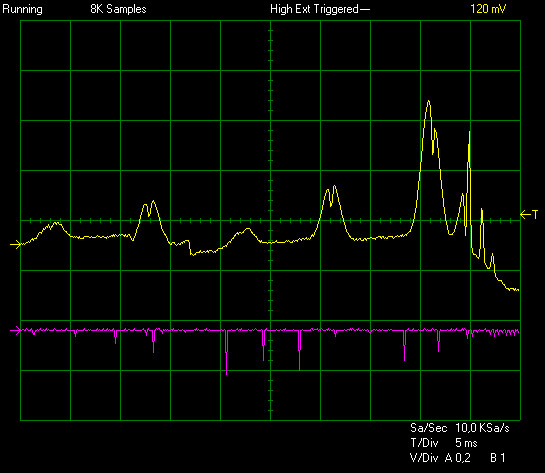
\includegraphics[width=\textwidth]{Figures/2/Tconst20C/117mA.jpg}
        \caption{$I=117$ mA}
        \label{fig:117mA}
    \end{subfigure}
    \begin{subfigure}[b]{0.3\textwidth}
        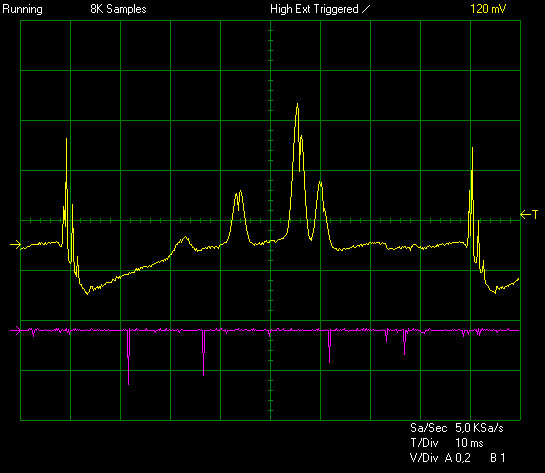
\includegraphics[width=\textwidth]{Figures/2/Tconst20C/118mA.jpg}
        \caption{$I=118$ mA}
        \label{fig:118mA}
    \end{subfigure}
    \begin{subfigure}[b]{0.3\textwidth}
        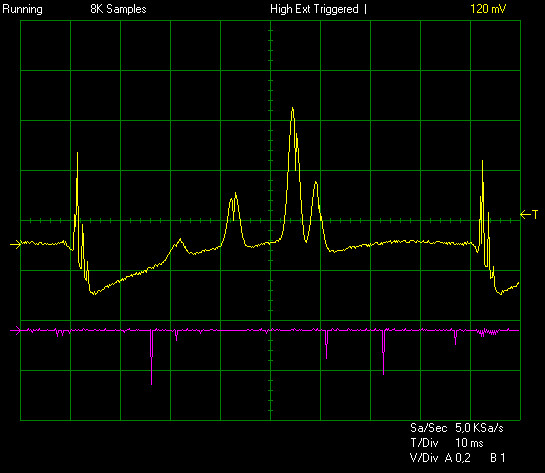
\includegraphics[width=\textwidth]{Figures/2/Tconst20C/119mA.jpg}
        \caption{$I=119$ mA}
        \label{fig:119mA}
    \end{subfigure}
    \begin{subfigure}[b]{0.3\textwidth}
        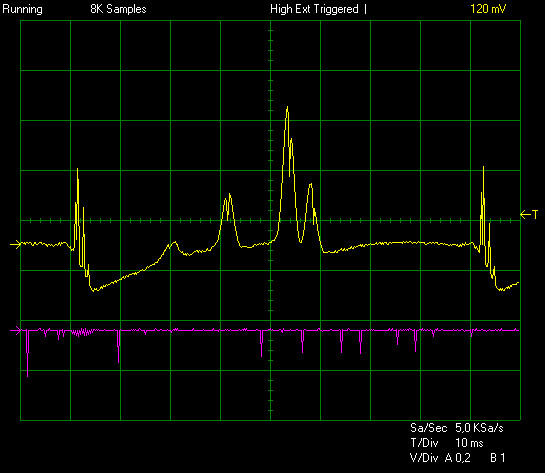
\includegraphics[width=\textwidth]{Figures/2/Tconst20C/120mA.jpg}
        \caption{$I=120$ mA}
        \label{fig:120mA}
    \end{subfigure}
    \begin{subfigure}[b]{0.3\textwidth}
        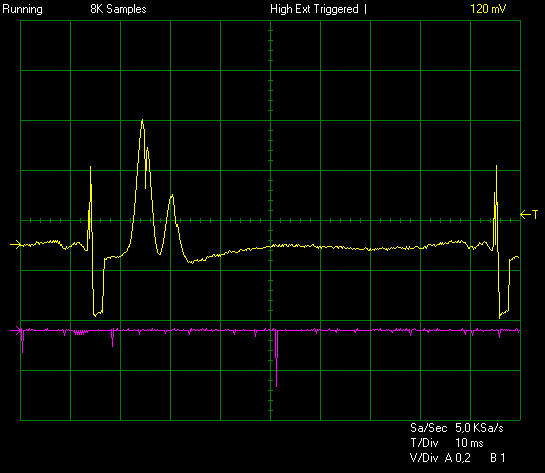
\includegraphics[width=\textwidth]{Figures/2/Tconst20C/121mA.jpg}
        \caption{$I=121$ mA}
        \label{fig:121mA}
    \end{subfigure}
    \begin{subfigure}[b]{0.3\textwidth}
        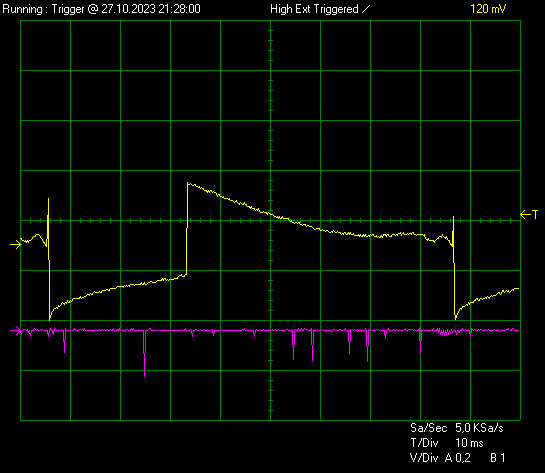
\includegraphics[width=\textwidth]{Figures/2/Tconst20C/122mA.jpg}
        \caption{$I=122$ mA}
        \label{fig:122mA}
    \end{subfigure}
    \caption{Saturation spectra for variation of injection currents}
    \label{fig:VariedCurrent}
\end{figure}

\pagebreak{}

For the case of constant injection current, a mode jump occurs between $T = \SI{19.9}{\celsius}$ and $T = \SI{20.1}{\celsius}$. We notice that changing the current affects the spectrum more drastically. This could be due to the fact that a slight change in the current leads to more heating compared to the temperature increments we used.

\begin{figure}[h]
    \centering
    \begin{subfigure}[b]{0.3\textwidth}
        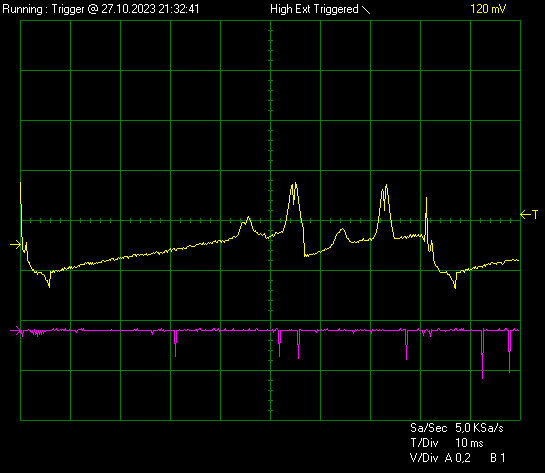
\includegraphics[width=\textwidth]{Figures/2/Iconst118mA/198.jpg}
        \caption{$T = \SI{19.8}{\celsius}$}
        \label{fig:198C}
    \end{subfigure}
    \begin{subfigure}[b]{0.3\textwidth}
        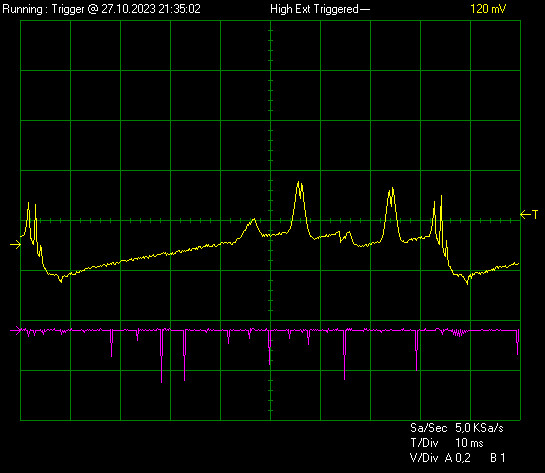
\includegraphics[width=\textwidth]{Figures/2/Iconst118mA/199.jpg}
        \caption{$T = \SI{19.9}{\celsius}$}
        \label{fig:199C}
    \end{subfigure}
    \begin{subfigure}[b]{0.3\textwidth}
        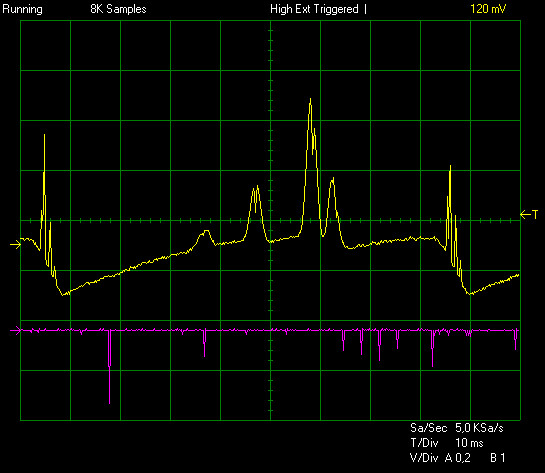
\includegraphics[width=\textwidth]{Figures/2/Iconst118mA/201.jpg}
        \caption{$T = \SI{20.1}{\celsius}$}
        \label{fig:201C}
    \end{subfigure}
    \begin{subfigure}[b]{0.3\textwidth}
        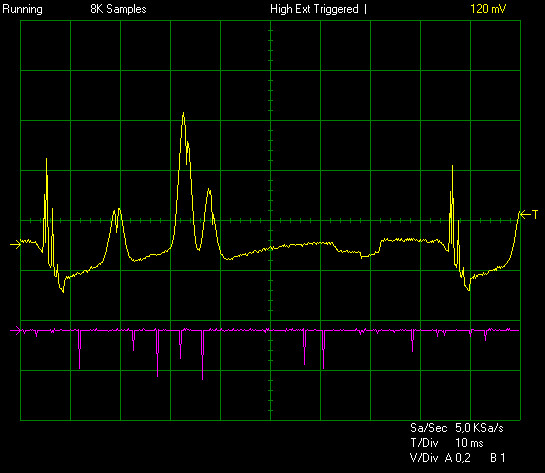
\includegraphics[width=\textwidth]{Figures/2/Iconst118mA/202.jpg}
        \caption{$T = \SI{20.2}{\celsius}$}
        \label{fig:202C}
    \end{subfigure}
    \begin{subfigure}[b]{0.3\textwidth}
        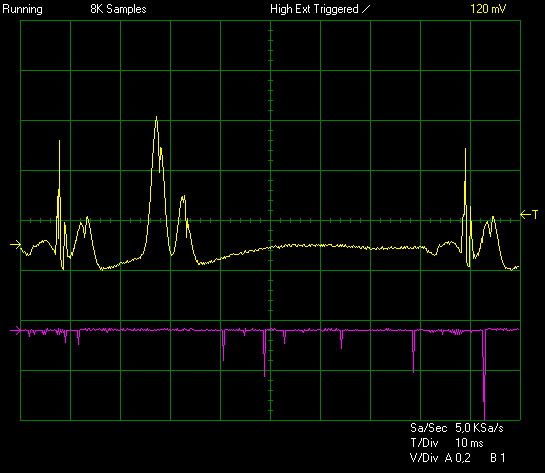
\includegraphics[width=\textwidth]{Figures/2/Iconst118mA/203.jpg}
        \caption{$T = \SI{20.3}{\celsius}$}
        \label{fig:203C}
    \end{subfigure}
    \caption{Saturation spectra for variation of temperature}
    \label{fig:VariedTemperature}
\end{figure}

\pagebreak{}

\subsection{Task 3}

\pagebreak{}

\subsection{Task 4}

\pagebreak{}

\section{Conclusion}

\pagebreak{}

\begin{appendices}


\end{appendices}

\pagebreak{}

\bibliographystyle{ieeetr} 
\bibliography{rbspectroscopy} 

\end{document}